\documentclass{article}


% ready for submission
% \usepackage{neurips_2024}
\usepackage[preprint]{neurips_2024}

\usepackage{graphicx} 
\usepackage[utf8]{inputenc} % allow utf-8 input
\usepackage[T1]{fontenc}    % use 8-bit T1 fonts
\usepackage{hyperref}       % hyperlinks
\usepackage{url}            % simple URL typesetting
\usepackage{booktabs}       % professional-quality tables
\usepackage{amsfonts}       % blackboard math symbols
\usepackage{nicefrac}       % compact symbols for 1/2, etc.
\usepackage{microtype}      % microtypography
\usepackage{xcolor}         % colors
\usepackage{wrapfig}
\usepackage{subcaption}
\usepackage{multirow}
\usepackage{multicol}
\usepackage{array}
\usepackage[usestackEOL]{stackengine}
\usepackage{xspace}
\usepackage{amsmath}
\usepackage[most]{tcolorbox}
 
\newcommand{\hide}[1]{}

\newcommand{\model}{CogVideoX\xspace} 
\newcommand{\dong}[1]{\textbf{\color{red}[(Dong: #1 )]}}
\newcommand{\gxt}[1]{\textbf{\color{cyan}[Gu: #1 ]}}

\newcommand{\fix}{\marginpar{FIX}}
\newcommand{\new}{\marginpar{NEW}}

\newcommand{\aspace}{\hspace{1em}}

\newtcolorbox{promptbox}[1][]{
  breakable,
  title=#1,
  colback=gray!5,
  colframe=black,
  colbacktitle=gray!15,
  coltitle=black,
  fonttitle=\bfseries,
  bottomrule=1.5pt,
  toprule=1.5pt,
  leftrule=1pt,
  rightrule=1pt,
  arc=0pt,
  outer arc=0pt,
  enhanced,
  before upper={\parindent=1.5em}
}


% author formatting
\usepackage{authblk}
\renewcommand\Authands{, } %
\renewcommand{\Authfont}{\bfseries}
\makeatletter
\renewcommand\AB@affilsepx{, \protect\Affilfont}
\makeatother

\title{

\includegraphics[width=0.07\textwidth]{images/logo.png}
CogVideoX: Text-to-Video Diffusion Models with An Expert Transformer}

\author{Zhuoyi Yang$^{\star}$ \aspace  Jiayan Teng$^{\star}$ \aspace  Wendi Zheng  \aspace Ming Ding \aspace  Shiyu Huang \aspace Jiazheng Xu \\
Yuanming Yang\aspace  Wenyi Hong\aspace  Xiaohan Zhang \aspace Guanyu Feng \aspace Da Yin  \\
\aspace Xiaotao Gu  \aspace  Yuxuan Zhang \aspace Weihan Wang  \aspace Yean Cheng  \aspace Ting Liu \aspace   Bin Xu   \aspace \\
  Yuxiao Dong \aspace  Jie Tang \\ 
~\\ 
\textnormal{Zhipu AI \aspace Tsinghua University}
}
% \affil[]{Zhipu AI \aspace Tsinghua University}
\affil[]{}


%  \hide{
% \author{Zhuoyi Yang$^{\star}$ \aspace {\bf Jiayan Teng}$^{\star}$ \aspace {\bf Wendi Zheng} \aspace {\bf Ming Ding} \aspace {\bf Shiyu Huang} \\
% \aspace {\bf Jiazheng Xu} \aspace
% {\bf Yuanming Yang} \aspace {\bf Xiaohan Zhang} \aspace {\bf Xiaotao Gu} \aspace  {\bf Guanyu Feng}\aspace \\
%  {\bf Da Yin} 
% \aspace {\bf Wenyi Hong} \aspace  {\bf Weihan Wang} \aspace
%  {\bf Yean Cheng} \aspace {\bf Yuxuan Zhang} \aspace  \\
%  {\bf Ting Liu} \aspace {\bf Bin Xu}  \aspace {\bf Yuxiao Dong} \aspace {\bf Jie Tang}~\\
% $^{1}$Zhipu AI \aspace $^{2}$Tsinghua University\\
% \textmd{\href{https://github.com/THUDM/CogVideo}{https://github.com/THUDM/CogVideo}} 
% }
% }

% $^1$Zhipu AI\ \ \ \ \ \ $^2$Tsinghua University 
% \href{https://github.com/THUDM/CogVideo}{https://github.com/THUDM/CogVideo}
 



% \renewcommand{\thefootnote}{}
% \footnotetext{Zhuoyi and Jiayan made equal contributions. Core contributors: Zhuoyi, Jiayan, Wendi, Ming, and Shiyu.}
% \footnotetext{{\{yangzy22,tengjy20\}@mails.tsinghua.edu.cn, \{yuxiaod,jietang\}@tsinghua.edu.cn}}
% %\footnotetext{$^\dagger$ corresponding authors}
% \renewcommand{\thefootnote}{\arabic{footnote}}

\begin{document}


\maketitle

\renewcommand{\thefootnote}{}
\footnotetext{*Equal contributions. Core contributors: Zhuoyi, Jiayan, Wendi, Ming, and Shiyu.}
\footnotetext{{\{yangzy22,tengjy24\}@mails.tsinghua.edu.cn, \{yuxiaod,jietang\}@tsinghua.edu.cn}}
\renewcommand{\thefootnote}{\arabic{footnote}}


\begin{abstract}
We introduce \model, large-scale diffusion transformer models designed for generating videos based on text prompts. 
To efficently model video data, we propose to levearge a 3D Variational Autoencoder (VAE) to compress videos along both spatial and temporal dimensions. 
To improve the text-video alignment, we propose an expert transformer with the expert adaptive LayerNorm to facilitate the deep fusion between the two modalities. 
By employing a progressive training technique, \model is adept at producing coherent, long-duration videos characterized by significant motions. 
In addition, we develop an effective text-video data processing pipeline that includes various data preprocessing strategies and a video captioning method. 
It significantly helps enhance the performance of \model, improving both generation quality and semantic alignment. 
Results show that \model demonstrates state-of-the-art performance across both multiple machine metrics and human evaluations. 
The model weights of both the 3D Causal VAE and \model are publicly available at \url{https://github.com/THUDM/CogVideo}. 
% and \url{https://huggingfaces.co/THUDM/CogVideoX}. 

%We introduce CogVideoX, a large-scale diffusion transformer model designed for generating videos based on text prompts. The model leverages a 3D Variational Autoencoder (VAE) and a 3D expert transformer, utilizing Expert Adaptive LayerNorm. By employing a progressive training technique, CogVideoX is adept at producing coherent, long-duration videos characterized by significant motion. Additionally, we introduce a comprehensive large-scale data processing pipeline that includes various data cleaning strategies and a novel video captioning method, resulting in enhanced generation quality and improved semantic alignment. CogVideoX demonstrates state-of-the-art performance across multiple machine metrics and human evaluations.
\end{abstract}

\section{Introduction}

In recent years, diffusion models have made groundbreaking advancements in multimodal generation, such as image, video, speech and 3D generation. Among these, video generation is a rapidly evolving field and being extensively explored. Given the successful experiences with Large Language Models (LLMs), comprehensive scaling up of data volume, training iterations, and model size consistently enhances model performance. Additionally, there is more mature scaling experience with transformers compared to UNet. And DiT \citep{peebles2023scalable} has shown that transformers can effectively replace UNet as the backbone of diffusion models. Thus, transformer is a better choice for video generation.
However, long-term consistent video generation remains a significant challenge.  % 第一段介绍任务重要性和我们工作的亮点,例如开源。DiT的讨论不应该在这里

The first challenge is that constructing a web-scale video data pipeline is considerably more difficult than for textual data. Video data is extremely diverse in distribution, quality varies greatly, and simple rule-based filtering is often insufficient for effective data selection. Consequently, processing video data is both time-consuming and highly complex.
There are numerous meaningless unrealistic videos, such as poor-quality edits and computer screen recordings. And many videos are difficult to watch normally, such as those with excessively shaky cameras. These types of data are harmful to the generative model's ability to learn genuine dynamic information. They need to be meticulously processed and filtered out to ensure the quality of the training dataset.

Additionally, most video data available online lacks accurate textual descriptions, significantly limiting the model's ability to grasp precise semantic understanding. To address this issue, we trained a video understanding model capable of accurately describing video content. We use it to generate new textual descriptions for all video data. 
To advance the field of video generation, we have decided to open-source this description model.

The high training cost is another significant challenge. If the video is unfolded into a one-dimensional sequence in the pixel space, the length would be extraordinarily long. To keep the computational cost within a feasible range, we trained a 3D VAE that compresses the video along both spatial and temporal dimensions. Additionally,  unlike previous video models that use a 2D VAE to encode each frame separately, 3D VAE ensures continuity among frames so that the generated videos do not flicker. 

Moreover, to improve the alignment between videos and texts, we propose an expert transformer to facilitate the interaction between the two modalities. Then, to ensure the consistency of video generation and to capture large-scale motions, it is necessary to comprehensively model the video along both temporal and spatial dimensions. Therefore, we opt for 3D full attention, as detailed in Section~\ref{sec:expert-transformer}.



\section{The \model Architecture}\label{sec:model}


In the section, we present the \model model. 
Figure \ref{fig:model} illustrates the overall architecture. 
Given a pair of video and text input,  we design a \textbf{3D causal VAE} to compress the video into the latent space, and the latents are then patchified and unfolded into a long sequence denoted as $z_{\text{vision}}$. 
Simultaneously, we encode the textual input into text embeddings $z_{\text{text}}$ using T5~\citep{raffel2020exploring}. 
Subsequently, $z_{\text{text}}$ and $z_{\text{vision}}$ are concatenated along the sequence dimension. 
The concatenated embeddings are then fed into a stack of \textbf{expert transformer} blocks.
Finally, the model output are unpatchified to restore the original latent shape, which is then decoded using a 3D causal VAE decoder to reconstruct the video. 
We illustrate the technical design of the 3D causal VAE and expert transfomer in detail.


\begin{figure}[h]
\begin{center}
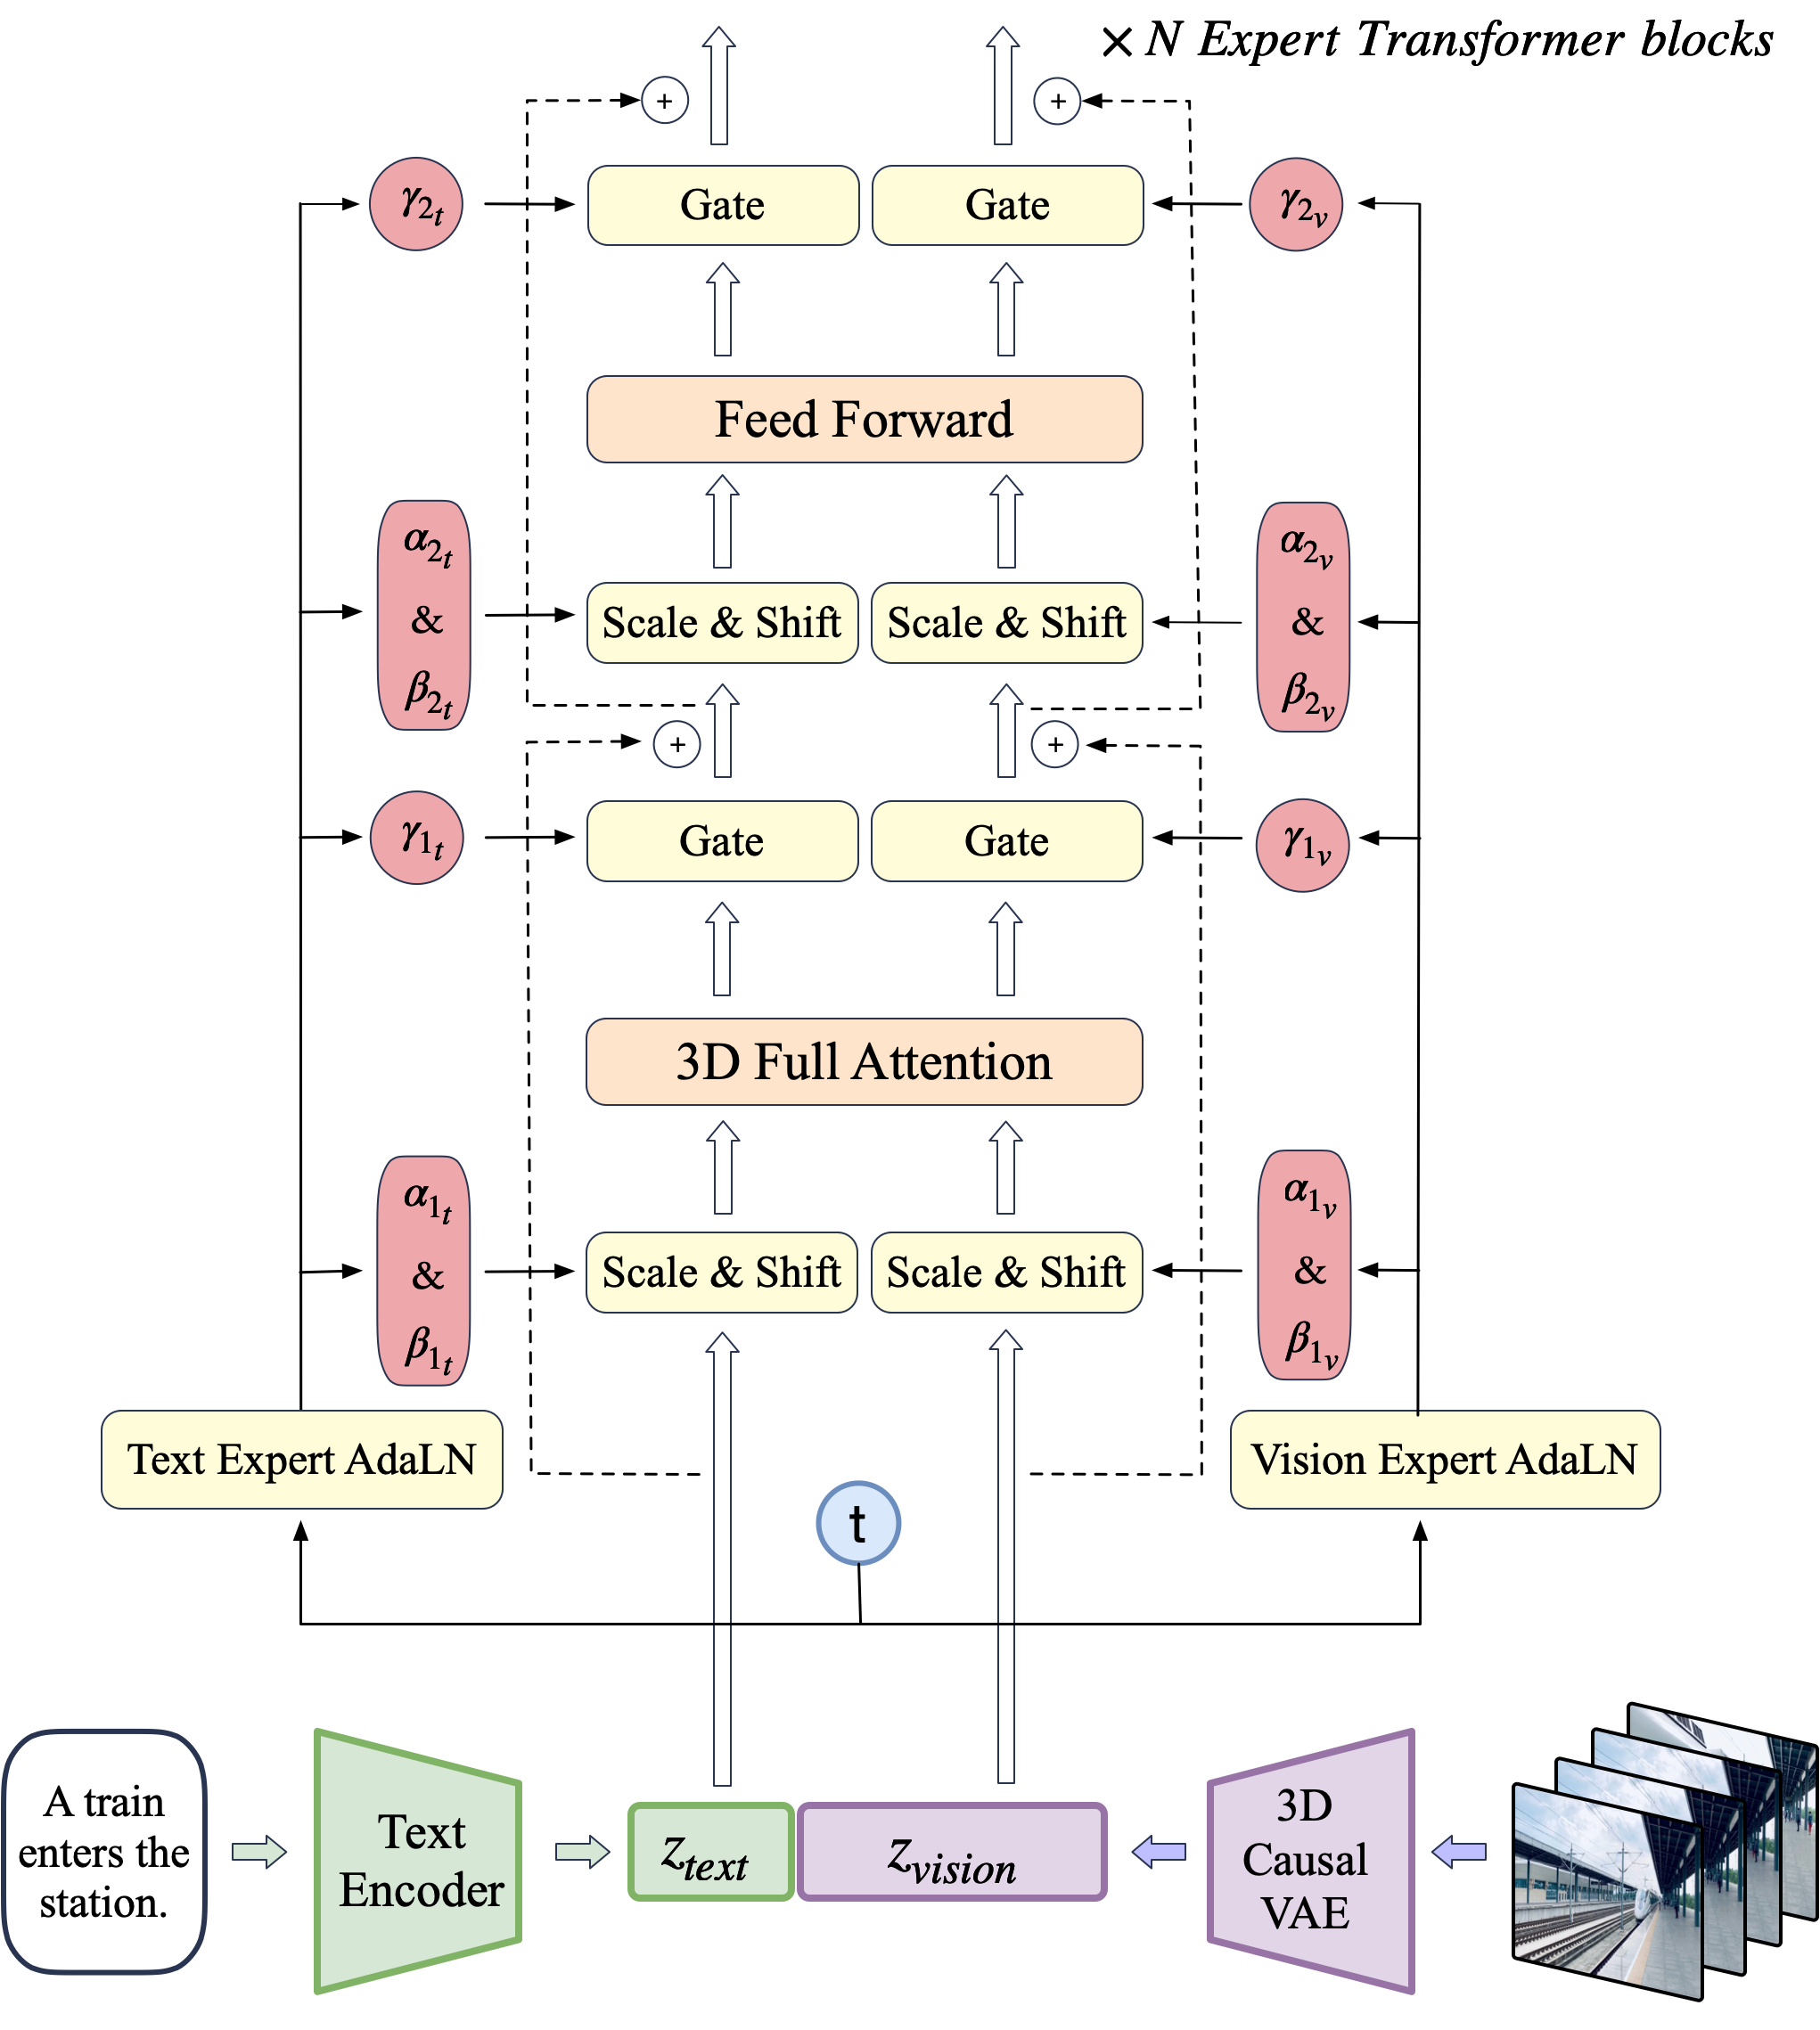
\includegraphics[width=0.7\linewidth]{images/transformer.png}
\end{center}
\caption{\textbf{The overall architecture of \model.} }
\label{fig:model}
\end{figure}



\subsection{3D Causal VAE} 

%Compared to image data, 

Videos encompass not only spatial information but also substantial temporal information, usually resulting in orders of magnitude more data volumes than images.  
To tackle the computational challenge of modeling video data, we propose to implement a video compression module based on 3D Variational Autoencoders (3D VAEs)~\citep{yu2023language}.
%Our 3D VAE
The idea is to incorporate three-dimentional convolutions to compress videos both spatially and temporally. 
This can help achieve a higher compression ratio with largely improved quality and continuity of video reconstruction when compared to previous image VAEs~\citep{rombach2022high, esser2021taming}. 
\begin{figure}[h]
\begin{center}
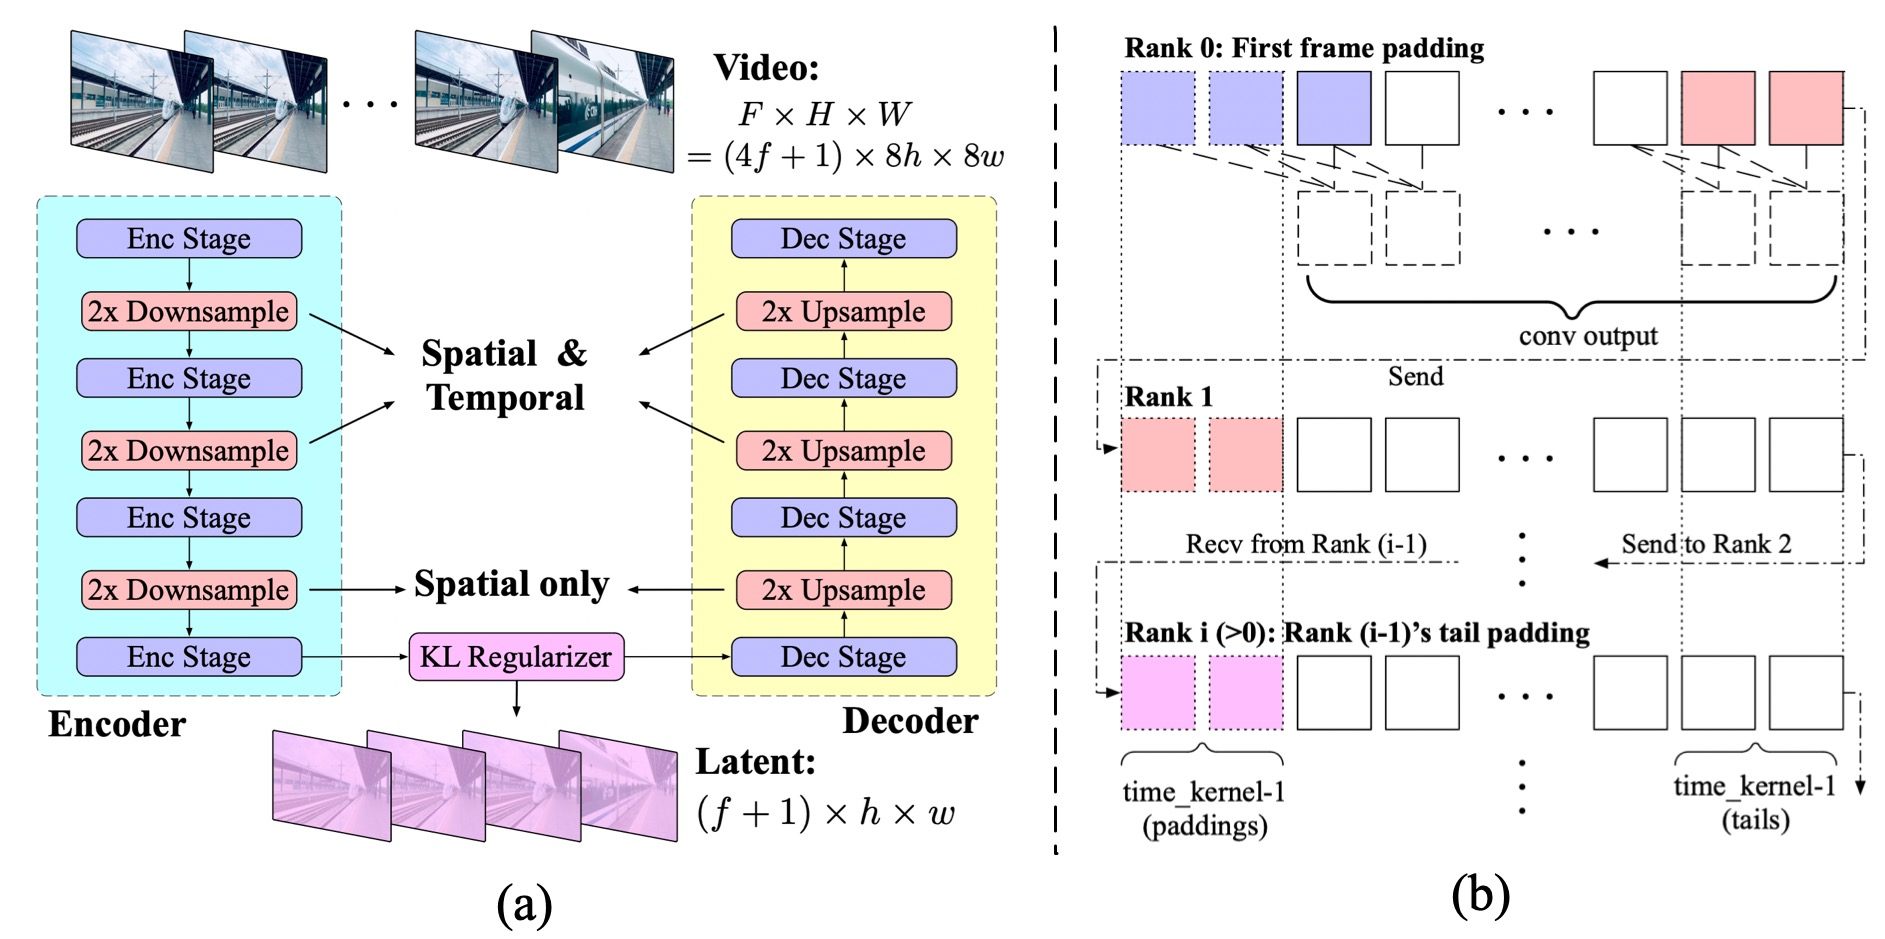
\includegraphics[width=\linewidth]{images/3dvae_combined.jpg}
\end{center}
\caption{(a) The structure of the 3D VAE in \model. It comprises an encoder, a decoder and a latent space regularizer, achieving a 4$\times$8$\times$8 compression from pixels to the latents. (b) The context parallel implementation on the temporally causal convolution.}
\label{fig:3dvae_combined}
\end{figure}

Figure~\ref{fig:3dvae_combined} (a) shows the structure of the proposed 3D VAE. 
It comprises an encoder, a decoder and a latent space regularizer. 
The Gaussian latent space is constrained by a Kullback-Leibler (KL) regularizer.
The encoder and decoder consist of four symmetrically arranged stages, respectively performing 2$\times$ downsampling and upsampling by the interleaving of ResNet block stacked stages. 
The first two rounds of downsampling and the last two upsampling involve both the spatial and temporal dimensions, while the last round only applies spatial sampling. 
This enables the 3D VAE to achieve a 4$\times$ compression in the temporal dimension and an 8$\times$8 compression in the spatial dimension. 
In total, this achieves a 4$\times$8$\times$8 compression from pixels to the latents. 

We adopt the temporally causal convolution~\citep{yu2023language}, which places all the paddings at the beginning of the convolution space, as shown in Figure~\ref{fig:3dvae_combined} (b). 
This ensures the future information not to influence the present or past predictions. 
Given that processing videos with a large number of frames introduces excessive GPU memory usage, we apply context parallel at the temporal dimension for 3D convolution to distribute computation among multiple devices. 
As illustrated by Figure~\ref{fig:3dvae_combined} (b), due to the causal nature of the convolution, each rank simply sends a segment of length $k-1$ to the next rank, where $k$ indicates the temporal kernel size. 
This results in relatively low communication overhead.

During actual implementation, we first train a 3D VAE on lower resolutions and fewer frames to save computation. 
We observe that the encoding of larger resolution generalizes naturally, while extending the number of frames to be encoded does not work as seamlessly. 
Therefore, we conduct a two-stage training process by first training on short videos and finetuning by context parallel on long videos. 
Both stages of training utilize a weighted combination of the L2 loss, LPIPS~\citep{zhang2018unreasonable} perceptual loss, and GAN loss from a 3D discriminator.

\begin{figure}[h]
\begin{center}
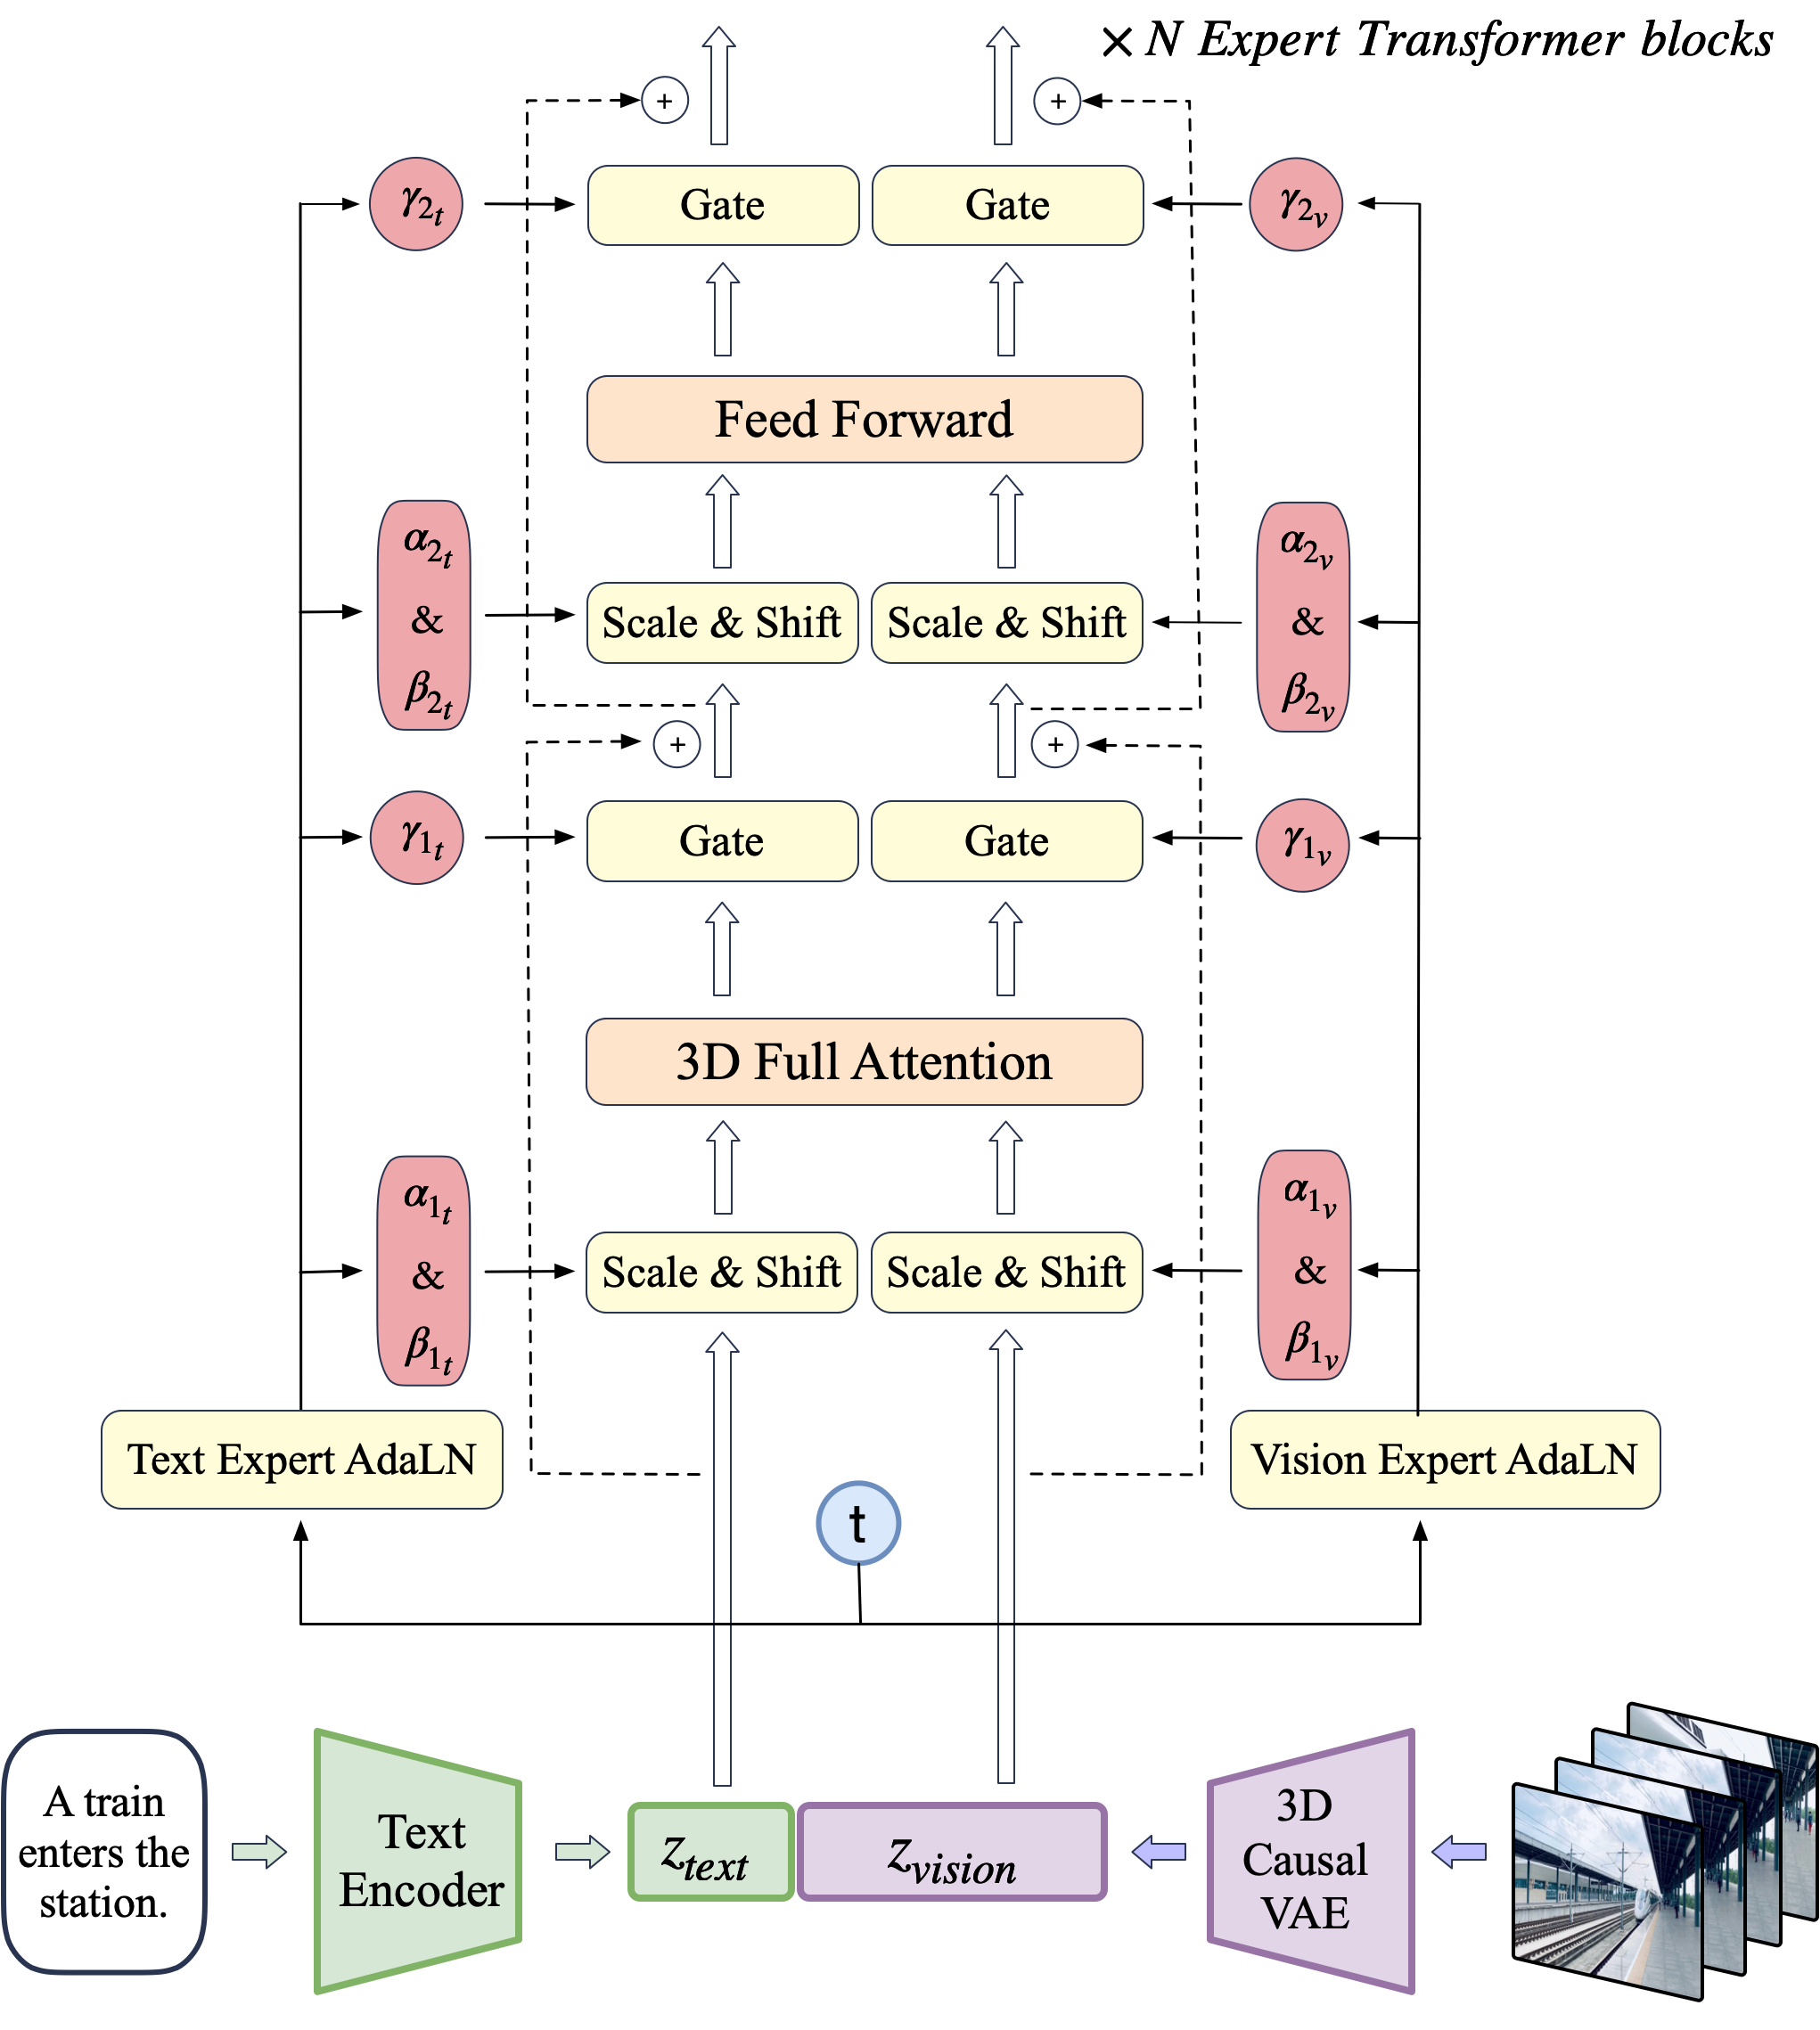
\includegraphics[width=0.7\linewidth]{images/transformer.png}
\end{center}
\caption{\textbf{Our model architecture.} }
\label{fig:model}
\end{figure}

\subsection{Expert Transformer}\label{sec:expert-transformer}

\paragraph{Patchify}
After being encoded into latent vectors of shape $T \times H \times W \times C$ by the 3D causal VAE, the video latents are patchified  along the spatial dimensions, resulting sequence $z_{\text{vision}}$ of length $T\cdot \frac{H}{p} \cdot \frac{W}{p}$. 
% VAE encodes the video into a latent vector of shape $T \times H \times W \times C$. Then we patchify the latent along the spatial dimensions, generating sequence $z_{vision}$ of length $T\cdot \frac{H}{p} \cdot \frac{W}{p}$. 
We do not patchify along the temporal dimension in order to enable joint training of images and videos.

\paragraph{3D-RoPE}
Rotary Position Embedding (RoPE)~\citep{su2024roformer} is a relative positional encoding that has been demonstrated to capture inter-token relationships effectively in LLMs, particularly excelling in modeling long sequences. To adapt to video data, we extend RoPE to 3D. 
Each latent in the video tensor can be represented by a 3D coordinate $(x, y, t)$.
We independently apply 1D-RoPE to each dimension of the coordinates, each occupies $3/8$, $3/8$, $2/8$ of the hidden states's channel. The resultsing encoding are then concatenate along the channel dimension to obtain the final 3D-RoPE encoding.

\paragraph{Expert Transformer Block}
We concatenate the embeddings of both text and video at the input stage to better align visual and semantic information. However, the feature spaces of these two modalities differ significantly, and their embeddings may even have different numerical scales. To better process them within the same sequence, we employ Expert Adaptive Layernorm to handle each modality independently.
As shown in Figure~\ref{fig:model}, following DiT~\citep{peebles2023scalable}, we use the timestep $t$ of the diffusion process as the input to the modulation module. 
Then, the Vision Expert Adaptive Layernorm and Text Expert Adaptive Layernorm independently apply this modulation mechanism to the vision hidden states and text hidden states respectively. This method promotes the alignment of feature spaces across two modalities while minimizing additional parameters.



\paragraph{3D Full Attention}
Previous works \citep{singer2022make, guo2023animatediff} often employ separated spatial and temporal attention to reduce computational complexity and facilitate fine-tuning from text-to-image models. However, as illustrated in Figure~\ref{fig:attention}, this separated attention approach requires extensive implicit transmission of visual information, significantly increasing the learning complexity and making it challenging to maintain the consistency of large-movement objects. Considering the great success of long-context training in LLMs and the efficiency of FlashAttention, we propose a 3D text-video hybrid attention mechanism. This mechanism not only achieves better results but can also be easily adapted to various parallel acceleration methods. 


\begin{wrapfigure}{r}{0.5\textwidth}
\centering
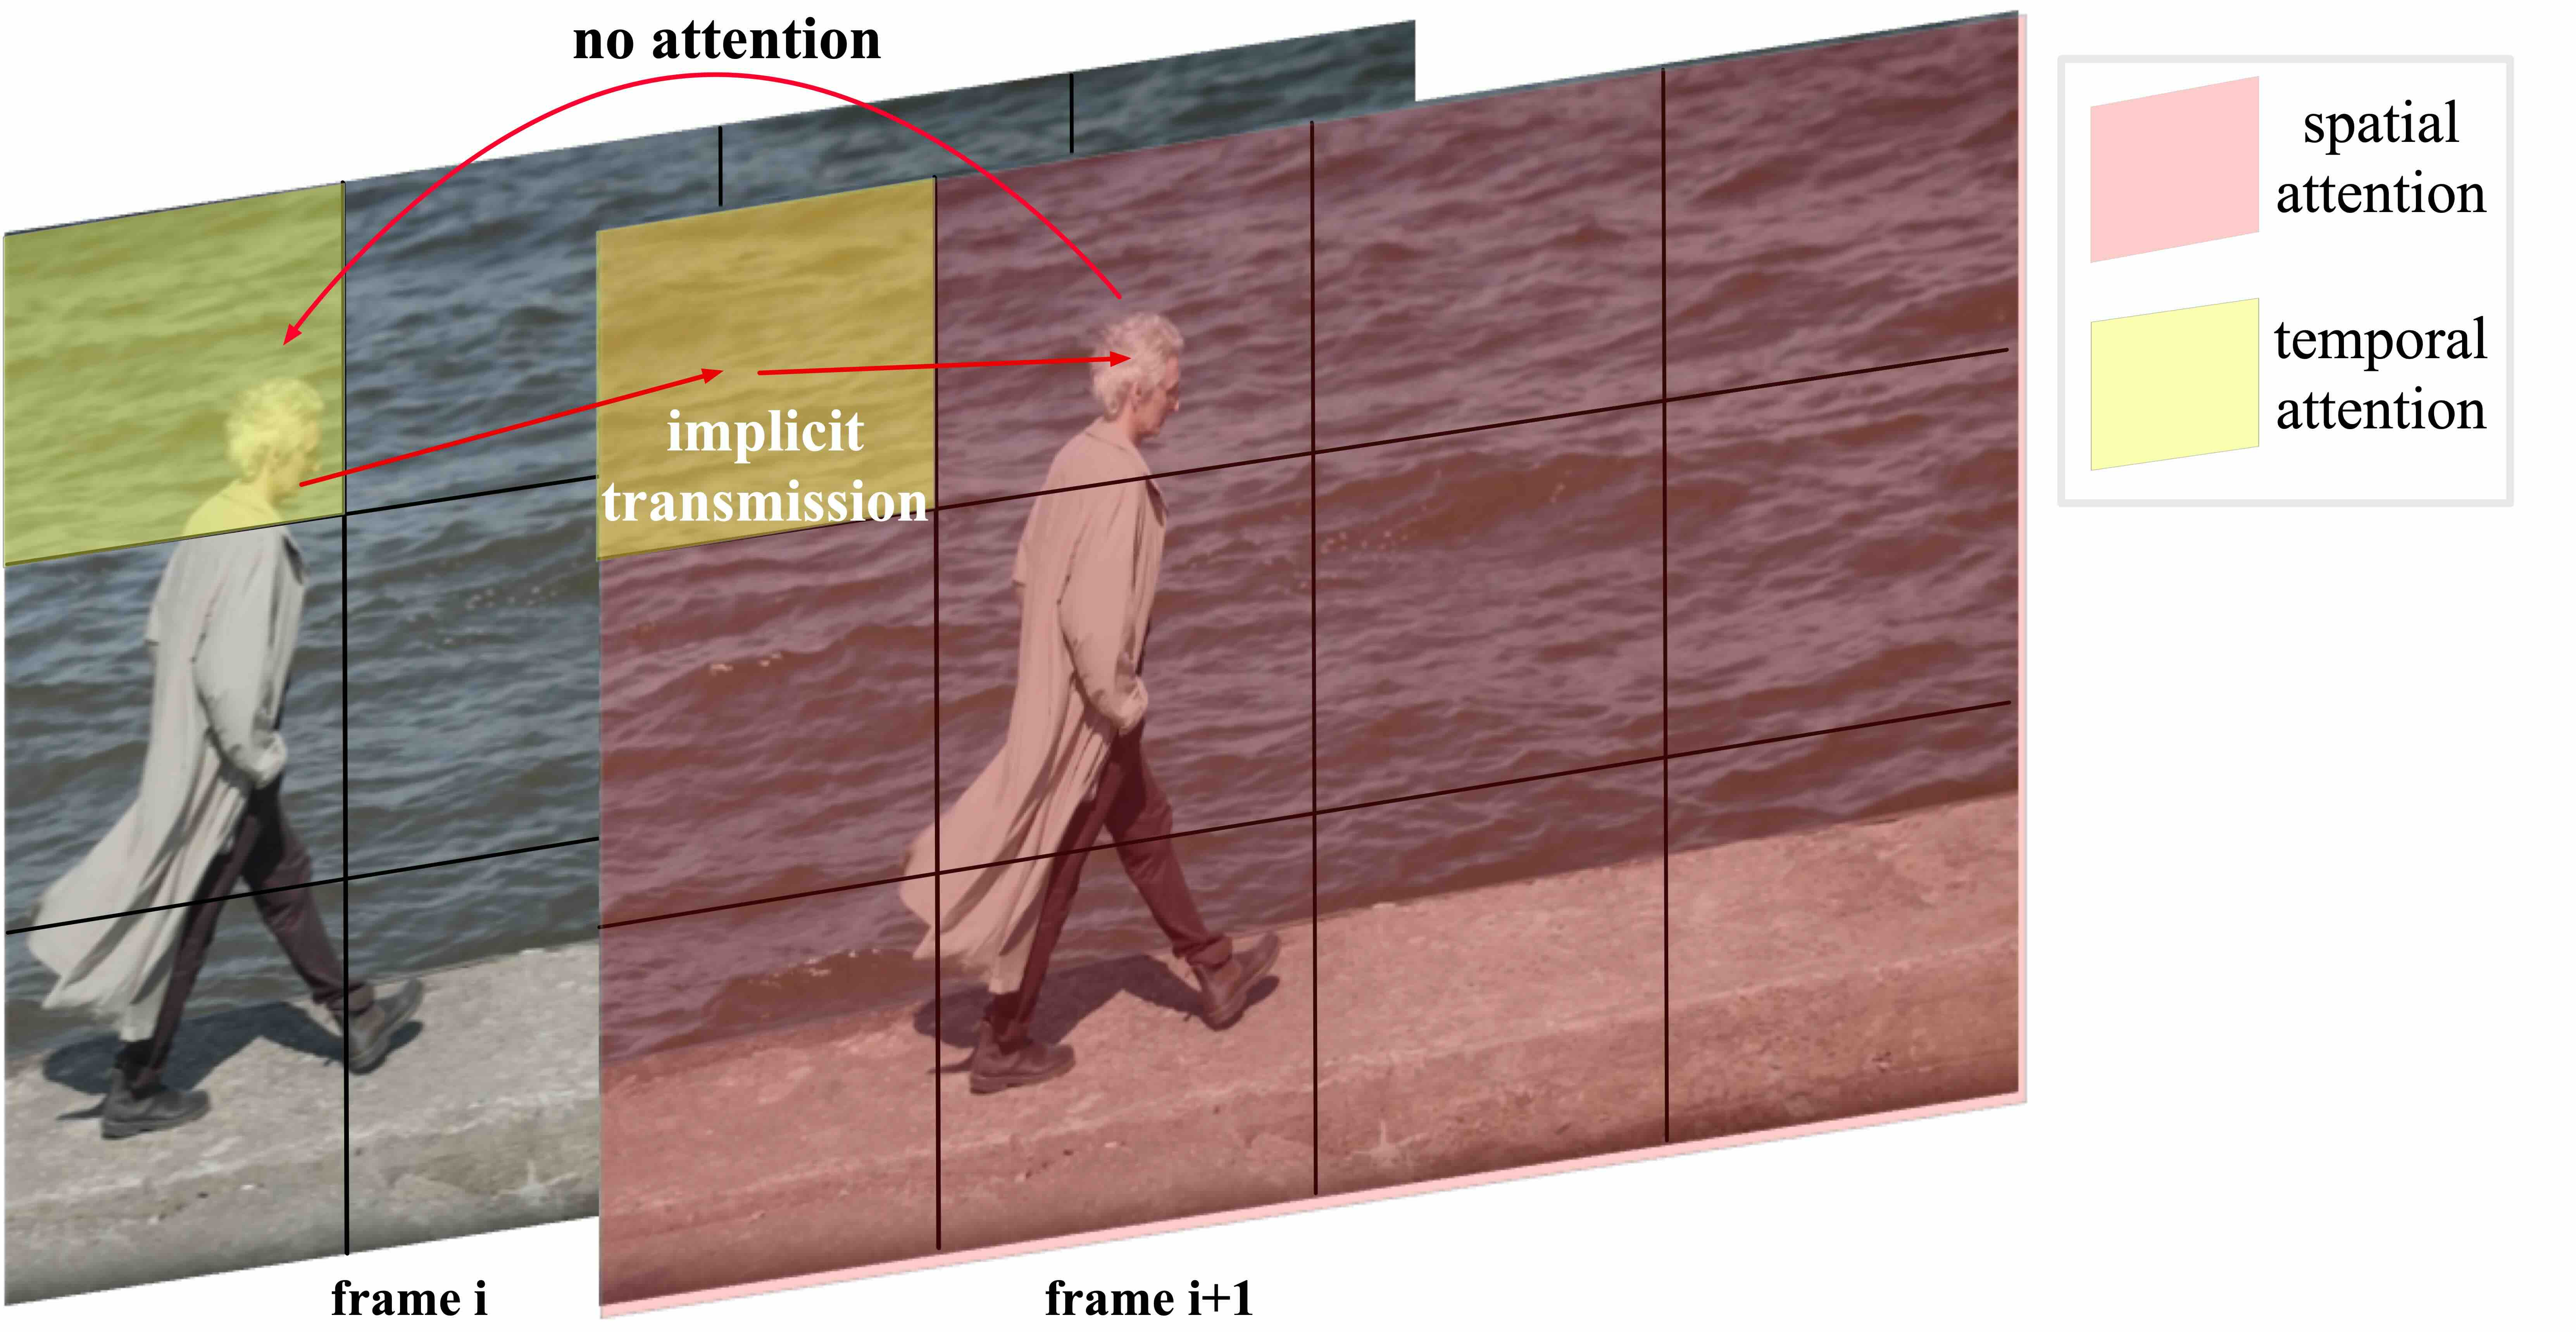
\includegraphics[width=\linewidth]{images/attention.png}
\caption{The separated spatial and temporal attention makes it challenging to  handle the large motion between adjacent frames. In the figure, the head of the person in frame $i+1$ cannot directly attend to the head in the frame $i$. Instead, visual information can only be implicitly transmitted through other background patches. This can lead to inconsistency issues in the generated videos.}
\label{fig:attention}
\vspace{-10mm}
\end{wrapfigure}




\begin{figure}[ht]
\begin{center}
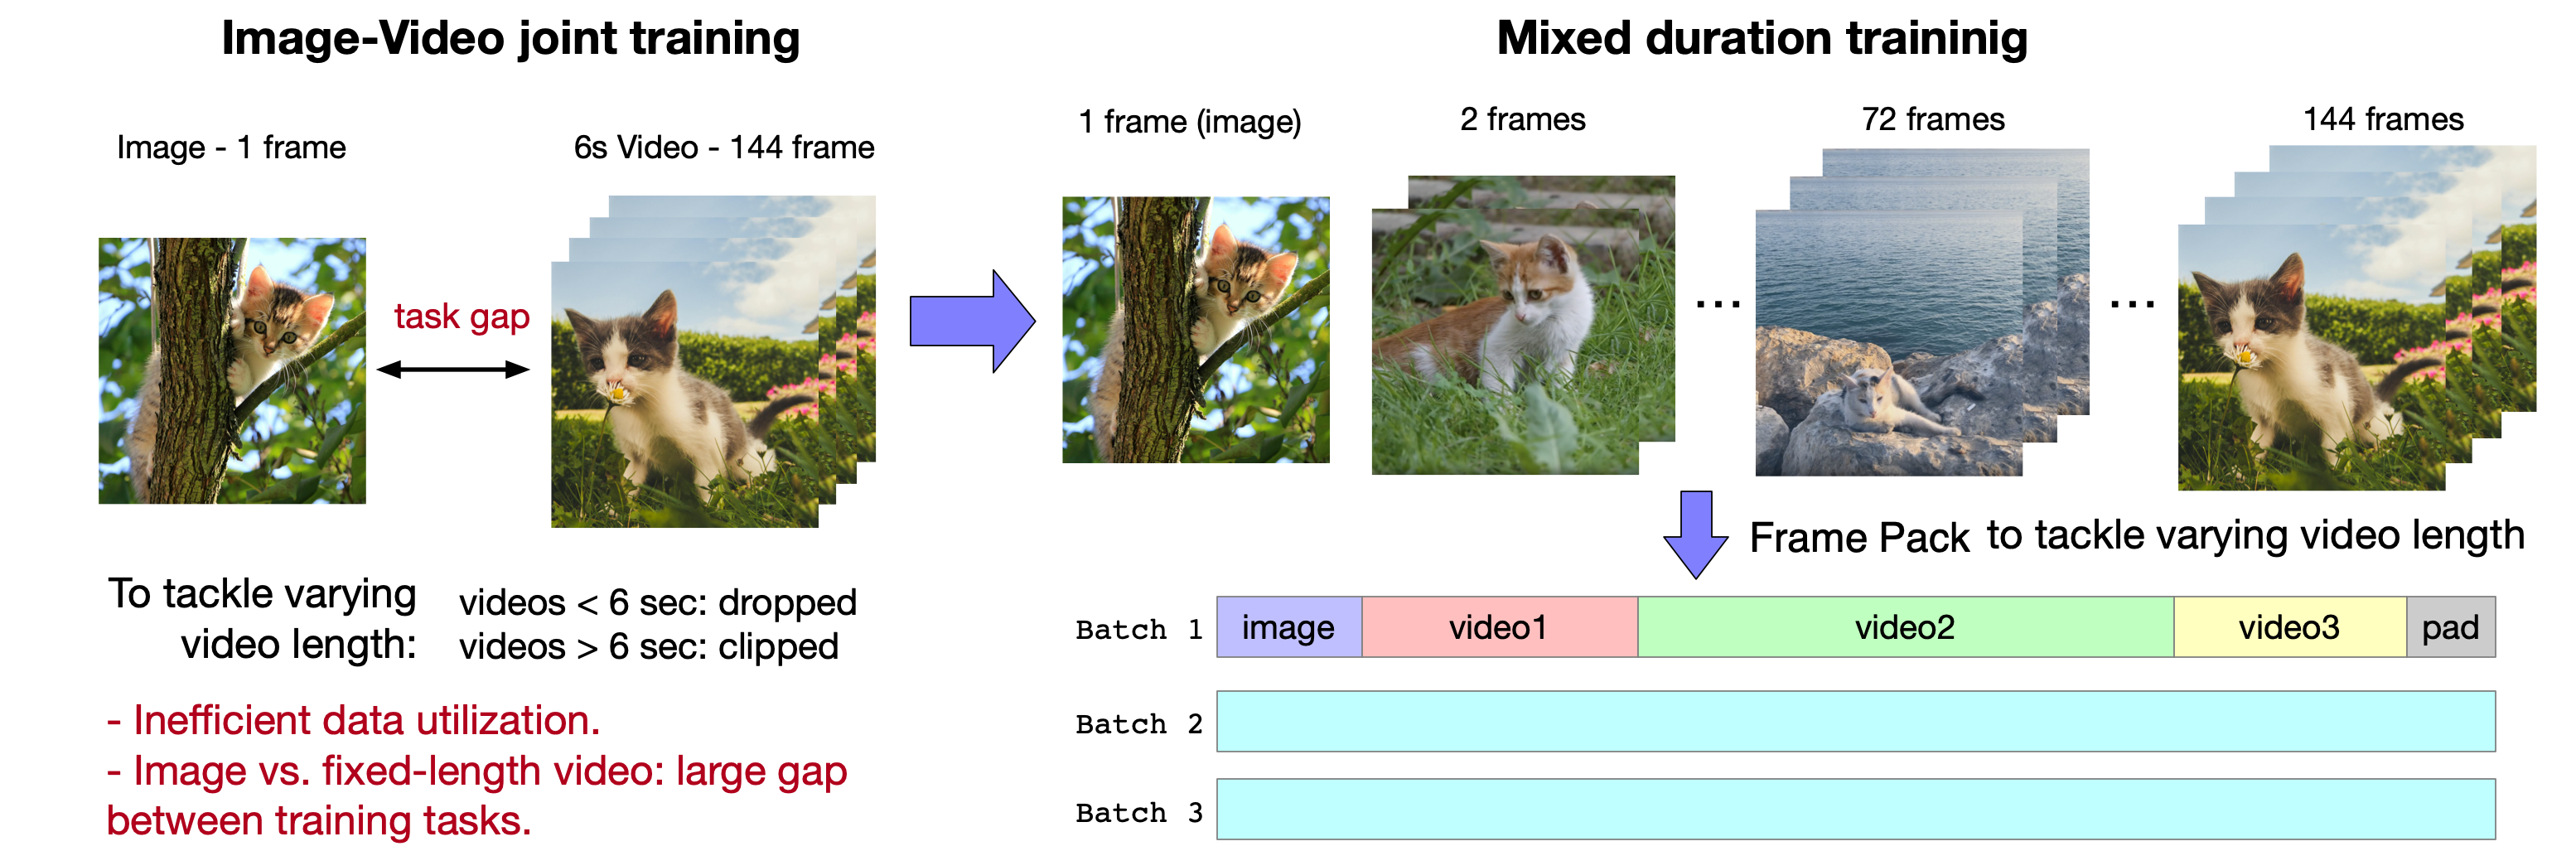
\includegraphics[width=\linewidth]{images/CogVideoX.png}
\end{center}
\caption{
The diagram of mixed-duration training and Frame Pack. To fully utilize the data and enhance the model's generalization capability, we train with videos of different durations within the same batch.}
\label{fig:framepack}
\end{figure}

\section{Training \model}

%\subsection{Setting}
We mix images and videos during training, treating each image as a single-frame video. 
Additionally, we employ progressive training from the resolution perspective. 
For the diffusion setting, we adopt v-prediction~\citep{salimans2022progressive} and zero SNR~\citep{lin2024common}, following the noise schedule used in LDM~\citep{rombach2022high}.
During diffusion training for timestep sampling, we also employ an explicit uniform timestep sampling method, which benefits training stability. 

\subsection{Frame Pack}
Previous video training methods often involve joint training of images and videos with fixed number of frames~\citep{singer2022make, blattmann2023stable}. 
However, this approach usually leads to two issues: 
First, there is a significant gap between the two input types using bidirectional attention, with images having one frame while videos having dozens of frames. 
We observe that models trained this way tend to diverge into two generative modes based on the token count and not to have good generalizations. %e well. 
Second, to train with a fixed duration, we have to discard short videos and truncate long videos, which prevents full utilization of the videos of varying number of frames.

To address these issues, we choose mixed-duration training, which means training videos of different lengths together. 
However, inconsistent data shapes within the batch make training difficult. 
Inspired by Patch'n Pack \citep{dehghani2024patch}, we place videos of different lengths into the same batch to ensure consistent shapes within each batch, a method we refer to as \textit{Frame Pack}. The process is illustrated in Figure~\ref{fig:framepack}. 

\subsection{Resolution Progressive Training}

The training pipeline of \model is divided into three stages: low-resolution training, high-resolution training, and high-quality video fine-tuning. 
Similar to images, videos from the Internet usually include a significant amount of low-resolution ones. 
Progressive training can effectively utilize videos of various resolutions. 
Moreover, training at low resolution initially can equip the model with coarse-grained modeling capabilities, followed by high-resolution training to enhance its ability to capture fine details. 
Compared to direct high-resolution training, staged training can also help reduce the overall training time.

\begin{figure}[h]
\begin{center}
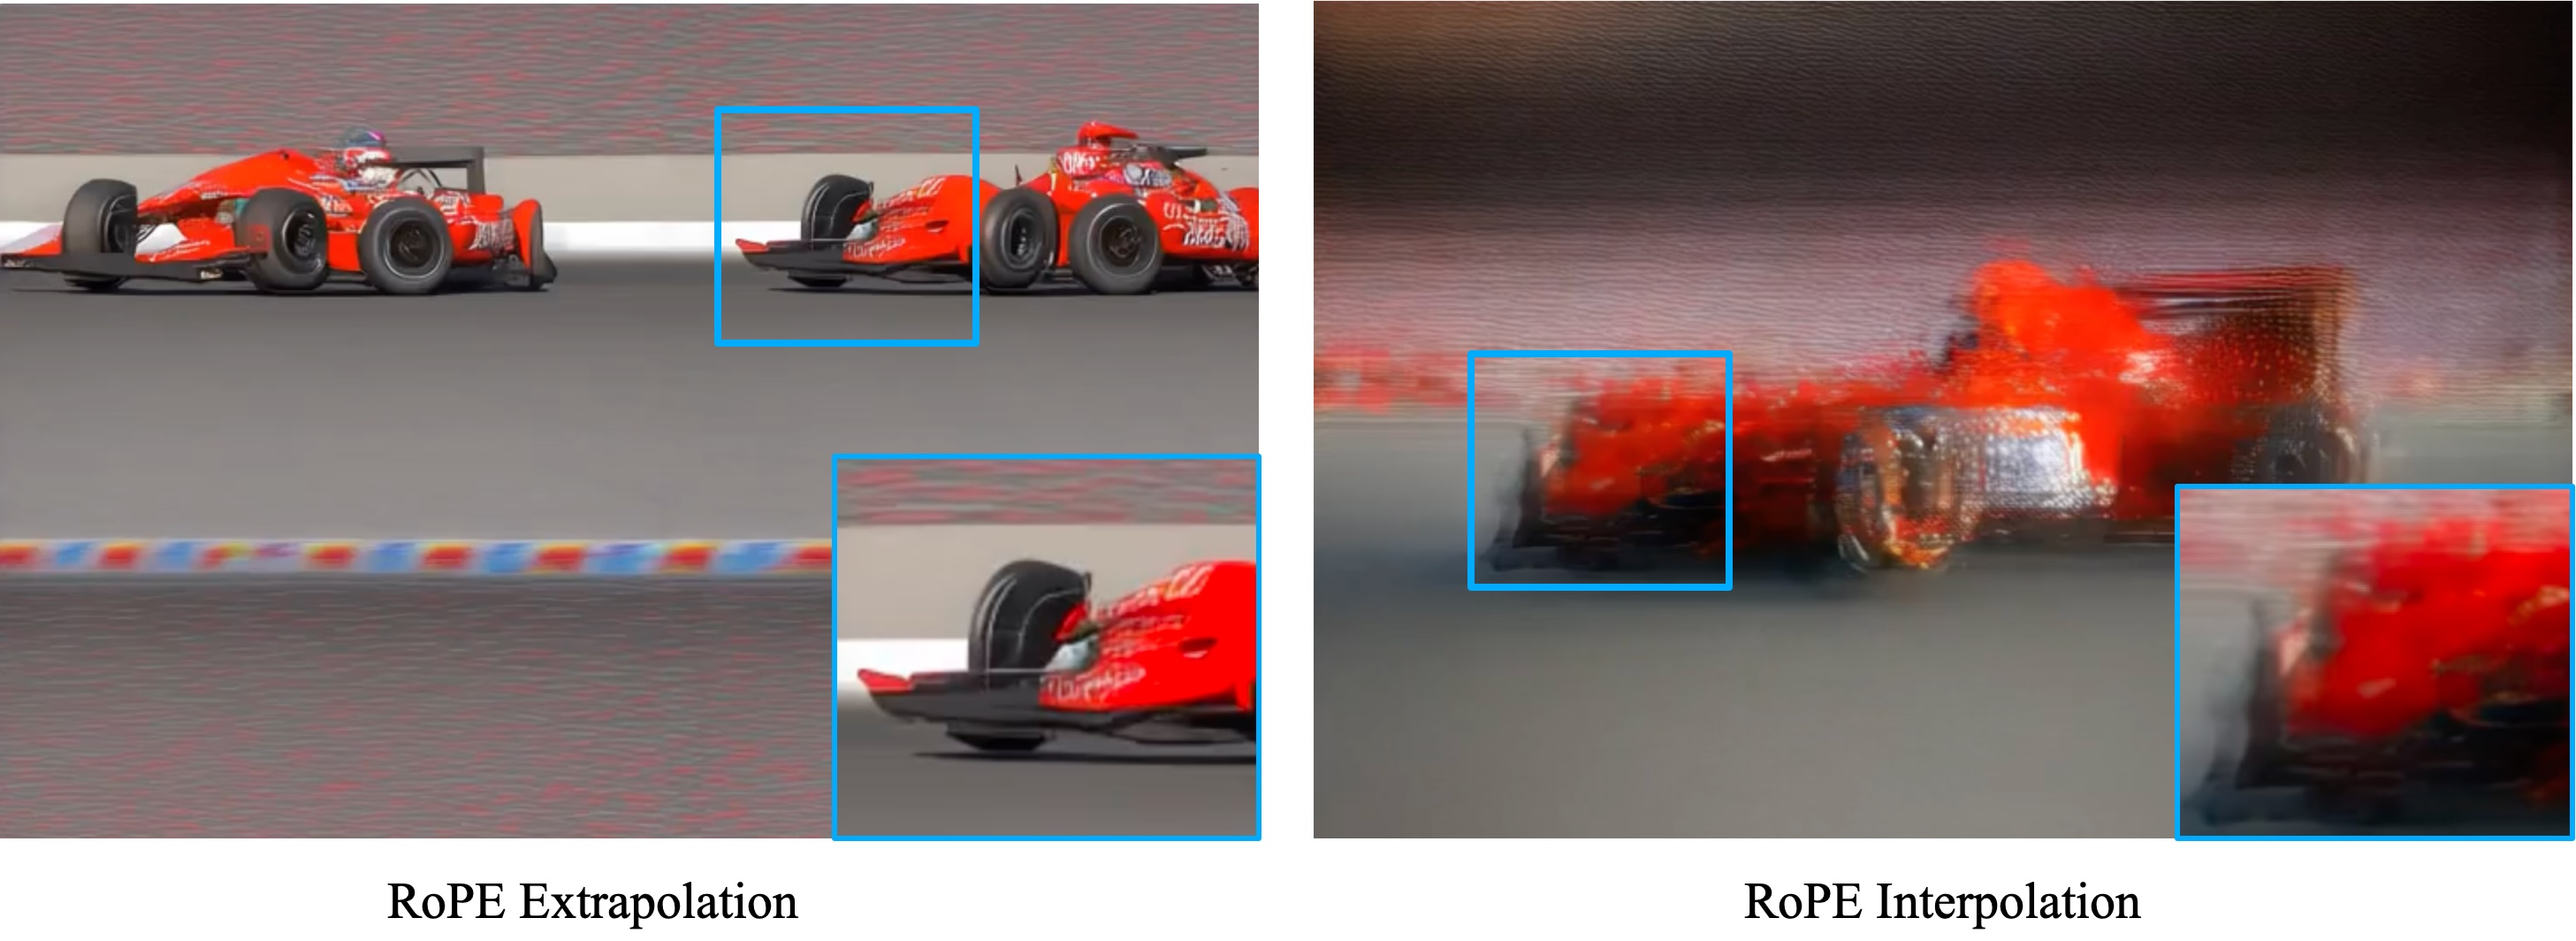
\includegraphics[width=0.9\linewidth]{images/ive.jpg}
\end{center}
\caption{The comparison between the initial generation states of extrapolation and interpolation when increasing the resolution with RoPE encoding. Extrapolation tends to generate multiple small, clear, and repetitive images, while interpolation generates a blurry large image.}
\label{fig:ive}
\end{figure}

\paragraph{Extrapolation of Position Code.}
When adapting low-resolution position encoding to high-resolution, we consider two different methods: interpolation and extrapolation. We show the effects of two methods in Figure~\ref{fig:ive}. Interpolation tens to preserve global information more effectively, whereas the extrapolation better retains local details. Given that RoPE is a relative position encoding, We chose the extrapolation to maintain the relative position between pixels. 

\paragraph{High-Quality Fine-Tuning.}
Since the filtered pre-training data still contains a certain proportion of dirty data, such as subtitles, watermarks, and low-bitrate videos, we selected a subset of higher quality video data, accounting for 20\% of the total dataset, for fine-tuning in the final stage. This step effectively removed generated subtitles and watermarks and slightly improved the visual quality. However, we also observed a slight degradation in the model's semantic ability.


\subsection{Explicit Uniform Sampling}

~\citet{ho2020denoising} defines the training objective of diffusion as 
\begin{equation}~\label{eq:ddpm-loss}
    L_\mathrm{simple}(\theta) := \mathbf{E}_{t, x_0, \epsilon}{ \left\| \epsilon - \epsilon_\theta(\sqrt{\bar\alpha_t} x_0 + \sqrt{1-\bar\alpha_t}\epsilon, t) \right\|^2},
\end{equation}
where $t$ is uniformly distributed between 1 and T. 
The common practice is for each rank in the data parallel group to uniformly sample a value between 1 and $T$, which is in theory equivalent to Equation~\ref{eq:ddpm-loss}. 
However, in practice, the results obtained from such random sampling are often not sufficiently uniform, and since the magnitude of the diffusion loss is related to the timesteps, this can lead to significant fluctuations in the loss. 
Thus, we propose to use \textit{Explicit Uniform Sampling} to divide the range from 1 to $T$ into $n$ intervals, where $n$ is the number of ranks. 
Each rank then uniformly samples within its respective interval. 
This method ensures a more uniform distribution of timesteps. 
As shown in Figure~\ref{fig:subfigures} (d), the loss curve from training with Explicit Uniform Sampling is noticeably more stable. 

In addition, we compare the loss at each diffusion timestep alone between the two methods for a more precise comparison. We find that after using explicit uniform sampling, the loss at all timesteps decreased faster, indicating that this method can accelerate loss convergence.
\subsection{Data}


We construct a collection of relatively high-quality video clips with text descriptions through video filters and recaption models. % based on CogVLM2~\cite{wang2023cogvlm}. 
After filtering, approximately 35M single-shot clips remain, with each clip averaging about 6 seconds. 



\paragraph{Video Filtering.}
Video generation models need to learn the dynamic information of the world, but unfiltered video data is of highly noisy distribution, primarily due to two reasons: 
First, videos are human-created, and artificial editing may distort the authentic dynamic information; 
Second, the quality of videos can significantly drop due to issues during filming, such as camera shakes and substandard equipment.

In addition to the intrinsic quality of the videos, we also consider how well the video data supports model training. 
Videos with minimal dynamic information or lacking connectivity in dynamic aspects are considered detrimental. 
Consequently, we have developed a set of negative labels, which include:

\begin{itemize}
    \item \textbf{Editing}: Videos that have undergone obvious artificial processing, such as re-editing and special effects, causing degradation of the visual integrity.
    \item \textbf{Lack of Motion Connectivity}: Video segments with image transitions lacking motion connectivity, commonly seen in videos artificially spliced or edited from images.
    \item \textbf{Low Quality}: Poorly shot videos with unclear visuals or excessive camera shake.
    \item \textbf{Lecture Type}: Videos focusing primarily on a person continuously talking with minimal effective motion, such as educational content, lectures, and live-streamed discussions.
    \item \textbf{Text Dominated}: Videos containing a substantial amount of visible text or primarily focusing on textual content.
    \item \textbf{Noisy Screenshots}: Noisy videos recorded from phone or computer screens.
\end{itemize}

We sample 20,000 video data samples and label the presence of negative tags in each of them. 
By using these annotations, we train several filters based on video-llama~\citep{zhang2023video}  to screen out low-quality video data. 


In addition, we calculate the optical flow scores and image aesthetic scores of all training videos and dynamically adjust the threshold ranges during training  to ensure the fluency and aesthetic quality of the generated videos. 




\paragraph{Video Caption.} 
Typically, most video data does not come with corresponding descriptive text, so it is necessary to convert the video data into textual descriptions to provide the essential training data for text-to-video models. 
Currently, there are some video caption datasets available, such as Panda70M~\citep{chen2024panda}, COCO Caption~\citep{lin2014microsoft}, and WebVid~\cite{bain2021frozen}. 
However, the captions in these datasets are usually very short and fail to describe the video's content comprehensively. 




\begin{figure}[h]
\begin{center}
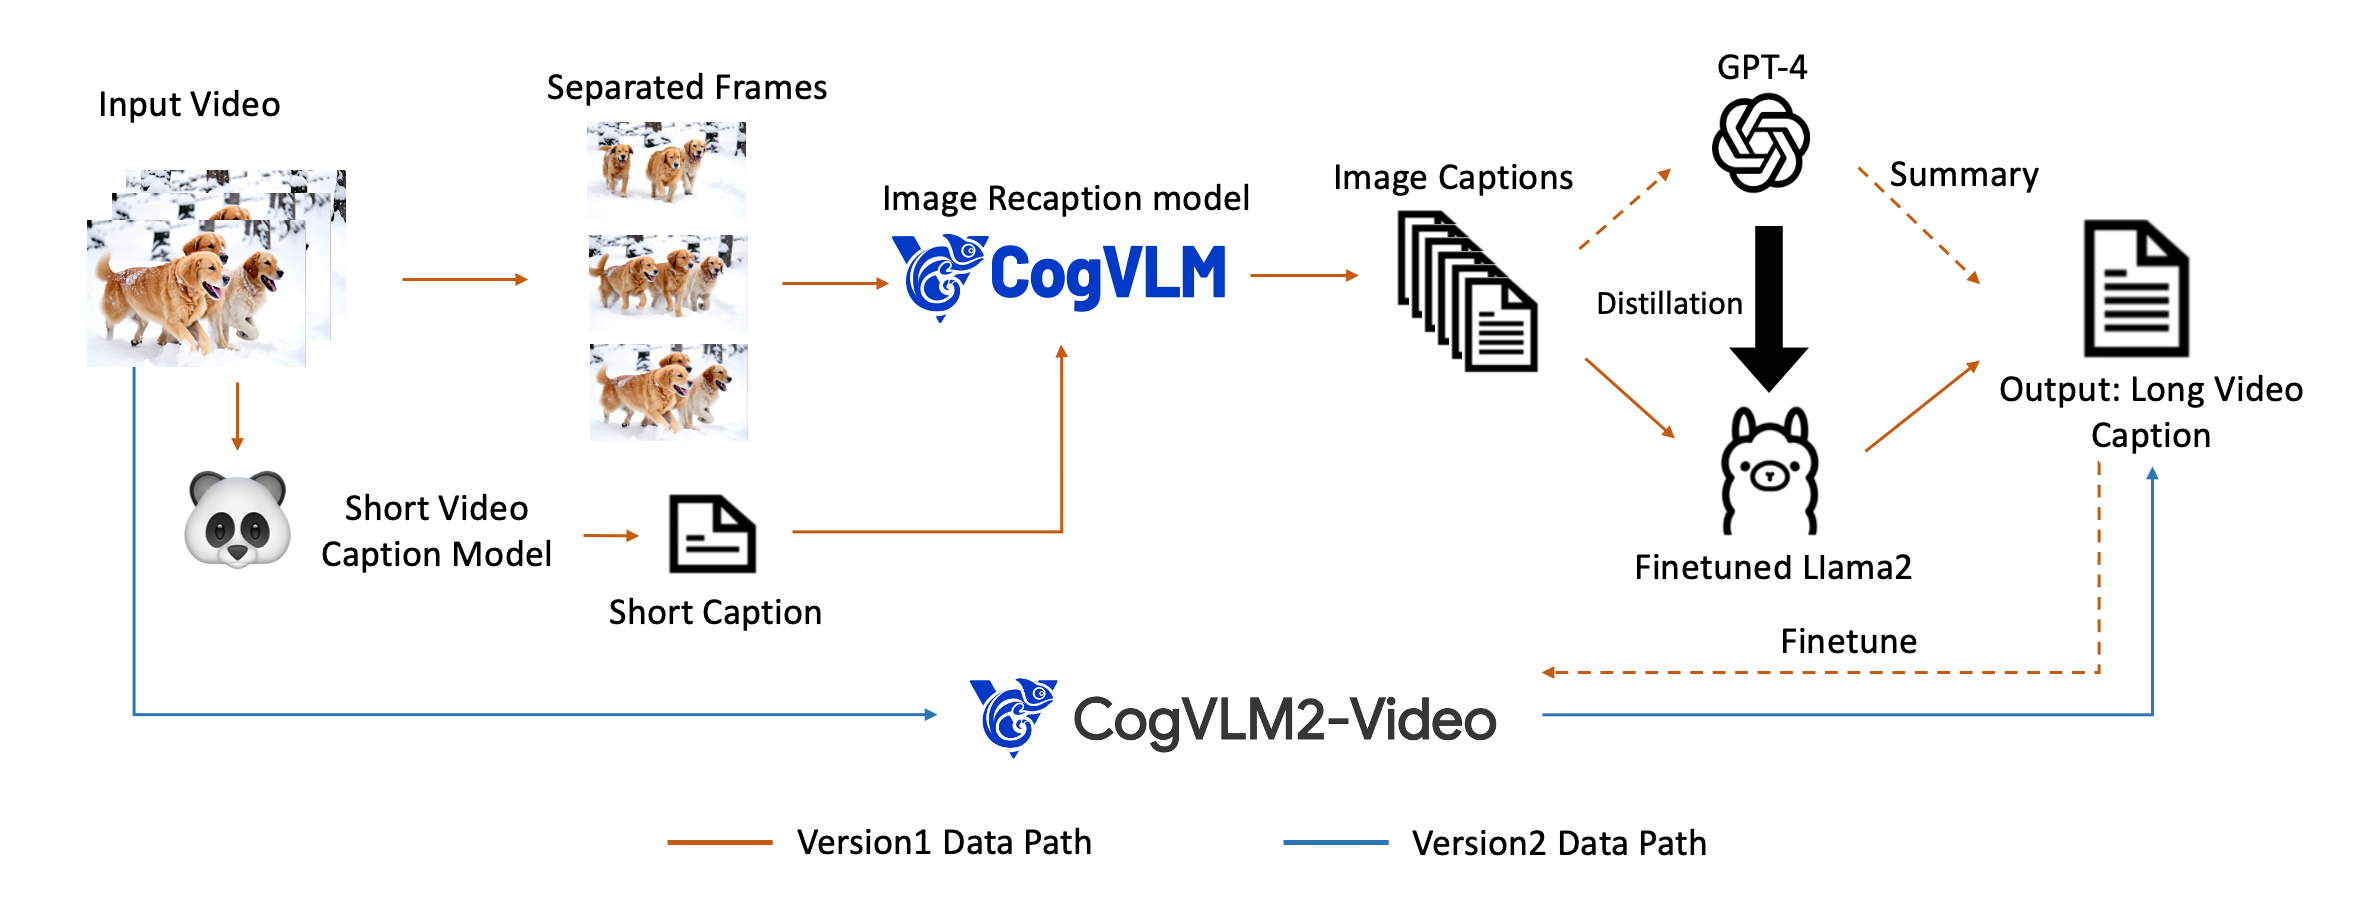
\includegraphics[width=\linewidth]{images/pipeline.jpg}
\end{center}
\caption{The pipeline for dense video caption data generation. In this pipeline, we generate short video captions with the Panda70M model, extract frames to create dense image captions, and use GPT-4 to summarize these into final video captions. To accelerate this process, we fine-tuned a Llama 2 model with the GPT-4 summaries.}
\label{fig:video_caption_gen}
\end{figure}

%\paragraph{.} 
To generate high-quality video caption data, we establish a \textit{Dense Video Caption Data Generation} 
%complex data generation 
pipeline, as detailed in Figure~\ref{fig:video_caption_gen}.  
The idea is to generate video captions from image captions. %

First, we use the Panda70M video captioning model~\citep{chen2024panda} to generate short captions for the videos. 
Then, we employ the image recaptioning model CogVLM~\citep{wang2023cogvlm} used in Stable~Diffusion~3~\citep{esser2024scaling} and CogView3~\citep{zheng2024cogview3} to create dense image captions for each of the frames within a video.  
Subsequently, we use GPT-4 to summarize all the image captions to produce the final video caption. 
To accelerate the generation from image captions to video captions, we fine-tune a Llama2 model~\citep{touvron2023llama} using the summary data generated by GPT-4~\citep{GPT4}, enabling large-scale video caption data generation. Additional details regarding the video caption data generation process can be found in Appendix~\ref{ap:video_caption_gen}.


%We thus propose to build a pipeline to generate video captions from image captions and then fine-tune an end-to-end video captioning model to obtain more dense video captions. 
%Our final video captioning model can generate more detailed descriptions of videos, further enhancing the quality of video generation \citep{betker2023improving}.
 
The pipeline above generates the caption data that is used to trained the \model model introduced in this report. 
To further accelerate video recaptioning, we also fine-tune an end-to-end video understanding model CogVLM2-Caption, based on the CogVLM2-Video\footnote{The CogVLM2-Video model weight is openly available at \url{https://github.com/THUDM/CogVLM2}.} and Llama3~\citep{llama3modelcard}, by using the dense caption data generated from the aforementioned pipeline. 
The video caption data generated by CogVLM2-Caption is used to train the next generation of \model. 
%This dense video captions. % as described above through the pipeline method. 
Examples of video captions generated by this end-to-end CogVLM2-Caption model are shown in Appendix~\ref{ap:video_caption_example}. 
In Appendix~\ref{ap:v2v}, we also present some examples of video generation where a video is first input into CogVLM2-Caption to generate captions, which are then used as input for \model to generate new videos, effectively achieving video-to-video generation.





%%%%%

\section{Ablation}
\begin{figure}[h]
    \centering
    \begin{subfigure}[b]{0.48\textwidth}
        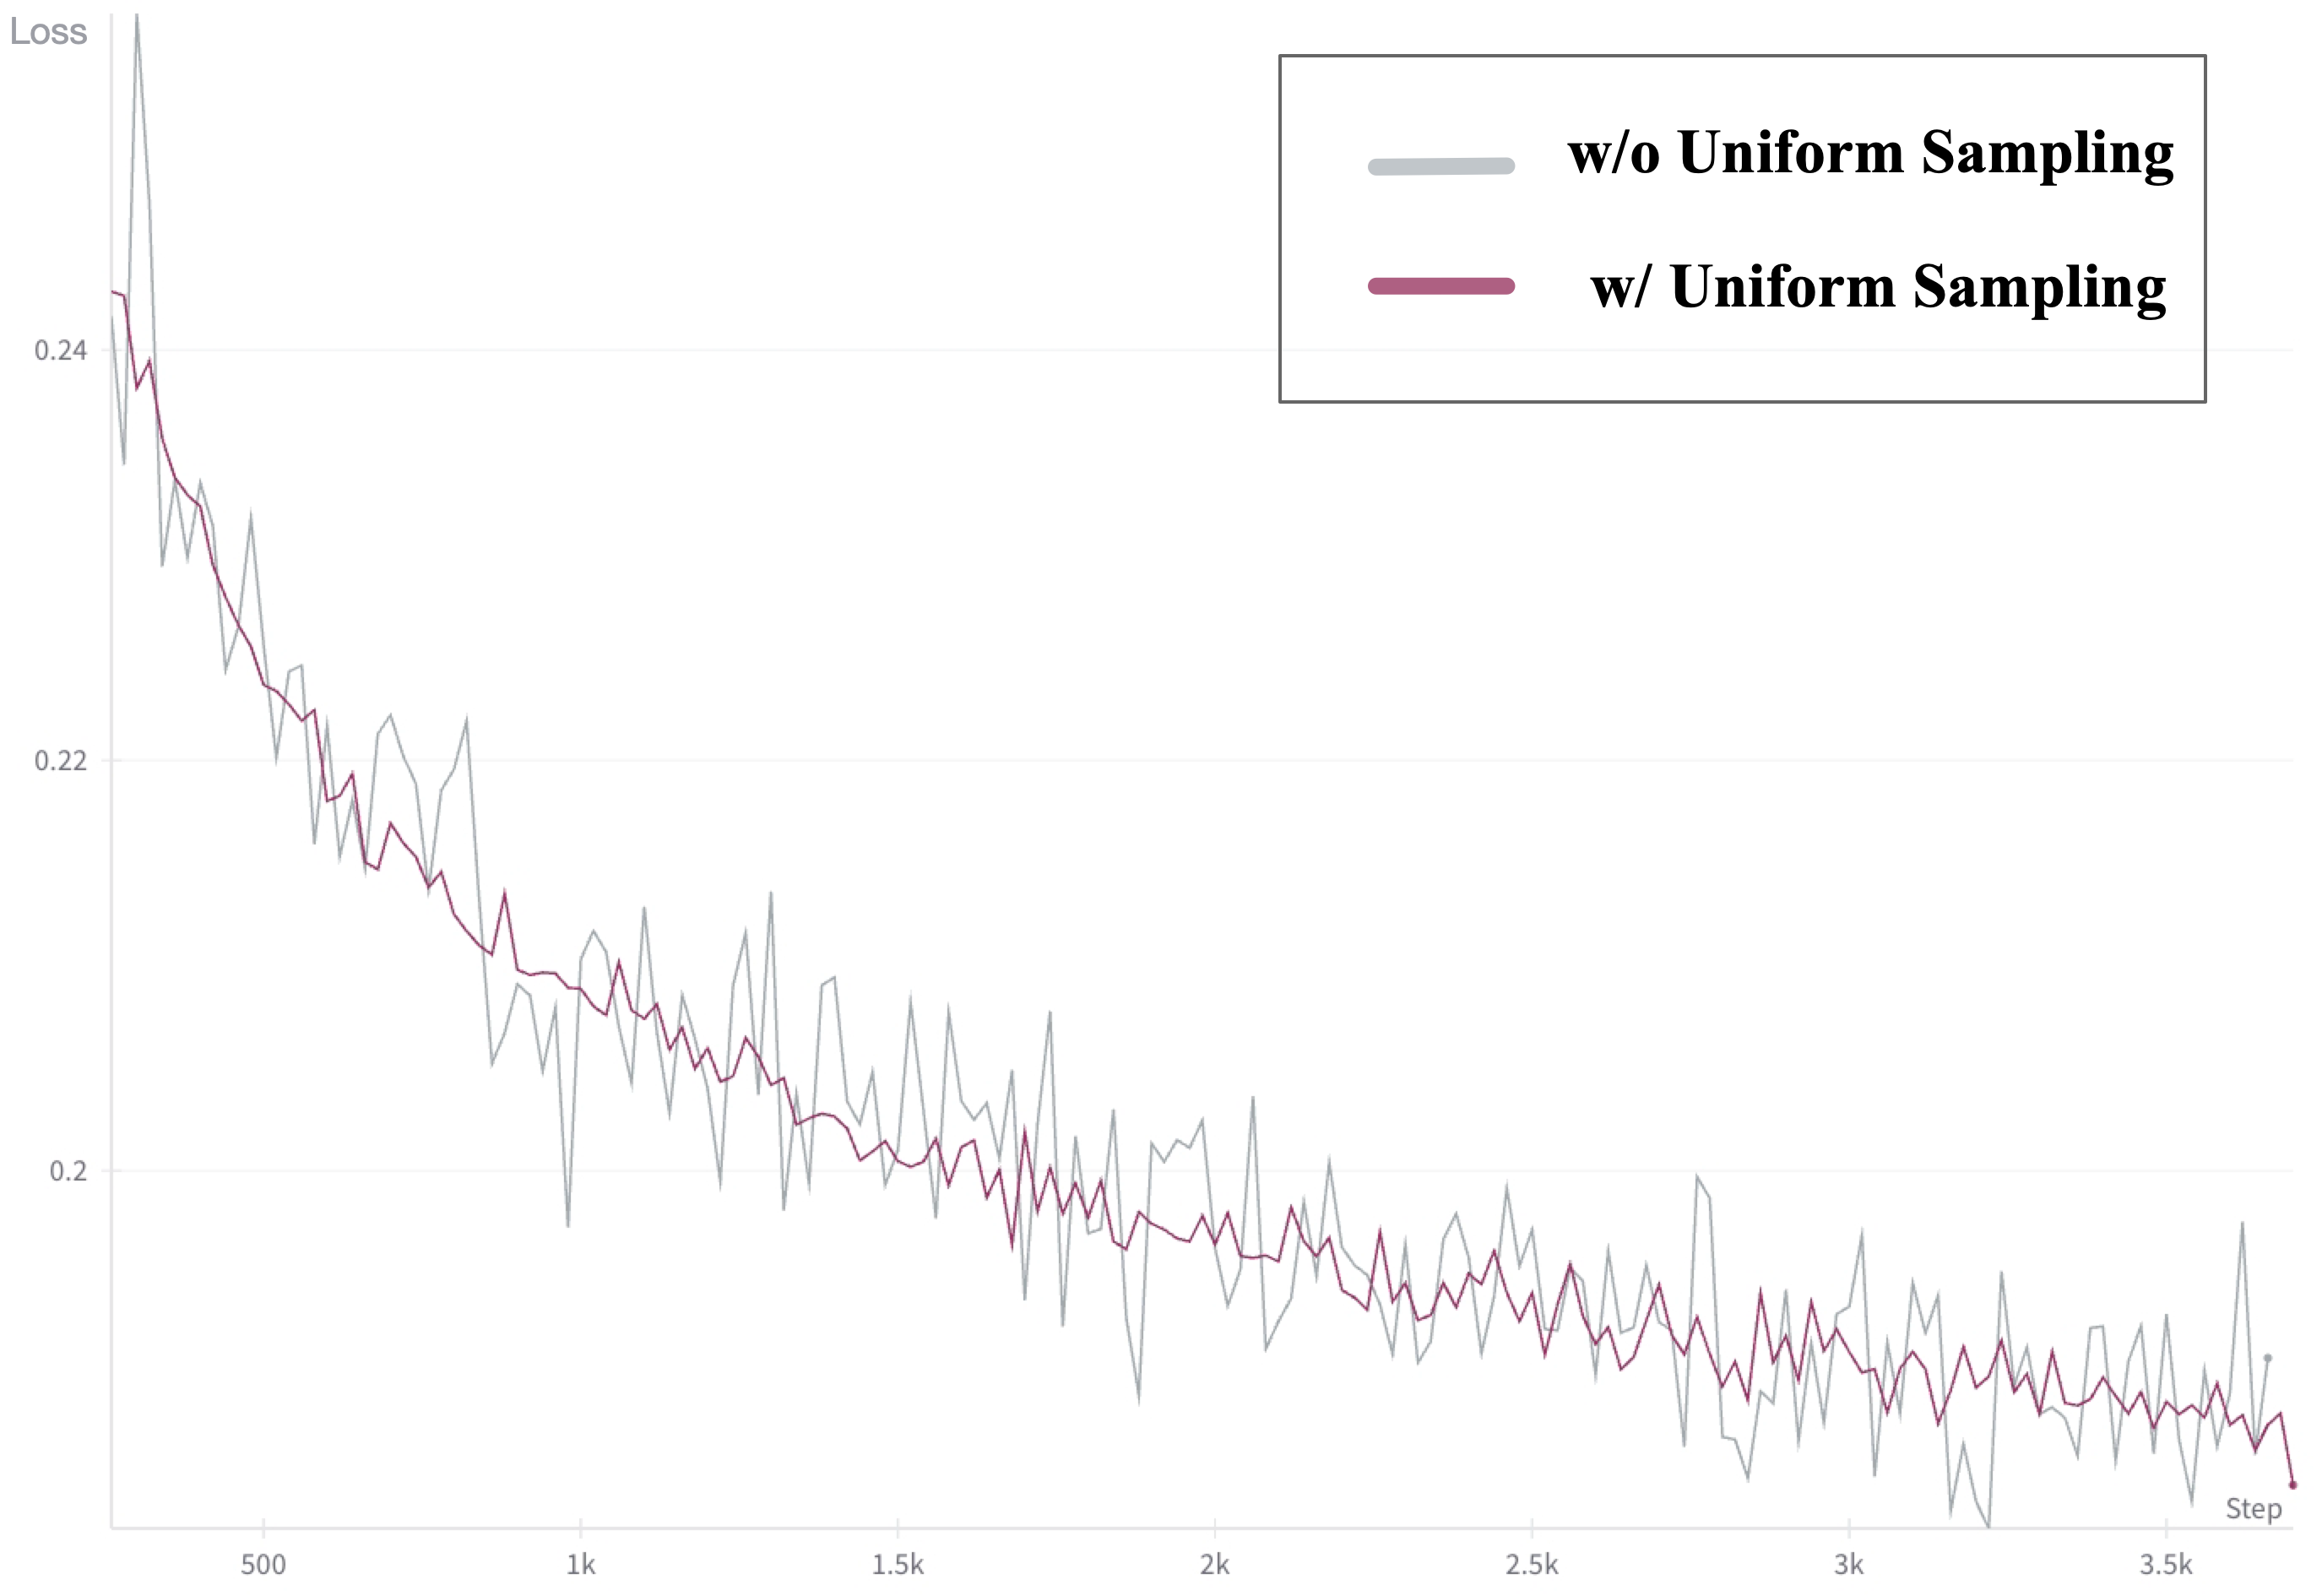
\includegraphics[width=\textwidth]{images/ab_us.png}
        \caption{Bottom aligned}
        \label{fig:a}
    \end{subfigure}
    \begin{subfigure}[b]{0.48\textwidth}
        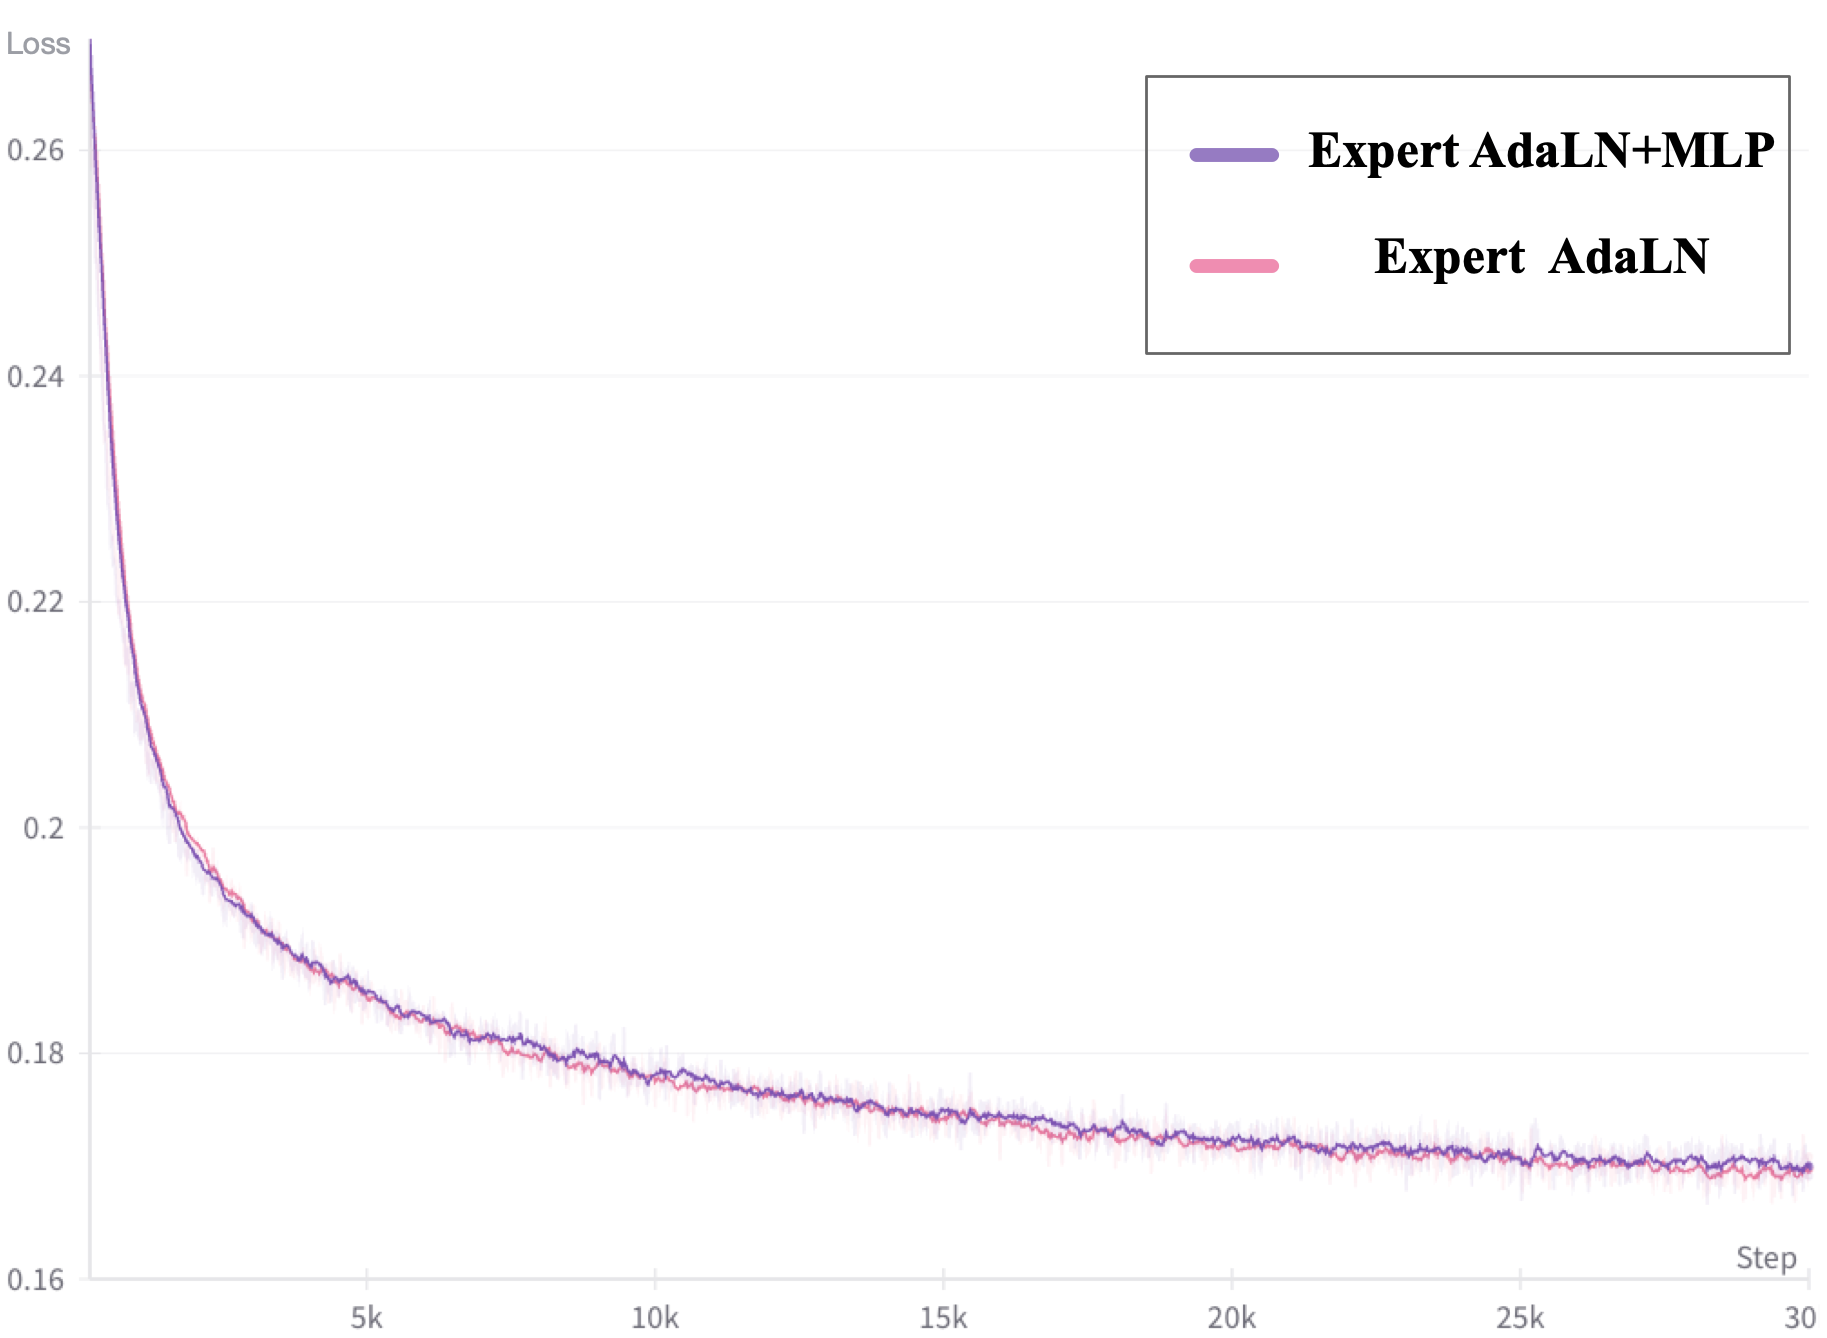
\includegraphics[width=\textwidth]{images/ab_ex.png}
        \caption{Bottom aligned}
        \label{fig:b}
    \end{subfigure}
    \begin{subfigure}[b]{0.50\textwidth}
        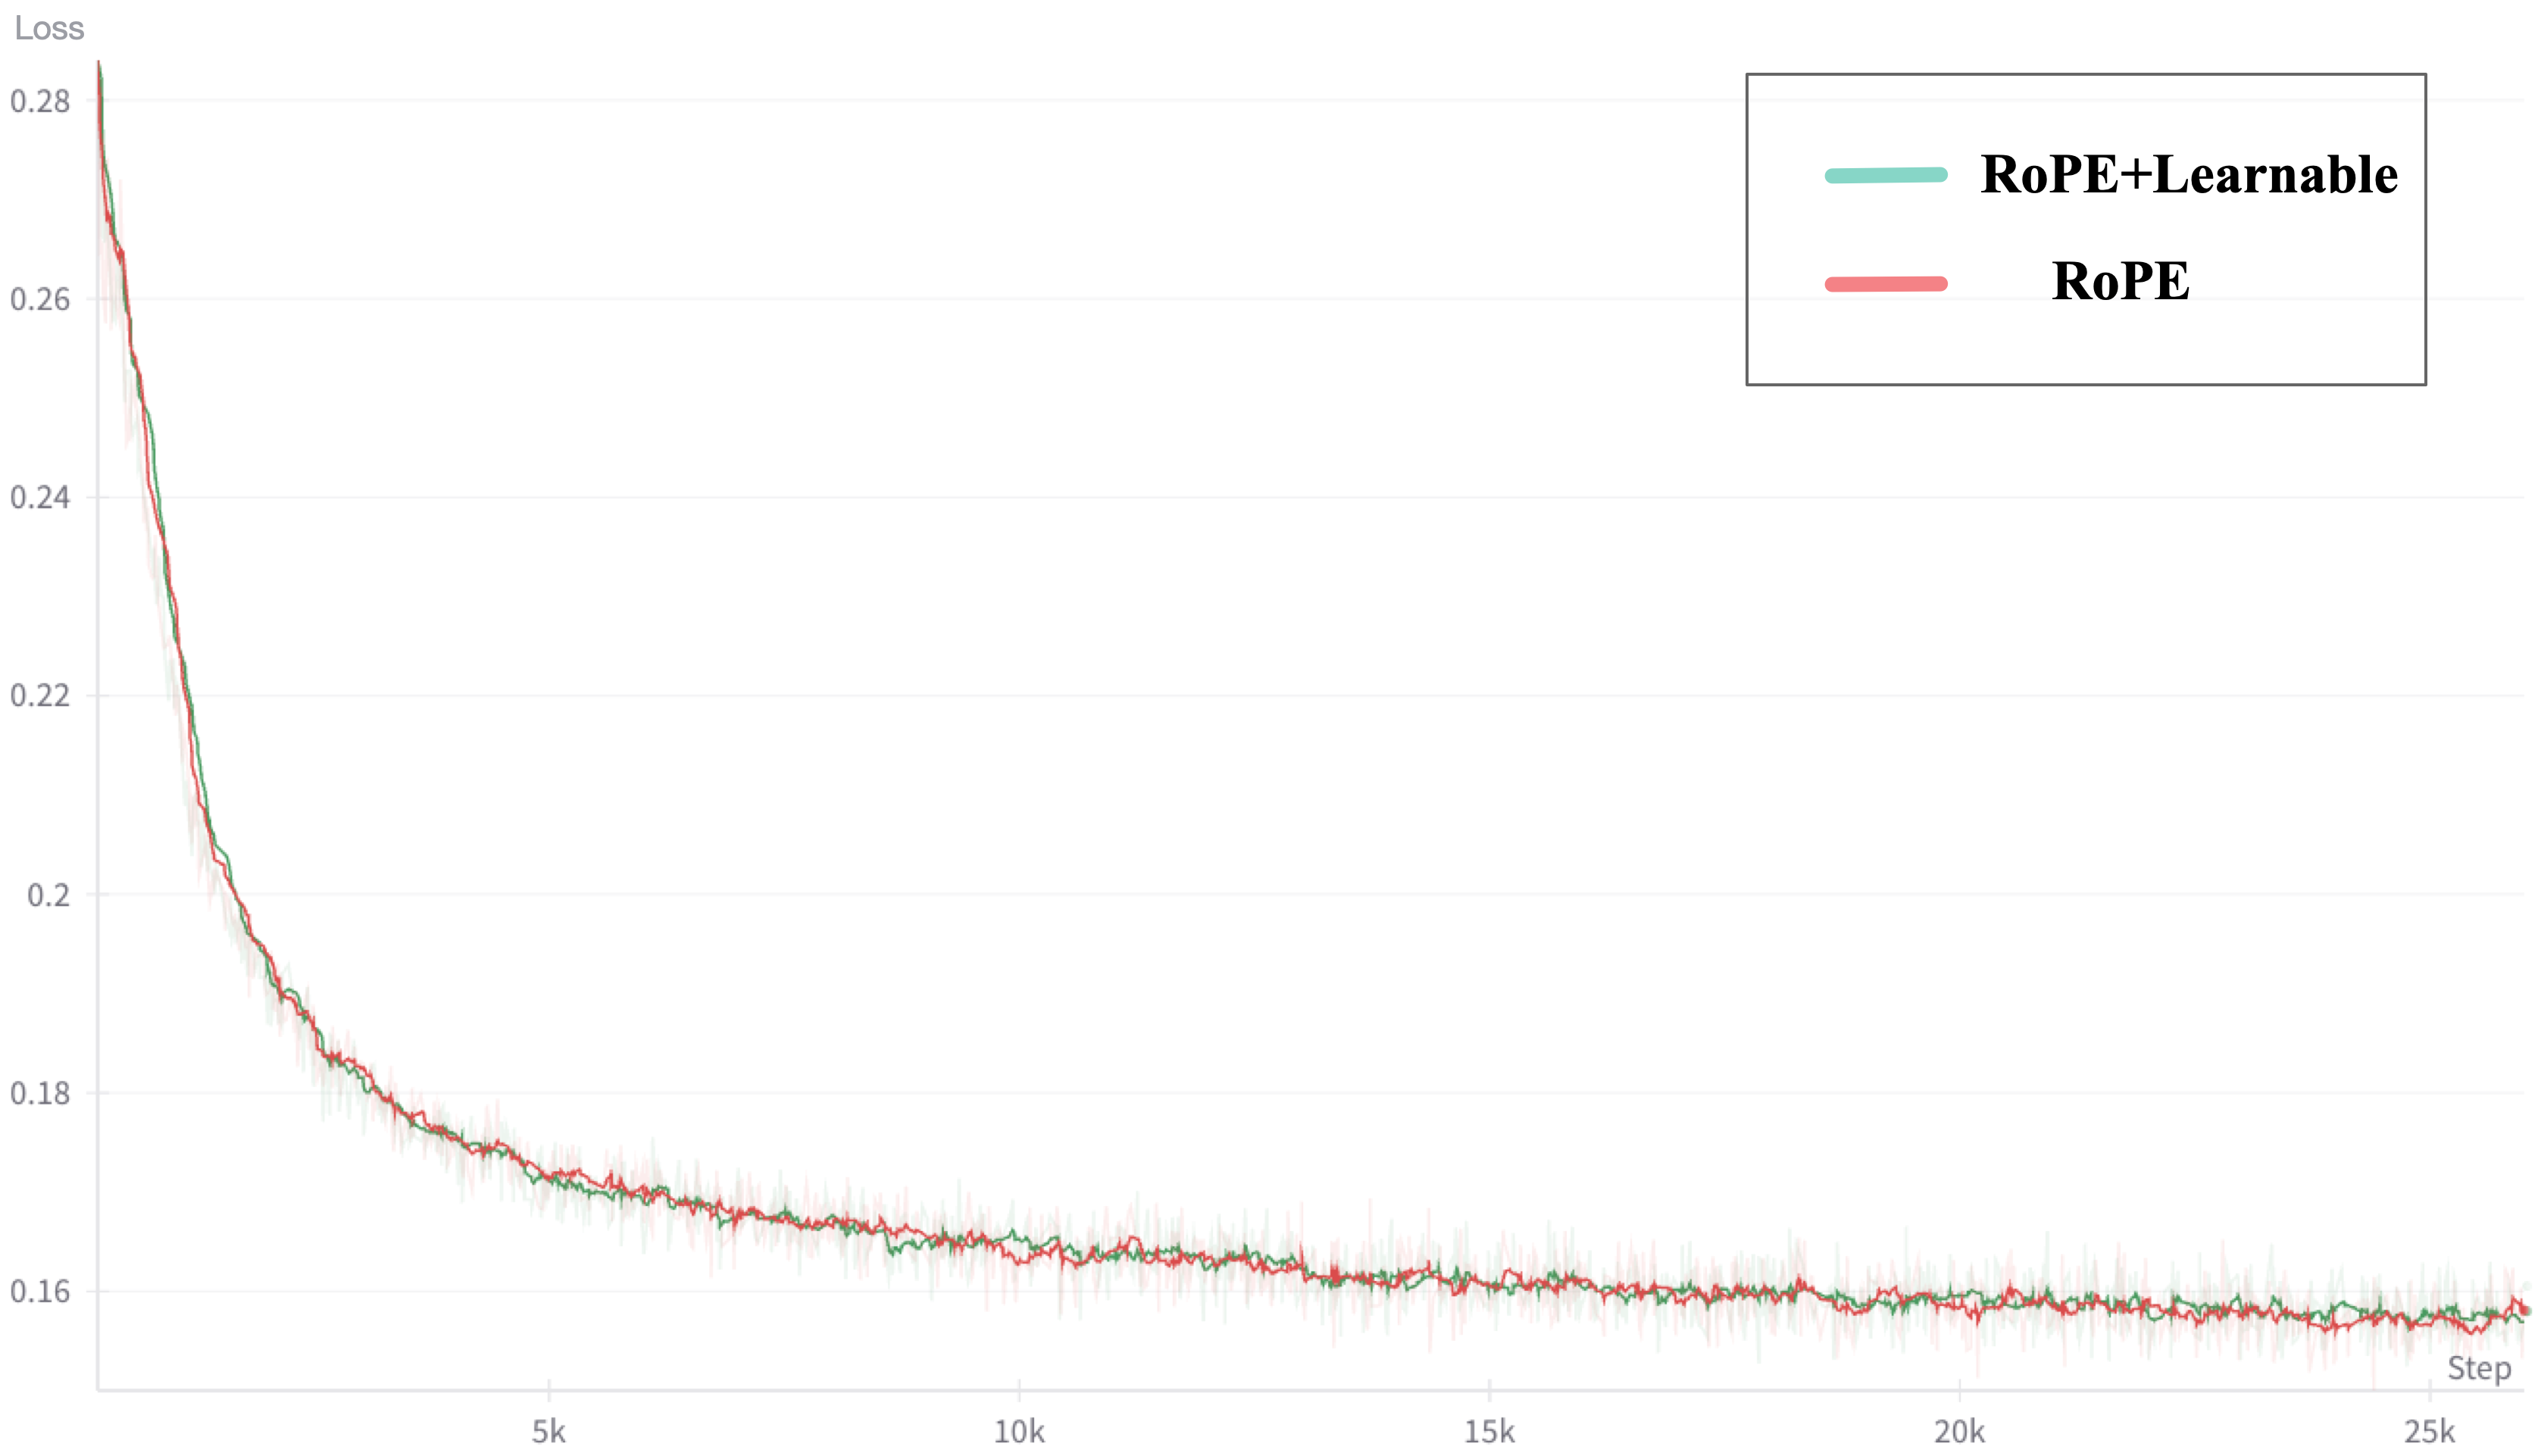
\includegraphics[width=\textwidth]{images/ab_rl.png}
        \caption{Bottom aligned}
        \label{fig:c}
    \end{subfigure}
    \begin{subfigure}[b]{0.46\textwidth}
        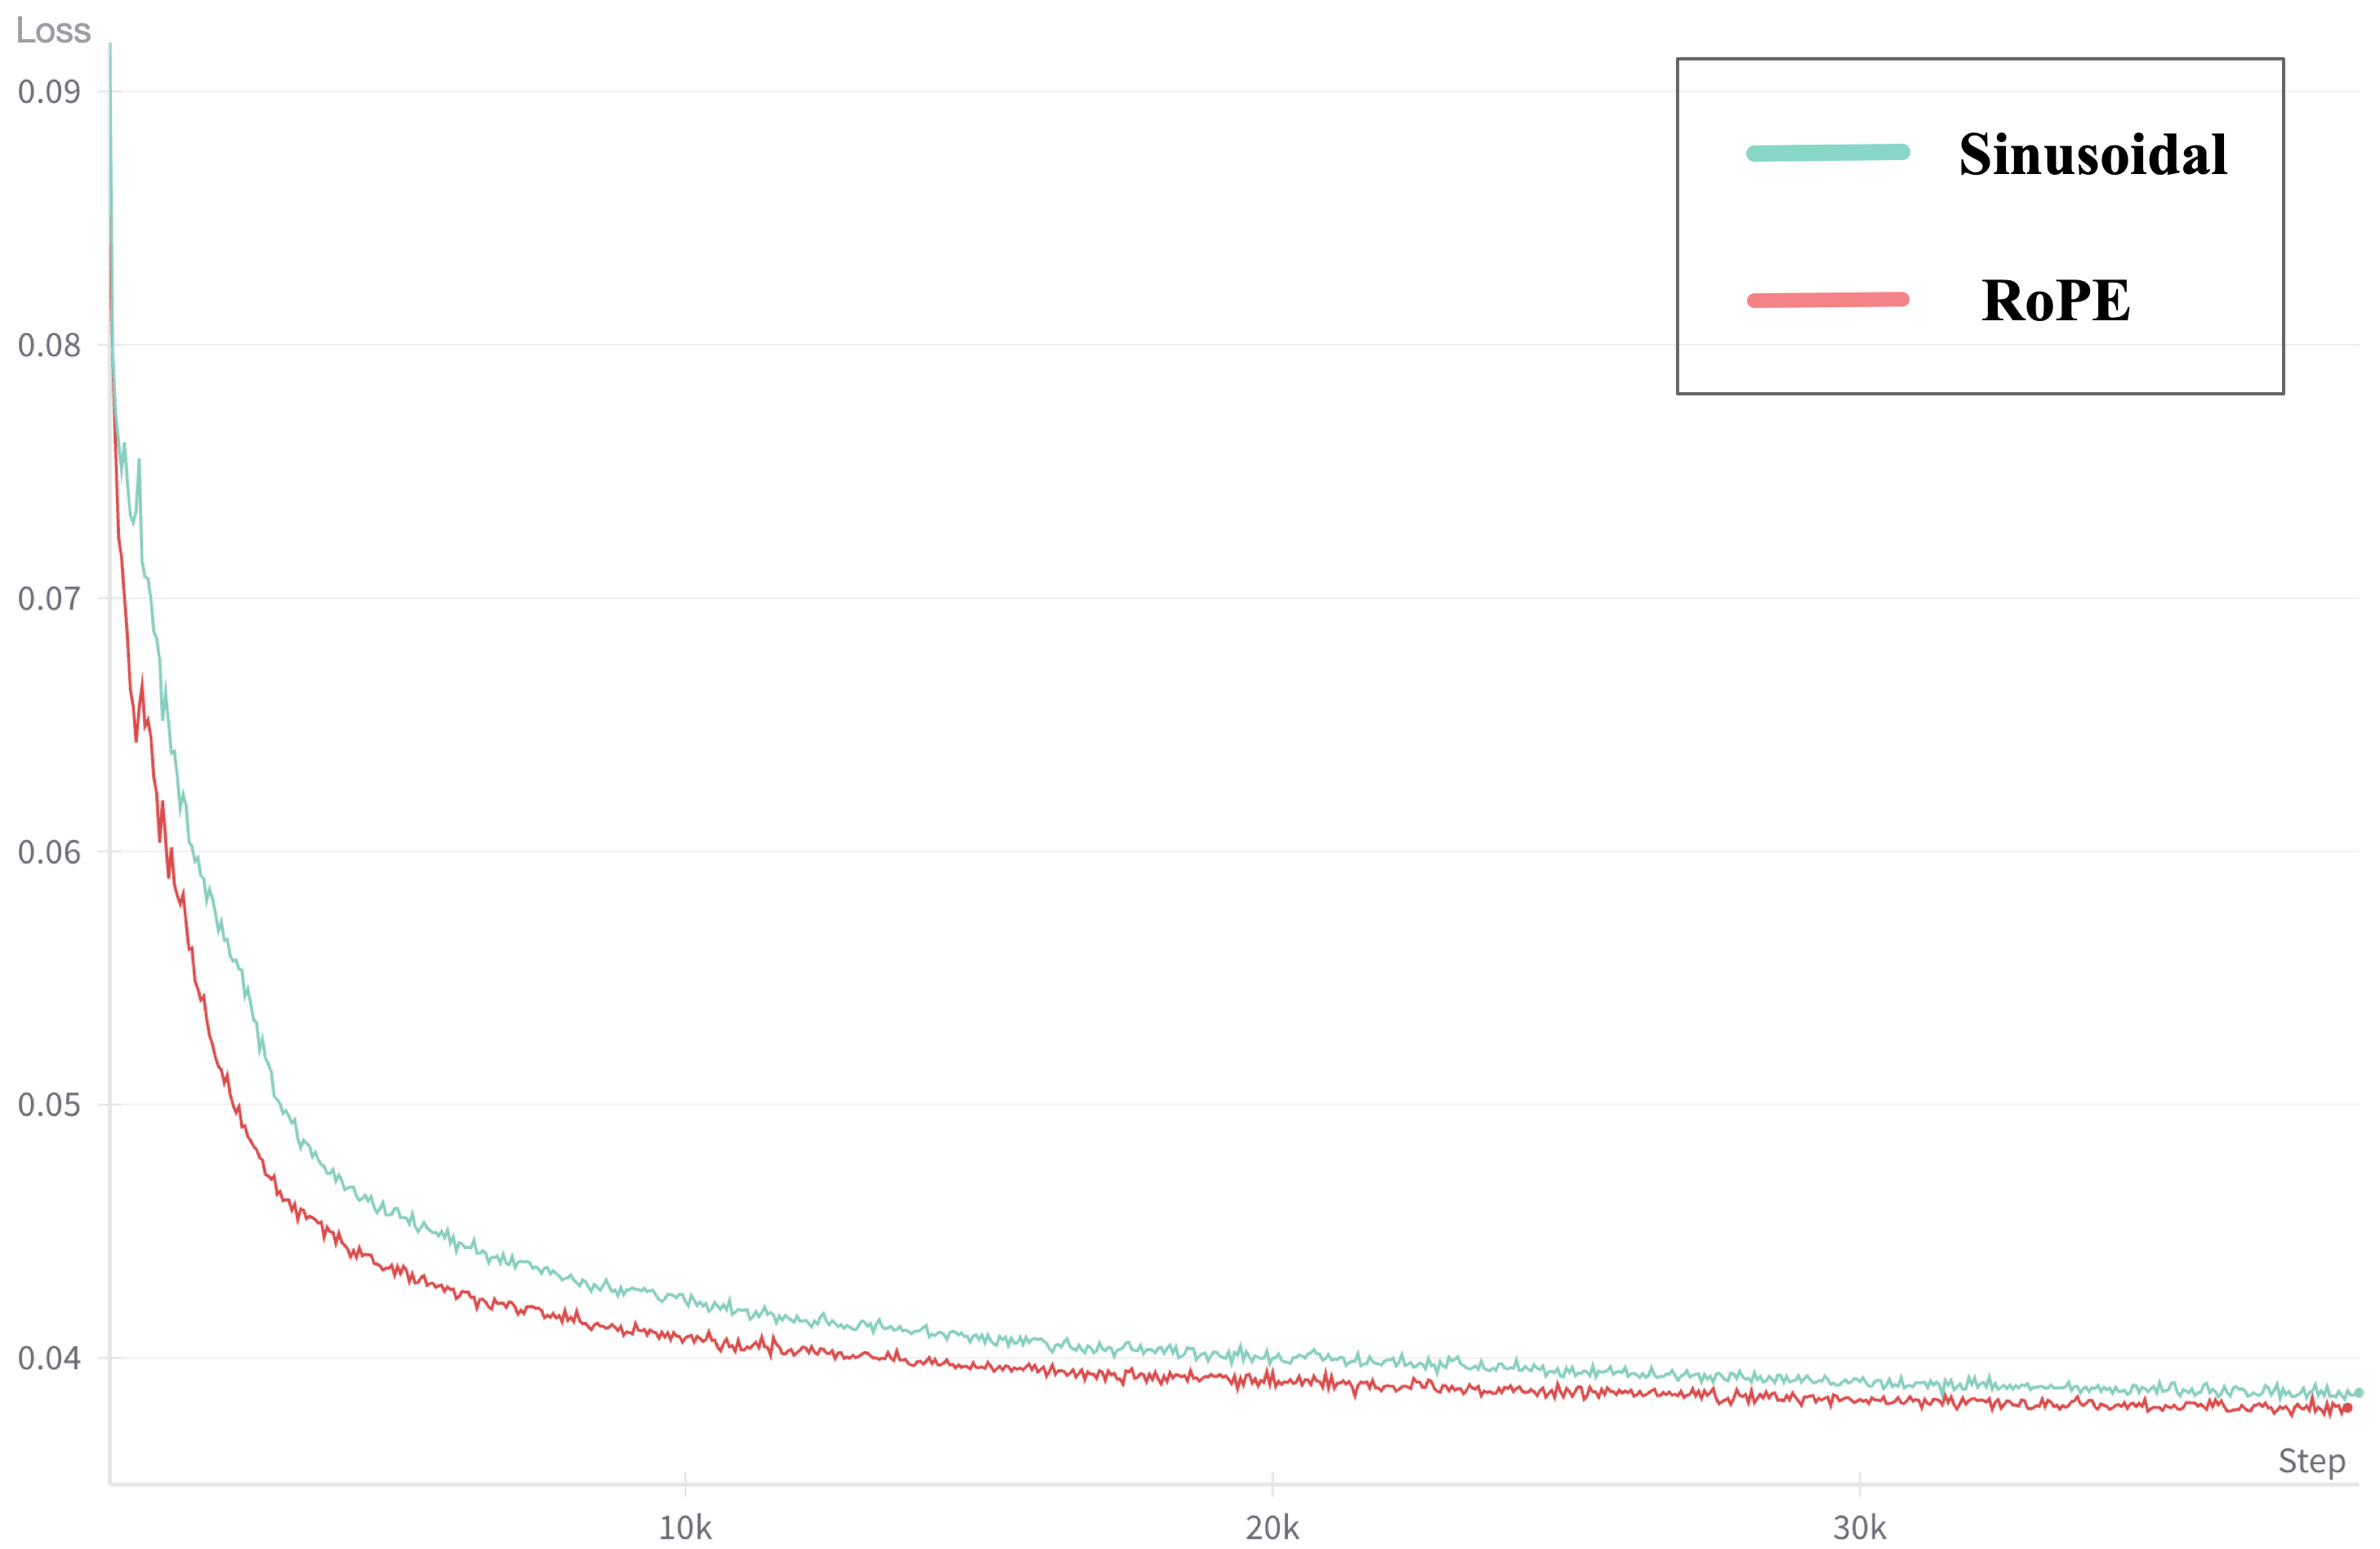
\includegraphics[width=\textwidth]{images/ab_sr.png}
        \caption{Bottom aligned}
        \label{fig:d}
    \end{subfigure}
    \caption{Overall caption for the figure.}
    \label{fig:subfigures}
\end{figure}

We conducted ablation studies on some of the designs mentioned in Section~\ref{sec:model} to verify their effectiveness.


\subsection{Position Embedding}
First, we compared 3D RoPE with sinusoidal absolute position encoding. As shown in Figure~\ref{fig:d}, the loss curve using 3D RoPE converges significantly faster than that with sinusoidal encoding.
Then we compared the use of 3D RoPE alone with the combination of 3D RoPE and learnable absolute position embedding. As shown in Figure~\ref{fig:c}, the loss curves of both methods converge almost identically. For simplicity, we chose to use 3D RoPE alone.

\subsection{Expert Adaptive Layernorm}
We experimented with different ways of incorporating experts: expert LayerNorm and MLP, and expert Layernorm only. Our experiments found that adding expert MLP does not effectively accelerate the model's convergence (Figure~\ref{fig:b}). To reduce the model parameters, we only chose to use expert adaptive Layernorm.

\section{Empirical Evaluation}
We trained a series of models of various sizes. For all subsequent evaluations, we will use the largest model (referred to as CogVideoX).
In this section, we present the experimental validation of CogVideoX through two primary methods: automated metric evaluation and human assessment, providing a thorough analysis of the performance and quality of the generated videos. 
We trained a series of models with different parameter sizes. The following evaluation defaults to using our largest model.

\subsection{Results of Automated Metric Evaluation} 

\paragraph{Baselines.} We chose several top-performing text-to-video models as our baselines for comparison, including T2V-Turbo~\citep{li2024t2v}, AnimateDiff~\citep{guo2023animatediff}, VideoCrafter2~\citep{chen2024videocrafter2}, OpenSora~\citep{opensora}, Show-1~\citep{zhang2023show}, Gen-2~\citep{gen2}, Pika~\citep{pika} and LaVie-2~\citep{wang2023lavie}.



\begin{table}[t]
\caption{Evaluation results.}
\label{table:results}
\vspace{6pt}
\footnotesize
    \centering
    \begin{tabular}{cccccccc}
   \toprule
        Models & \Centerstack{Human \\Action}   & Scene & \Centerstack{Dynamic \\Degree} & \Centerstack{Multiple \\Objects} & \Centerstack{Appearance \\Style} & \Centerstack{Dynamic \\Quality} & \Centerstack{GPT4o-MT \\Score}  \\ 
        \midrule
        T2V-Turbo & 95.2 & \textbf{55.58} & 49.17 & 54.65 & 24.42 & -- & --  \\ 
        AnimateDiff & 92.6  & 50.19 & 40.83 & 36.88 & 22.42 & -- & 2.62  \\ 
        VideoCrafter-2.0 & 95.0  & 55.29 & 42.50 & 40.66 & \textbf{25.13} & 43.6 & 2.68  \\ 
        OpenSora V1.2 & 85.8  & 42.47 & 47.22 & 58.41  & 23.89 & 63.7 & 2.52  \\ 
        Show-1 & 95.6  & 47.03 & 44.44 & 45.47  & 23.06 & 57.7 & --  \\ 
        Gen-2 & 89.2  & 48.91 & 18.89 & 55.47 & 19.34 & 43.6 & 2.62  \\ 
        Pika & 88.0  & 44.80 & 37.22 & 46.69  & 21.89 & 52.1 & 2.48  \\ 
        LaVie-2 & 96.4 & 49.59 & 31.11 & 64.88  & 25.09 & -- & 2.46  \\ 
        \hline
        \textbf{CogVideoX-2B} & 88.0 & 39.94 & \textbf{63.33} & 53.70 & 23.67 & 57.7 & 3.09 \\
        \textbf{CogVideoX-5B} & \textbf{96.8} & 55.44 & 62.22 & \textbf{70.95} & 24.44 & \textbf{69.5} & \textbf{3.36} \\
        \bottomrule
    \end{tabular}
\end{table}
\paragraph{Evaluation Metrics.} To evaluate the text-to-video generation, we employed several metrics from VBench~\citep{huang2023vbench}: \emph{Human Action}, \emph{Scene}, \emph{Dynamic Degree}, \emph{Multiple Objects}, and \emph{Appearance Style}. VBench is a suite of tools designed to automatically assess the quality of generated videos. We have selected certain metrics from VBench, excluding others that do not align with our evaluation needs. For example, the color metric, intended to measure the presence of objects corresponding to specific colors across frames in the generated video, assesses the model's quality by calculating the probability. However, this metric may mislead video generation models that exhibit greater variation, thus we chose not to include it in our evaluation. For longer-generated videos, some models might produce videos with minimal changes between frames to obtain higher scores, but these videos lack rich content. Therefore, a metric for evaluating the dynamism of the video becomes more important. To address this, we employed two video evaluation tools, We also employed the \emph{Dynamic Quality} from Devil~\citep{liao2024evaluationtexttovideogenerationmodels} and \emph{GPT4o-MTScore} from ChronoMagic~\citep{yuan2024chronomagic}, which focus more on the dynamic characteristics of videos. \emph{Dynamic Quality} is defined by the integration of various quality metrics with dynamic scores. This approach mitigates biases arising from negative correlations between video dynamics and video quality, leading to a more thorough assessment of video quality. ChronoMagic, for instance, introduces the \emph{GPT4o-MTScore}, a metric designed to measure the metamorphic amplitude of time-lapse videos, such as those depicting physical, biological, and meteorological changes. This metric is obtained by extracting frames from the generated videos at regular intervals and using GPT-4o~\citep{gpt4o} to score the degree of change, providing a fine-grained assessment of video dynamism. This method ensures a more accurate evaluation of the content's variability over time, countering the potential bias of static frame sequences in scoring.



\paragraph{Results.} Table~\ref{table:results} provides a detailed comparison of the performance of our CogVideoX model with other models. Our model achieved the best performance in 5 out of the 7 metrics and showed competitive results in the remaining 2 metrics. These results demonstrate that our model not only excels in video generation quality but also outperforms previous models in handling various complex dynamic scenes. Additionally, Figure~\ref{fig:radar} presents a radar chart comparing the performance of different models.


\begin{figure}[ht]
\begin{center}
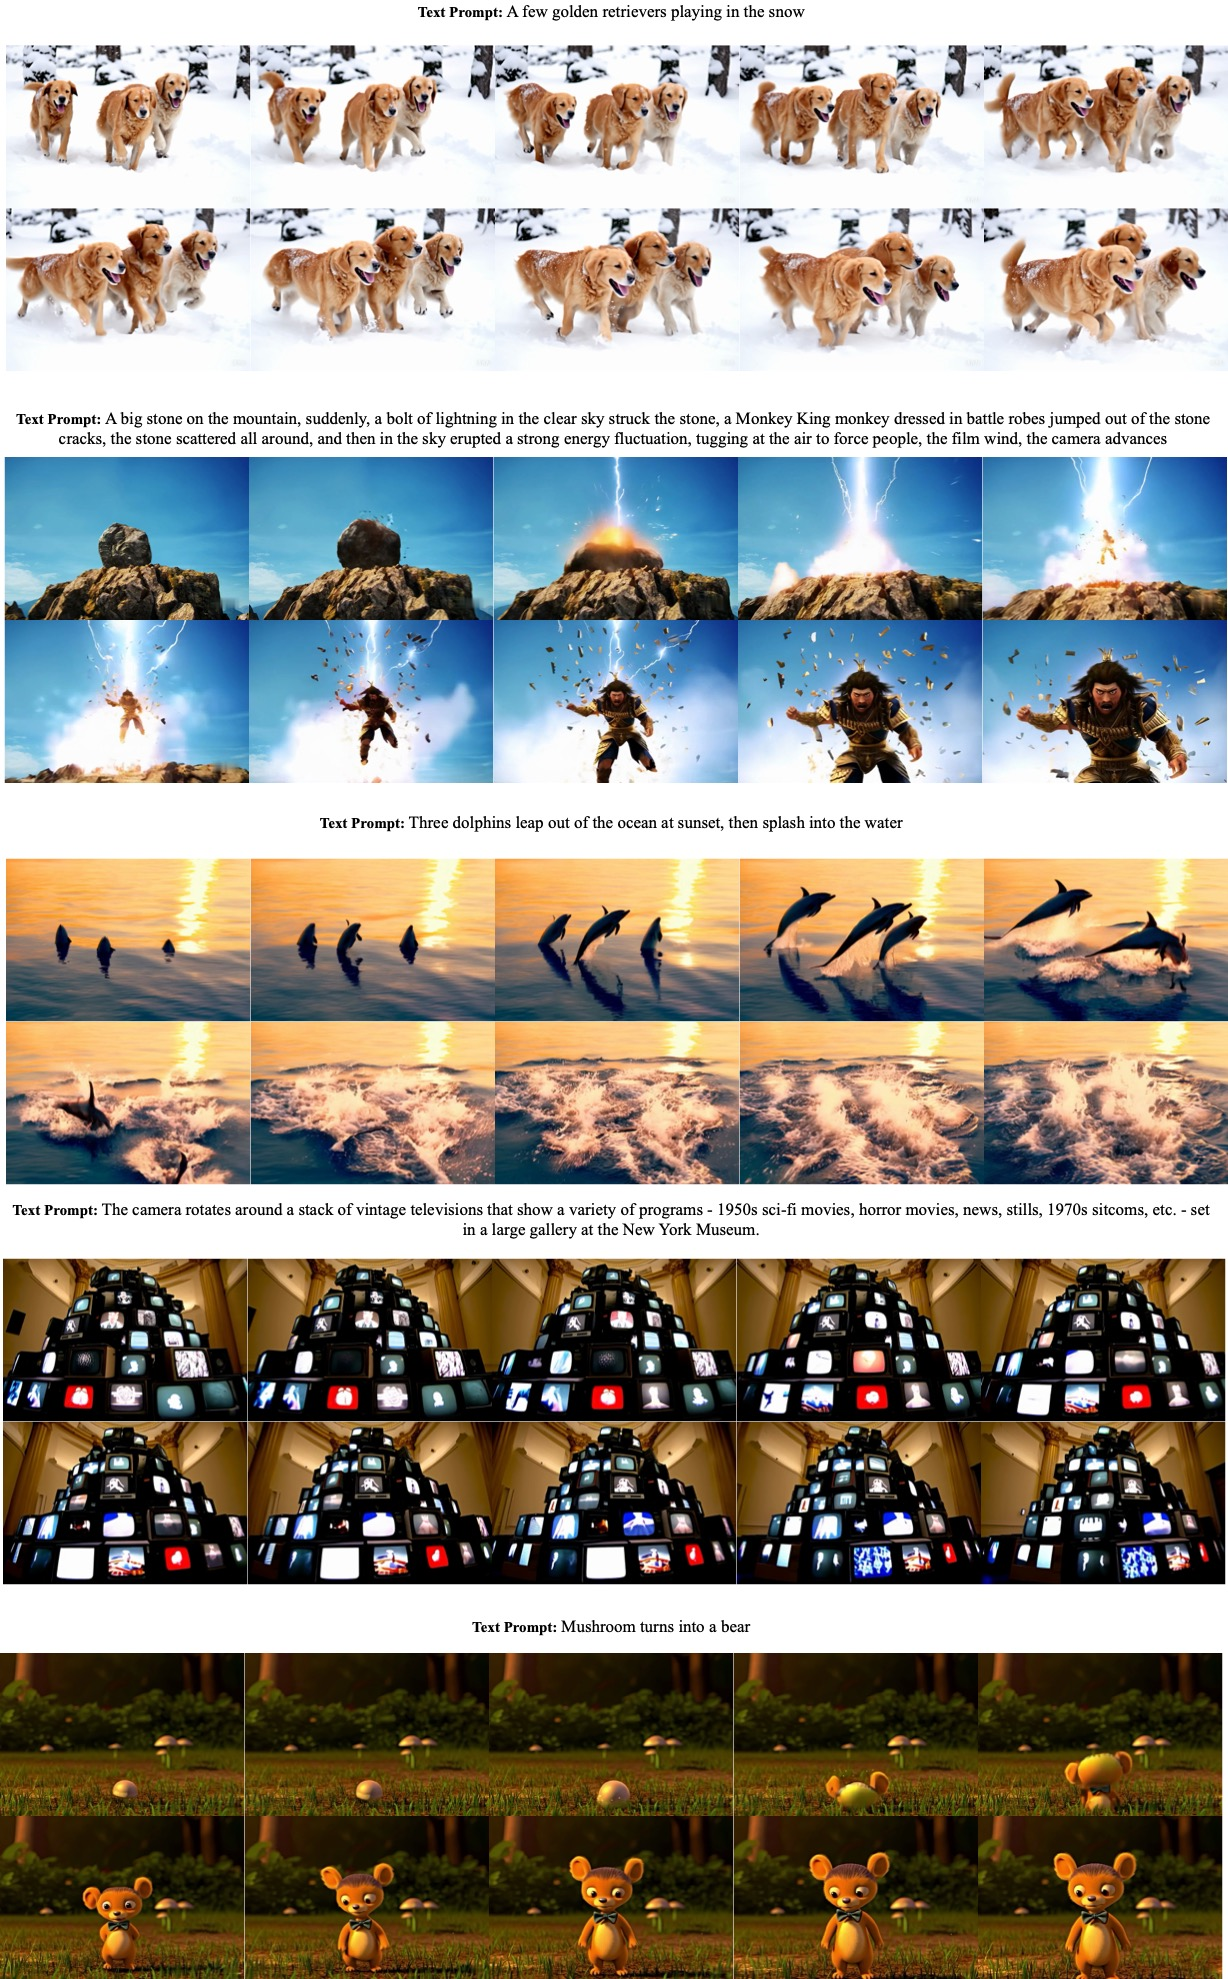
\includegraphics[width=\linewidth]{images/t2v/goodcase1.jpg}
\end{center}
\caption{Text to video showcases. The displayed prompt will be upsampled before being fed into the model. The generated videos contain large motion and can produce various video styles.}
\label{fig:t2vgood1}
\end{figure}

\begin{figure}[ht]
\begin{center}
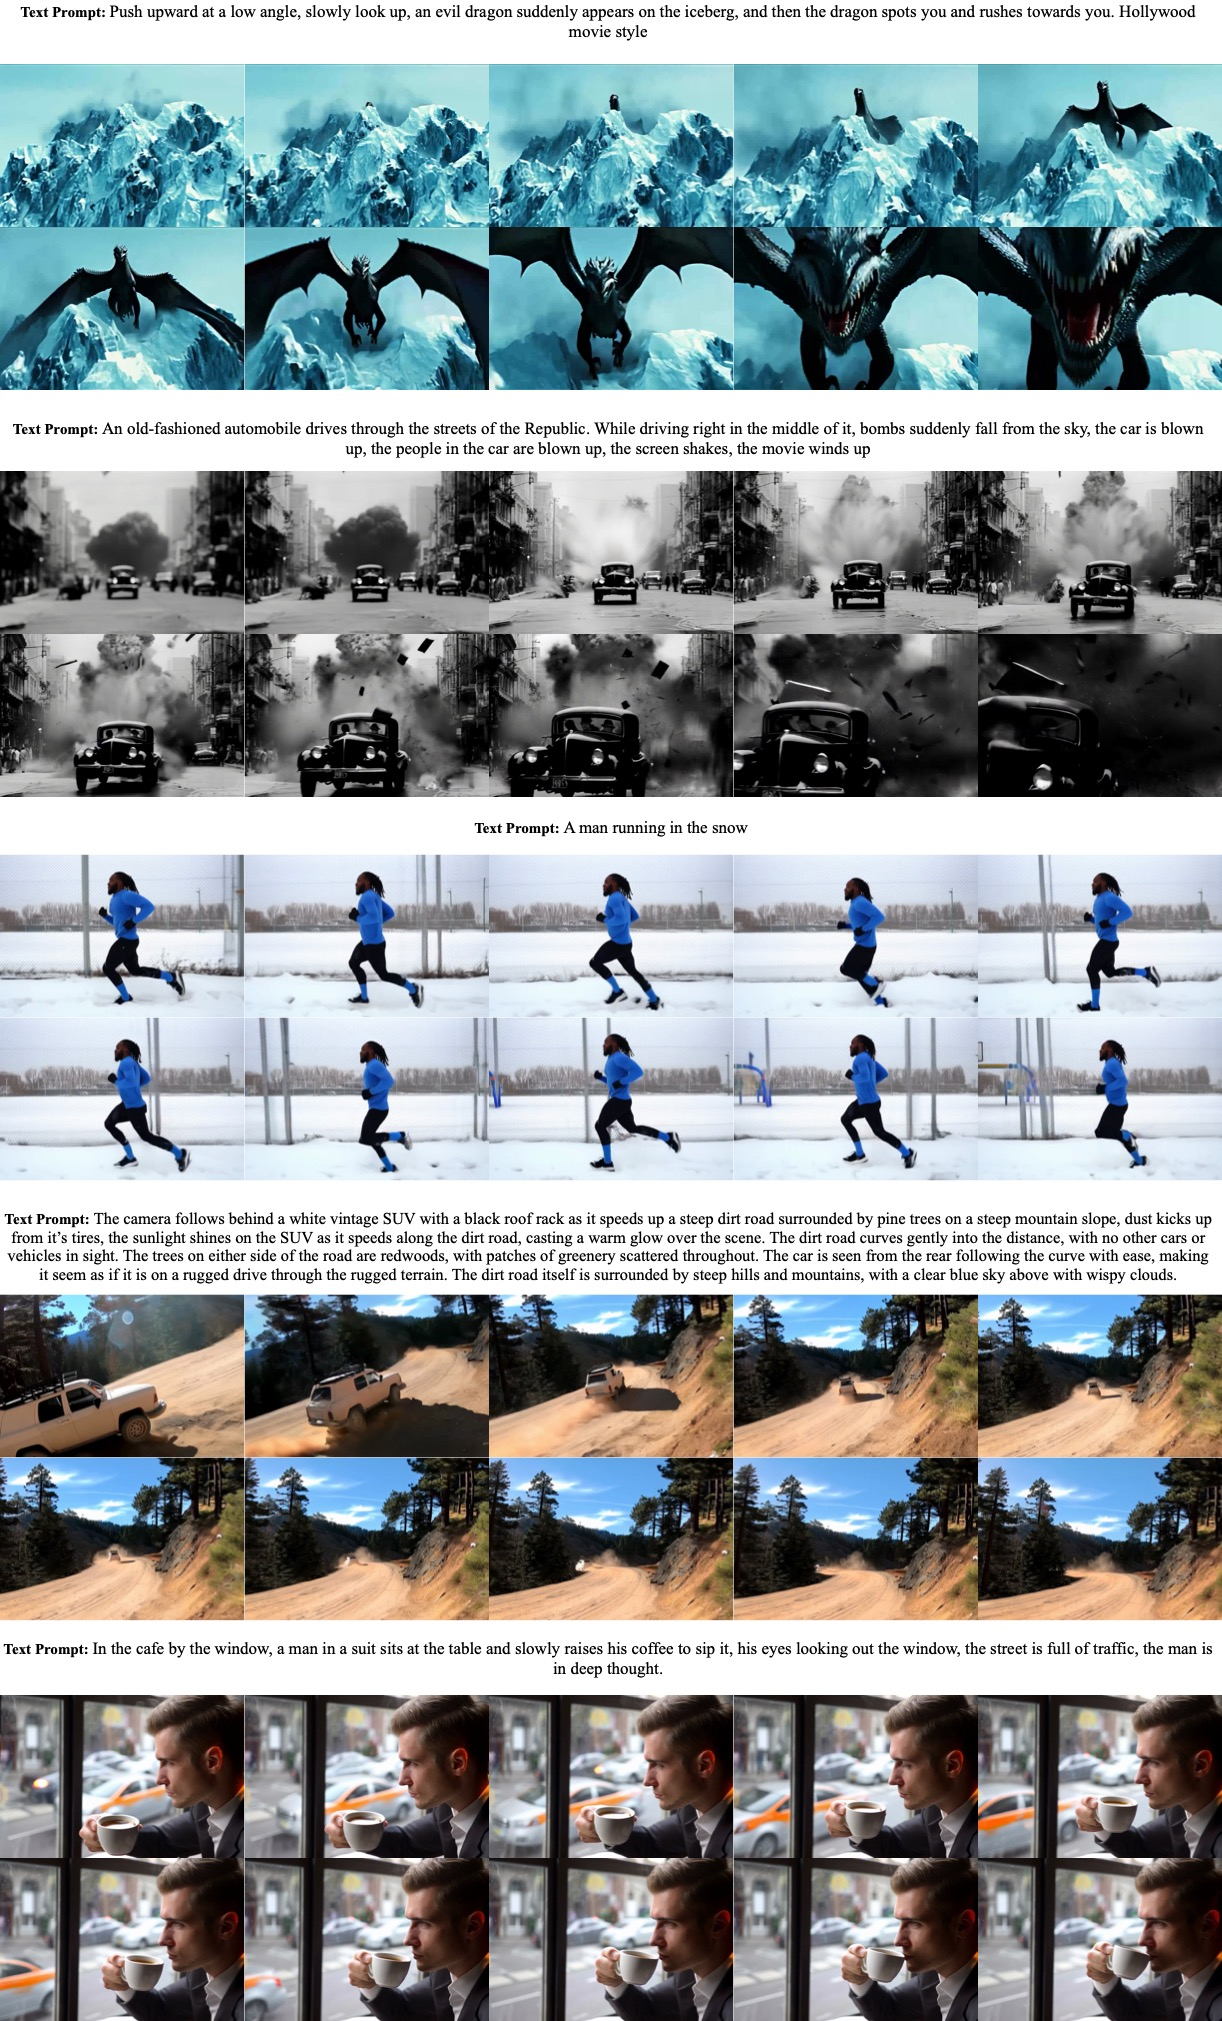
\includegraphics[width=0.98\linewidth]{images/t2v/goodcase2.jpg}
\end{center}
\caption{Text to video showcases.}
\label{fig:t2vgood2}
\end{figure}


% Please add the following required packages to your document preamble:
% \usepackage[table,xcdraw]{xcolor}
% Beamer presentation requires \usepackage{colortbl} instead of \usepackage[table,xcdraw]{xcolor}
% \usepackage[normalem]{ulem}
% \useunder{\uline}{\ul}{}




% \begin{table}[]

% \centering
% \setlength\tabcolsep{3pt}

% \label{sample-table}
% \small
% \vspace{-10pt}
% \caption{\textbf{Automatic Evaluation Results per Dimension.}The table presents a comparative analysis of various video models across different dimensions. It is evident from the table that, in terms of both human motion and background effects as well as the accuracy and distinctiveness of objects, CogVideoX has achieved the current SOTA level. Furthermore, CogVideoX has garnered a commendable score in the expression of dynamic qualities, a capability that serves as a more precise indicator of the intrinsic properties of video media, distinct from the static nature of photographic images.}

% \vspace{6pt}

% \begin{tabular}{cccccccc}
% \toprule
% \multirow{2}{*}{\textbf{Models} }  & \textbf{human}  & \textbf{object} &\multirow{2}{*}{\textbf{scene}}&\textbf{dynamic} &\textbf{multiple} &\textbf{spatial} &\textbf{appearance} \\
%     & \textbf{action}& \textbf{class}& & \textbf{degree} &\textbf{objects}& \textbf{relationship}&\textbf{style}  
% \\
% \midrule
% CogVideoX & 96.80\% &93.70\% & 55.44\% & 62.22\% & 70.95\% & 61.29\% & 24.44\% \\
% {LaVie-2} & 96.40\% & 97.52\%  & 49.59\% & 31.11\% & 64.88\%  & 38.68\% & 25.09\%  \\
% {T2V-Turbo}  & 95.20\%  & 93.96\%& 55.58\% & 49.17\% & 54.65\%    & 38.67\%  & 24.42\%   \\
% {Gen-2}  & 89.20\%& 90.92\%  & 48.91\%  & 18.89\% & 55.47\%    & 66.91\%   & 19.34\%  \\
% {VideoCrafter-2.0\citep{chen2024videocrafter2}} & 95.00\% & 92.55\% & 55.29\%               & 42.50\% & 40.66\% & 35.86\% & 25.13\%  \\
% {Pika Beta} & 88.00\% & 87.45\%  & 44.80\% & 37.22\% & 46.69\% & 65.65\% & 21.89\%   \\
% AnimateDiff-V2 & 92.60\% & 90.90\%  & 50.19\% & 40.83\%        & 36.88\% & 34.60\%  & 22.42\%\\
% {OpenSora V1.2}   & 85.80\% & 83.37\%& 42.47\%   & 47.22\%    & 58.41\% & 67.51\%  & 23.89\%  \\
% {Show-1} & 95.60\%  & 93.07\%  & 47.03\% & 44.44\% & 45.47\% & 53.50\%  & 23.06\%  \\
% {HiGen}  & 86.20\%  & 86.06\%  & 44.88\% & 99.17\% & 22.39\%  & 22.43\% & 24.54\% \\  
% \bottomrule
% \end{tabular}
% \end{table}



% \iffalse



% \begin{table}[ht!]
% \centering
% \caption{Evaluation results.}
% \setlength\tabcolsep{3pt}
% \label{sample-table}
% \begin{center}
% \small
% \resizebox{0.9\linewidth}{!}{
% \begin{tabular}{ccccccccc}

% \multirow{2}{*}{\textbf{Models} }  & \textbf{subject}  & \textbf{background} &\textbf{temporal} &\textbf{motion} &\textbf{dynamic} &\textbf{aesthetic} &\textbf{imaging} &\textbf{object} \\
%     & \textbf{consistency}& \textbf{consistency}& \textbf{flickering}& \textbf{smoothness} &\textbf{degree}& \textbf{quality}&\textbf{quality} & \textbf{class}
% \\ \hline 
%         CogVideoX & 94.66\% & 95.92\% & 97.47\% & 98.10\% & 62.22\% & 55.14\% & 63.62\% & 93.70\%  \\
%         LaVie-2 & 97.90\% & 98.45\% & 98.76\% & 98.42\% & 31.11\% & 67.62\% & 70.39\% & 97.52\%  \\ 
%         T2V-Turbo (VC2) & 96.28\% & 97.02\% & 97.48\% & 97.34\% & 49.17\% & 63.04\% & 72.49\% & 93.96\%  \\ 
%         Gen-2 (2023-06) & 97.61\% & 97.61\% & 99.56\% & 99.58\% & 18.89\% & 66.96\% & 67.42\% & 90.92\%  \\ 
%         VideoCrafter-2.0\citep{chen2024videocrafter2} & 96.85\% & 98.22\% & 98.41\% & 97.73\% & 42.50\% & 63.13\% & 67.22\% & 92.55\%  \\ 
%         Pika Beta (2023-06) & 96.76\% & 98.95\% & 99.77\% & 99.51\% & 37.22\% & 63.15\% & 62.33\% & 87.45\%  \\ 
%         AnimateDiff-V2 & 95.30\% & 97.68\% & 98.75\% & 97.76\% & 40.83\% & 67.16\% & 70.10\% & 90.90\%  \\ 
%         OpenSora V1.2 & 94.45\% & 97.90\% & 99.47\% & 98.20\% & 47.22\% & 56.18\% & 60.94\% & 83.37\%  \\ 
%         Show-1 & 95.53\% & 98.02\% & 99.12\% & 98.24\% & 44.44\% & 57.35\% & 58.66\% & 93.07\%  \\ 
%         HiGen & 90.07\% & 93.99\% & 93.24\% & 96.69\% & 99.17\% & 57.30\% & 63.92\% & 86.06\% \\ 
% \hline \\

% \multirow{2}{*}{\textbf{Models} }  & \textbf{multiple}  & \textbf{human} &\multirow{2}{*}{\textbf{color}} &\textbf{spatial} &\multirow{2}{*}{\textbf{scene}} &\textbf{appearance} &\textbf{temporal} &\textbf{overall} \\
%     & \textbf{objects}& \textbf{action}& & \textbf{relation} & & \textbf{style}&\textbf{style} & \textbf{consistency}
% \\ \hline 
%         CogVideoX & 70.95\% & 96.80\% & 79.75\% & 61.29\% & 55.44\% & 24.44\% & 23.69\% & 26.73\%  \\ 
%         LaVie-2 & 64.88\% & 96.40\% & 91.65\% & 38.68\% & 49.59\% & 25.09\% & 25.24\% & 27.39\%  \\ 
%         T2V-Turbo (VC2) & 54.65\% & 95.20\% & 89.90\% & 38.67\% & 55.58\% & 24.42\% & 25.51\% & 28.16\%  \\
%         Gen-2 (2023-06) & 55.47\% & 89.20\% & 89.49\% & 66.91\% & 48.91\% & 19.34\% & 24.12\% & 26.17\%  \\ 
%         VideoCrafter-2.0 & 40.66\% & 95.00\% & 92.92\% & 35.86\% & 55.29\% & 25.13\% & 25.84\% & 28.23\%  \\
%         Pika Beta (2023-06) & 46.69\% & 88.00\% & 85.31\% & 65.65\% & 44.80\% & 21.89\% & 24.44\% & 25.47\%  \\ 
%         AnimateDiff-V2 & 36.88\% & 92.60\% & 87.47\% & 34.60\% & 50.19\% & 22.42\% & 26.03\% & 27.04\%  \\ 
%         OpenSora V1.2 & 58.41\% & 85.80\% & 87.49\% & 67.51\% & 42.47\% & 23.89\% & 24.55\% & 27.07\%  \\ 
%         Show-1 & 45.47\% & 95.60\% & 86.35\% & 53.50\% & 47.03\% & 23.06\% & 25.28\% & 27.46\%  \\ 
%         HiGen & 22.39\% & 86.20\% & 86.22\% & 22.43\% & 44.88\% & 24.54\% & 25.14\% & 27.14\% \\ \hline

% \hline \\
% \end{tabular}

% }
% \end{center}
% \end{table}

% \fi






% \begin{table}[!ht]
% \centering

% \label{sample-table}
% \small
% \vspace{-10pt}
% \caption{\textbf{Automatic Evaluation Results per Dimension.}}

% \vspace{6pt}

% \resizebox{0.8\linewidth}{!}{
%     \begin{tabular}{cccc}
%         \textbf{Models} & \textbf{\Centerstack{Dynamics Range}} & \textbf{\Centerstack{Dynamics Controllability}} & \textbf{\Centerstack{Dynamics-based Quality}} \\ \hline
%         CogVideoX       & 55.7 & 71.8 & \textbf{69.5} \\ 
%         Gen-2           & 30.8 & \textbf{82.5} & 43.6 \\ 
%         Pika            & 43.2 & 72.0 & 52.1 \\ 
%         VideoCrafter2   & 34.1 & 57.0 & 43.6 \\ 
%         OpenSora        & \textbf{61.2} & 62.4 & 63.7 \\ 
%         Show-1          & 45.1 & 73.9 & 57.7 \\ 
%     \end{tabular}
% }
% \end{table}



\begin{table}[t]
\caption{Evaluation results.}
\label{table:results}
\vspace{6pt}
\footnotesize
    \centering
    \begin{tabular}{cccccccc}
   \toprule
        Models & \Centerstack{Human \\Action}   & Scene & \Centerstack{Dynamic \\Degree} & \Centerstack{Multiple \\Objects} & \Centerstack{Appearance \\Style} & \Centerstack{Dynamic \\Quality} & \Centerstack{GPT4o-MT \\Score}  \\ 
        \midrule
        T2V-Turbo & 95.2 & \textbf{55.58} & 49.17 & 54.65 & 24.42 & -- & --  \\ 
        AnimateDiff & 92.6  & 50.19 & 40.83 & 36.88 & 22.42 & -- & 2.62  \\ 
        VideoCrafter-2.0 & 95.0  & 55.29 & 42.50 & 40.66 & \textbf{25.13} & 43.6 & 2.68  \\ 
        OpenSora V1.2 & 85.8  & 42.47 & 47.22 & 58.41  & 23.89 & 63.7 & 2.52  \\ 
        Show-1 & 95.6  & 47.03 & 44.44 & 45.47  & 23.06 & 57.7 & --  \\ 
        Gen-2 & 89.2  & 48.91 & 18.89 & 55.47 & 19.34 & 43.6 & 2.62  \\ 
        Pika & 88.0  & 44.80 & 37.22 & 46.69  & 21.89 & 52.1 & 2.48  \\ 
        LaVie-2 & 96.4 & 49.59 & 31.11 & 64.88  & 25.09 & -- & 2.46  \\ 
        \hline
        \textbf{CogVideoX-2B} & 88.0 & 39.94 & \textbf{63.33} & 53.70 & 23.67 & 57.7 & 3.09 \\
        \textbf{CogVideoX-5B} & \textbf{96.8} & 55.44 & 62.22 & \textbf{70.95} & 24.44 & \textbf{69.5} & \textbf{3.36} \\
        \bottomrule
    \end{tabular}
\end{table}


\subsection{Human Evaluation}
In addition to automated scoring mechanisms, a comparative analysis between the Kling~\citep{kling} and CogVideoX was conducted using a manual scoring system. One hundred meticulously crafted prompts were used, characterized by their broad distribution, clear articulation, and well-defined conceptual scope. We randomize videos for blind evalution. A panel of evaluators assigned scores for each detail on a scale from zero to one, with the overall total score rated on a scale from zero to five, where higher scores reflect better video quality. Reasons for any score deductions were also carefully documented. The results shown in Table~\ref{table:human_eva} indicate that our model outperforms Kling in all aspects. More details are shown in \ref{sec:human_evalution}.

\begin{table}[!ht]
\centering
\label{sample-table}
\small
\vspace{-5pt}
\caption{Human evaluation between CogVideoX and Kling.}
\label{table:human_eva}
\resizebox{0.75\linewidth}{!}{
    \begin{tabular}{cccccc}
    \toprule
        Model & \Centerstack{Sensory\\Quality} & \Centerstack{Instruction\\Following}&\Centerstack{Physics\\Simulation} & \Centerstack{Cover\\Quality} & 
        \Centerstack{Total\\Score} \\ 
        \midrule
        Kling & 0.638 & 0.367 & 0.561 & 0.668 & 2.17 \\
        \midrule
         {\bf CogVideoX-5B} & {\bf 0.722} & {\bf 0.495} & {\bf 0.667} & {\bf 0.712} & {\bf 2.74}  \\
        \bottomrule
    \end{tabular}
}
\end{table}



% \begin{table}[!ht]
% \centering

% \label{sample-table}
% \small
% \vspace{-10pt}
% \caption{\textbf{Automatic Evaluation Results per Dimension.}}

% \vspace{6pt}

% \resizebox{0.8\linewidth}{!}{
%     \begin{tabular}{cccc}
%         \textbf{Models} & \textbf{\Centerstack{Dynamics Range}} & \textbf{\Centerstack{Dynamics Controllability}} & \textbf{\Centerstack{Dynamics-based Quality}} \\ \hline
%         CogVideoX       & 55.7 & 71.8 & \textbf{69.5} \\ 
%         Gen-2           & 30.8 & \textbf{82.5} & 43.6 \\ 
%         Pika            & 43.2 & 72.0 & 52.1 \\ 
%         VideoCrafter2   & 34.1 & 57.0 & 43.6 \\ 
%         OpenSora        & \textbf{61.2} & 62.4 & 63.7 \\ 
%         Show-1          & 45.1 & 73.9 & 57.7 \\ 
%     \end{tabular}
% }
% \end{table}




\section{Conclusion}

In this paper, we present CogVideoX, a state-of-the-art text-to-video diffusion model. 
It leverages a 3D VAE and an Expert Transformer architecture to generate coherent long-duration videos with significant motion. 
By implementing a comprehensive data processing pipeline and a video re-captioning method, we significantly improve the quality and semantic alignment of the generated videos. 
Our progressive training techniques, including mixed-duration training and resolution progressive training, further enhance the model's performance and stability. 
Our ongoing efforts focus on refining the \model's ability to capture complex dynamics and ensure even higher quality in video generation. 
We are also exploring the scaling laws of video generation models and aim to train larger and more powerful models to generate longer and higher-quality videos, pushing the boundaries of what is achievable in text-to-video generation. 


 
\subsubsection*{Acknowledgments}
%This research was supported by Zhipu AI. Thanks to BiliBili for data support. Thanks to all our collaborators and partners from Knowledge Engineering Group (KEG) and Zhipu AI.

% We would like to thank Xiaohan Zhang, Da Yin, Guanyu Feng, Ting Liu, Wei Jia, Jiajun Xu and all the data annotators, infra-operating staff, collaborators, and partners as well as everyone at Zhipu AI and Tsinghua University not explicitly mentioned in the report who have provided support, feedback, and contributed to the \model.
We would like to thank all the data annotators, infrastructure operators, collaborators, and partners. We also extend our gratitude to everyone at Zhipu AI and Tsinghua University who have provided support, feedback, or contributed to the \model, even if not explicitly mentioned in this report.
We would also like to greatly thank BiliBili for technical discussions. 
% We would also like to greatly thank BiliBili for data support. 
% We would also like to thank Yuxuan Zhang and Wei Jia from Zhipu AI as well as the teams at Hugging Face, ModelScope, WiseModel, and others for their help on the open-sourcing efforts of the GLM family of models.


% \section*{References}
\bibliography{reference}
\bibliographystyle{iclr2024_conference}


%%%%%%%%%%%%%%%%%%%%%%%%%%%%%%%%%%%%%%%%%%%%%%%%%%%%%%%%%%%%

\clearpage
\appendix
\section{Image To Video Model}
We finetune an image-to-video model from the text-to-video model. Drawing from the \citep{blattmann2023stable}, we add an image as an additional condition alongside the text. The image is passed through 3D VAE and concatenated with the noised input in the channel dimension. Similar to super-resolution tasks, there is a significant distribution gap between training and inference( the first frame of videos vs. real-world images). To enhance the model's robustness, we add large noise to the image condition during training. Some examples are shown in \ref{fig:i2vgood1}, \ref{fig:i2vgood2}. CogVideoX can handle different styles of image input.

\begin{figure}[ht]
\begin{center}
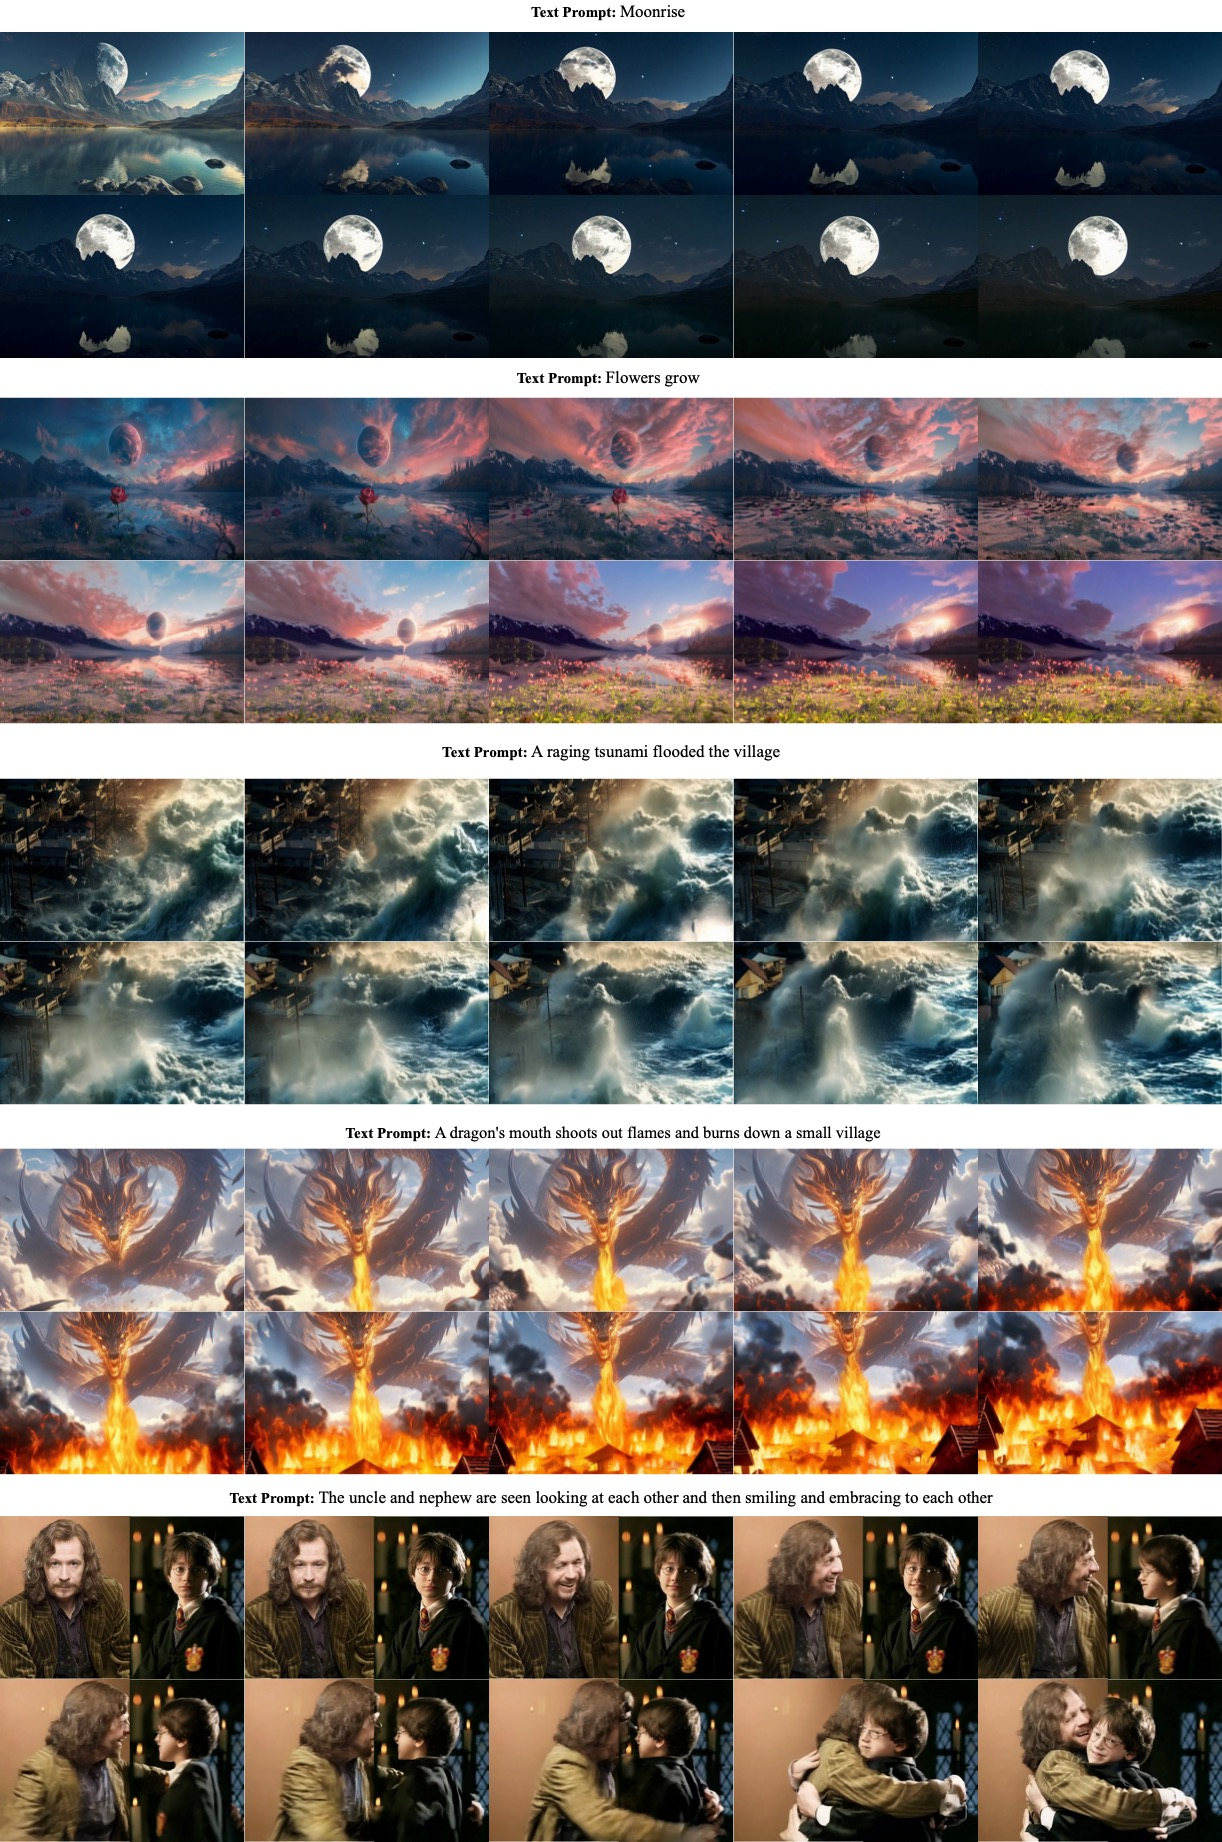
\includegraphics[width=\linewidth]{images/t2v/i2vgood1.jpg}
\end{center}
\caption{Image to video showcases. The displayed prompt will be upsampled before being fed into the model.}
\label{fig:i2vgood1}
\end{figure}

\begin{figure}[ht]
\begin{center}
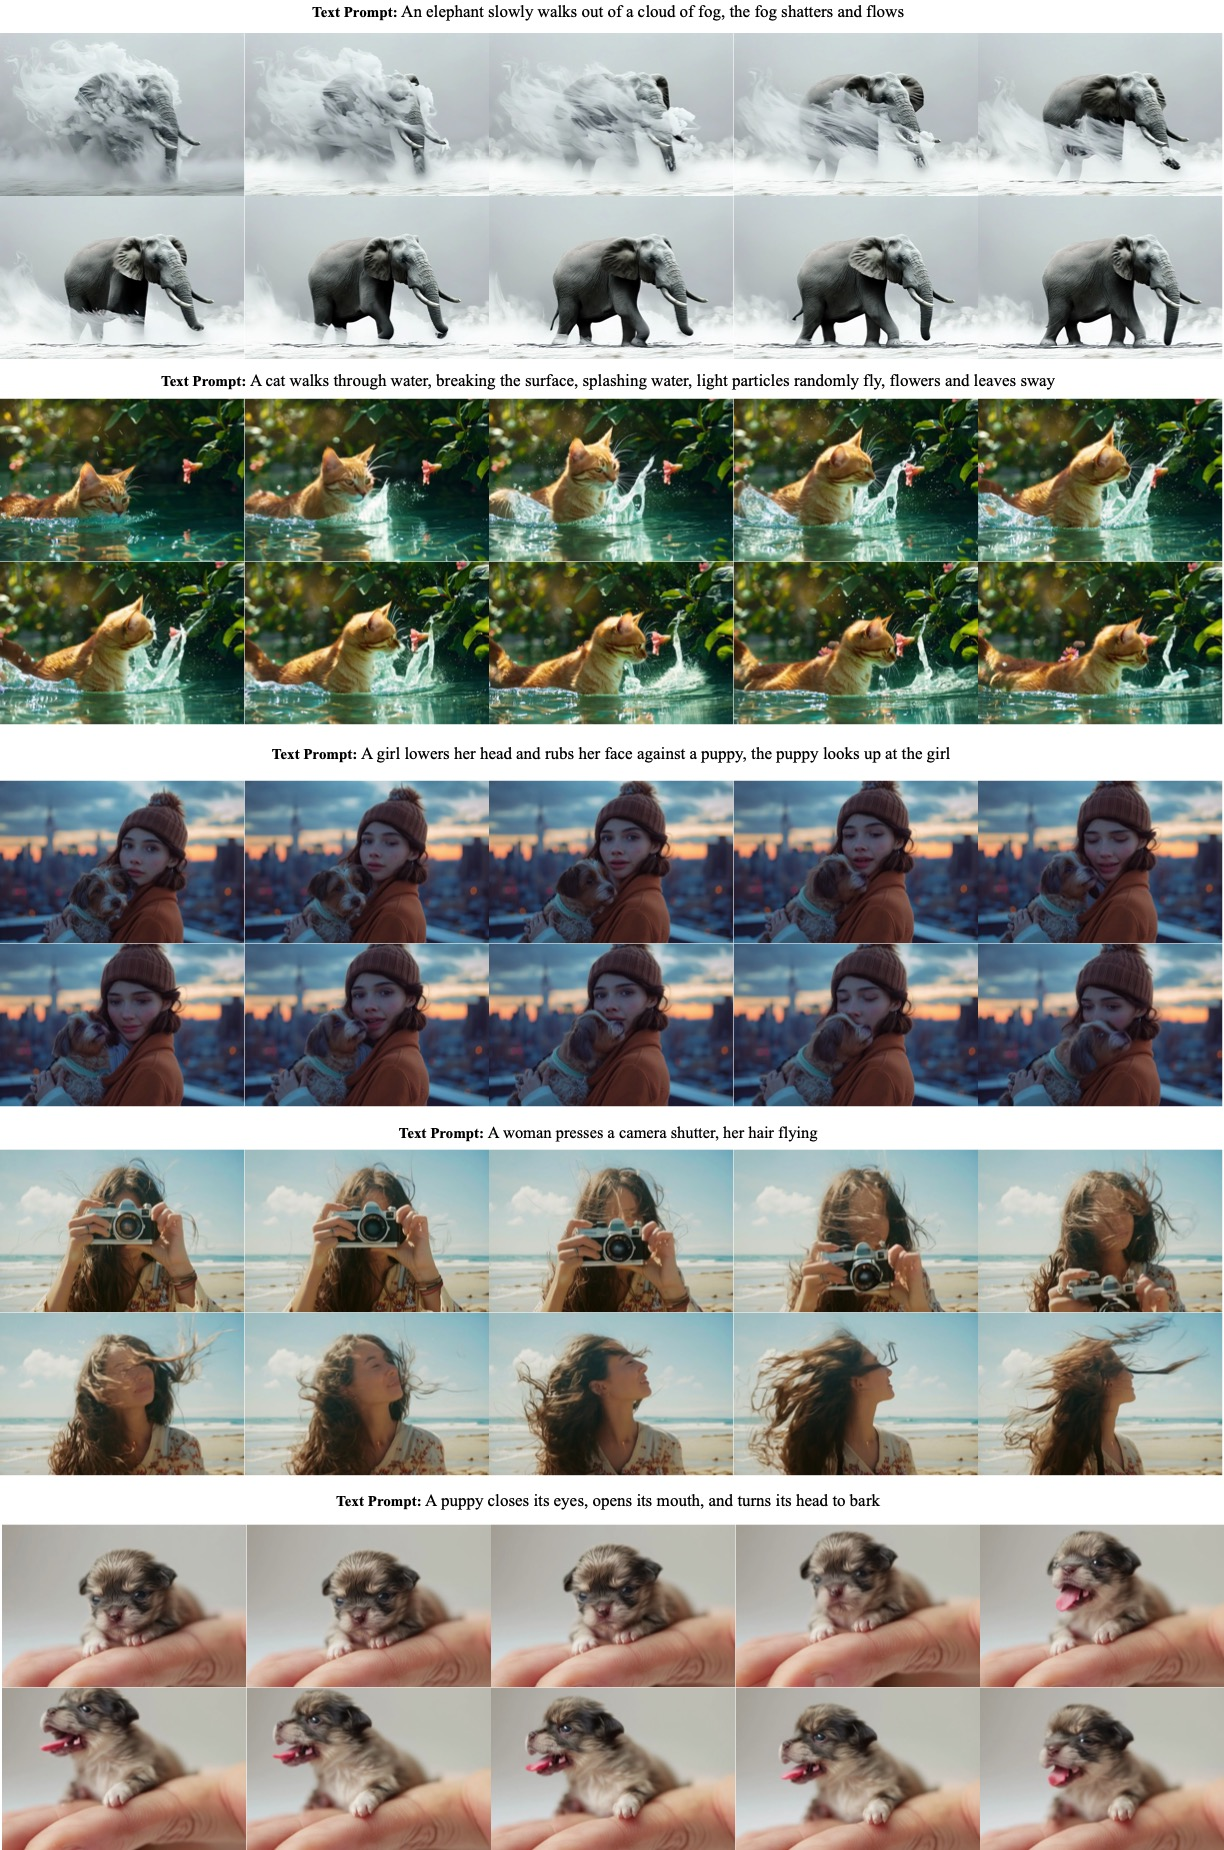
\includegraphics[width=\linewidth]{images/t2v/i2vgood2.jpg}
\end{center}
\caption{Image to video showcases.}
\label{fig:i2vgood2}
\end{figure}
\clearpage
\section{Caption Upsampler}
\label{ap:caption_upsampler}
To ensure that text input distribution during inference is as close as possible to the distribution during training, similar to \citep{betker2023improving}, we use a large language model to upsample the user's input during inference, making it more detailed and precise. Finetuned LLM can generate better prompts than zero/few-shot.

For image-to-video, we use the vision language model to upsample the prompt, such as GPT4V, CogVLM\citep{wang2023cogvlm}. 
\begin{promptbox}[Zero-shot prompt for Text Upsampler]
\noindent
\begin{verbatim}
You are part of a team of bots that create videos. You work 
with an assistant bot that will draw anything you say in 
square brackets. For example, outputting \" a beautiful 
morning in the woods with the sun peaking through the 
trees \" will trigger your partner bot to output a video
of a forest morning, as described. You will be prompted 
by people looking to create detailed, amazing videos. 
The way to accomplish this is to take their short prompts
and make them extremely detailed and descriptive.
There are a few rules to follow :
You will only ever output a single video description 
per user request.
When modifications are requested, you should not simply
make the description longer. You should refactor the
entire description to integrate the suggestions.

\end{verbatim}
\end{promptbox}


\section{Dense Video Caption Data Generation}
\label{ap:video_caption_gen}

In the pipeline for generating video captions, we extract one frame every two seconds for image captioning. Ultimately, we collected 50,000 data points to fine-tune the summary model. Below is the prompt we used for summarization with GPT-4:
\begin{promptbox}[Prompt for GPT-4 Summary]
\noindent
\begin{verbatim}
We extracted several frames from this video and described 
each frame using an image understanding model,  stored 
in the dictionary variable `image_captions: Dict[str: str]`.  
In `image_captions`,  the key is the second at which the image 
appears in the  video,  and the value is a detailed description 
of the image at that moment. Please describe the content of 
this video  in as much detail as possible,  based on the 
information  provided by `image_captions`,  including 
the objects, scenery, animals, characters, and camera 
movements within the video. \n image_captions={new_captions}\n 
You should output your summary directly,  and not mention
variables like `image_captions` in your response. 
Do not include `\\n' and the word 'video' in your response.  
Do not use introductory phrases such as: \"The video 
presents\", \"The video depicts\", \"This video showcases\", 
\"The video captures\" and so on.\n Please start the 
description with the video content directly, such as \"A man
first sits in a chair, then stands up and walks to the 
kitchen....\"\n Do not use phrases like: \"as the video 
progressed\" and \"Throughout the video\".\n Please describe 
the content of the video and the changes that occur, in 
chronological order.\n Please keep the description of this 
video within 100 English words.
\end{verbatim}
\end{promptbox}


\section{Video Caption Example}
\label{ap:video_caption_example}
Below we present some examples to compare the performance of the Panda-70M video captioning model and our CogVLM2-Caption model:


% \begin{figure}[h]
\begin{center}
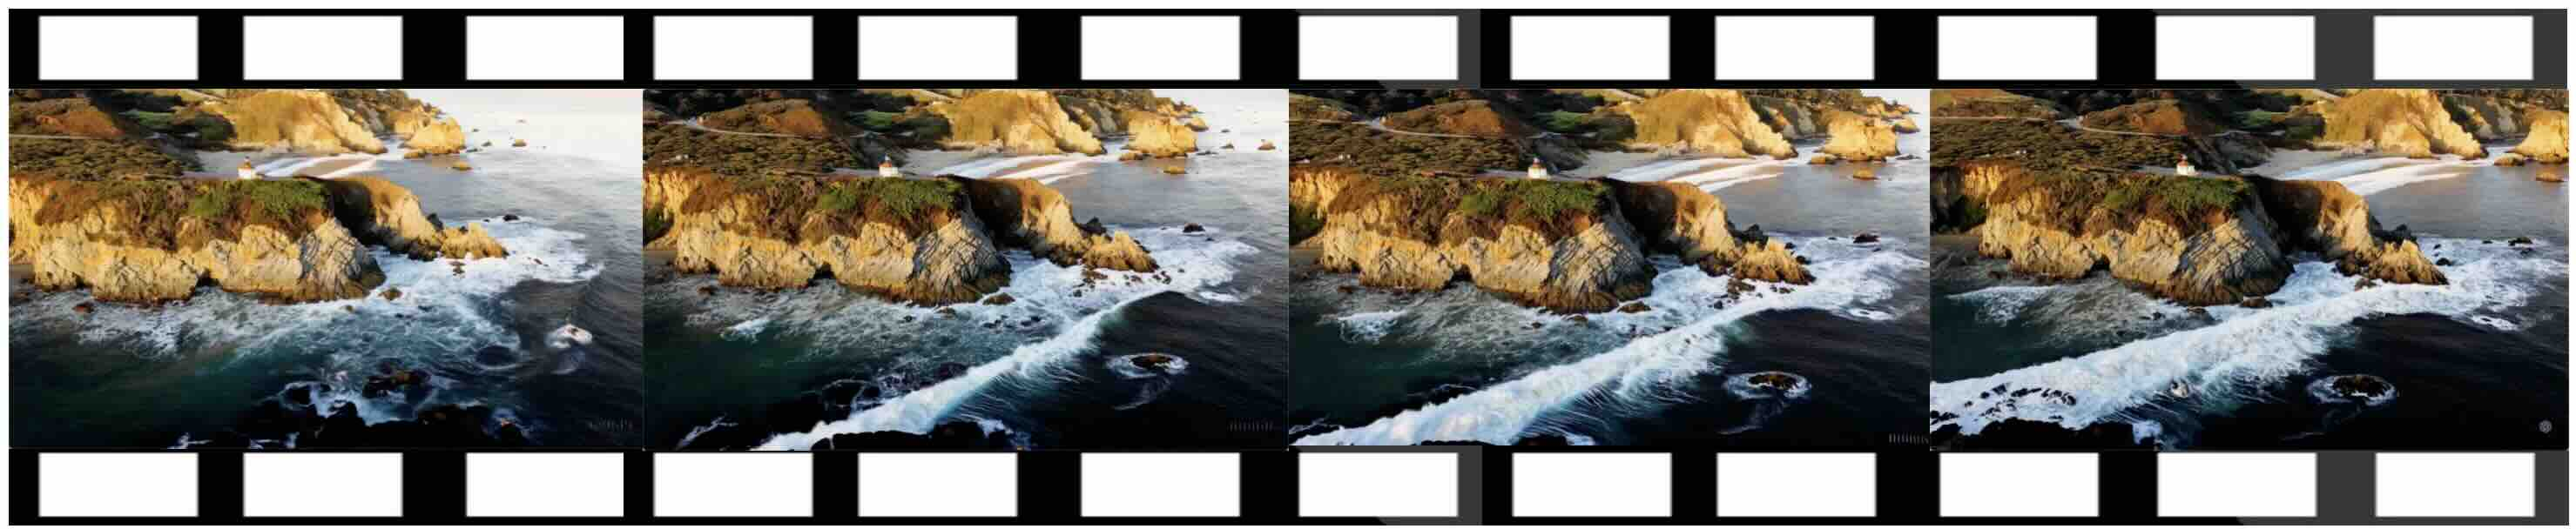
\includegraphics[width=0.9\linewidth]{images/caption_example1.jpg}
\end{center}
\end{figure}
% \begin{promptbox}[Caption Generated by Panda-70M]
% \begin{verbatim}
% There is an aerial view of a rocky coastline with waves 
% crashing against the shore, and a lighthouse on a cliff.
% \end{verbatim}
% \end{promptbox}
% \begin{promptbox}[Caption Generated by CogVLM2-Caption]
% \begin{verbatim}
% The video features a rugged coastline with cliffs descending 
% into the sea, where waves crash against rocks. A lighthouse 
% stands on a promontory, surrounded by greenery and bathed in
% sunlight that casts long shadows. The scene is tranquil yet 
% dynamic, with no human presence initially. As time passes, a 
% solitary house appears atop an elevated cliff, overlooking the 
% ocean. The landscape's colors transition from deep blues to 
% golden hues, suggesting dawn or dusk. Eventually, a road winds
% along the coast, leading to the secluded beach and lighthouse, 
% emphasizing the area's serene isolation amidst nature's 
% grandeur.
% \end{verbatim}
% \end{promptbox}


% \begin{figure}[h]
\begin{center}
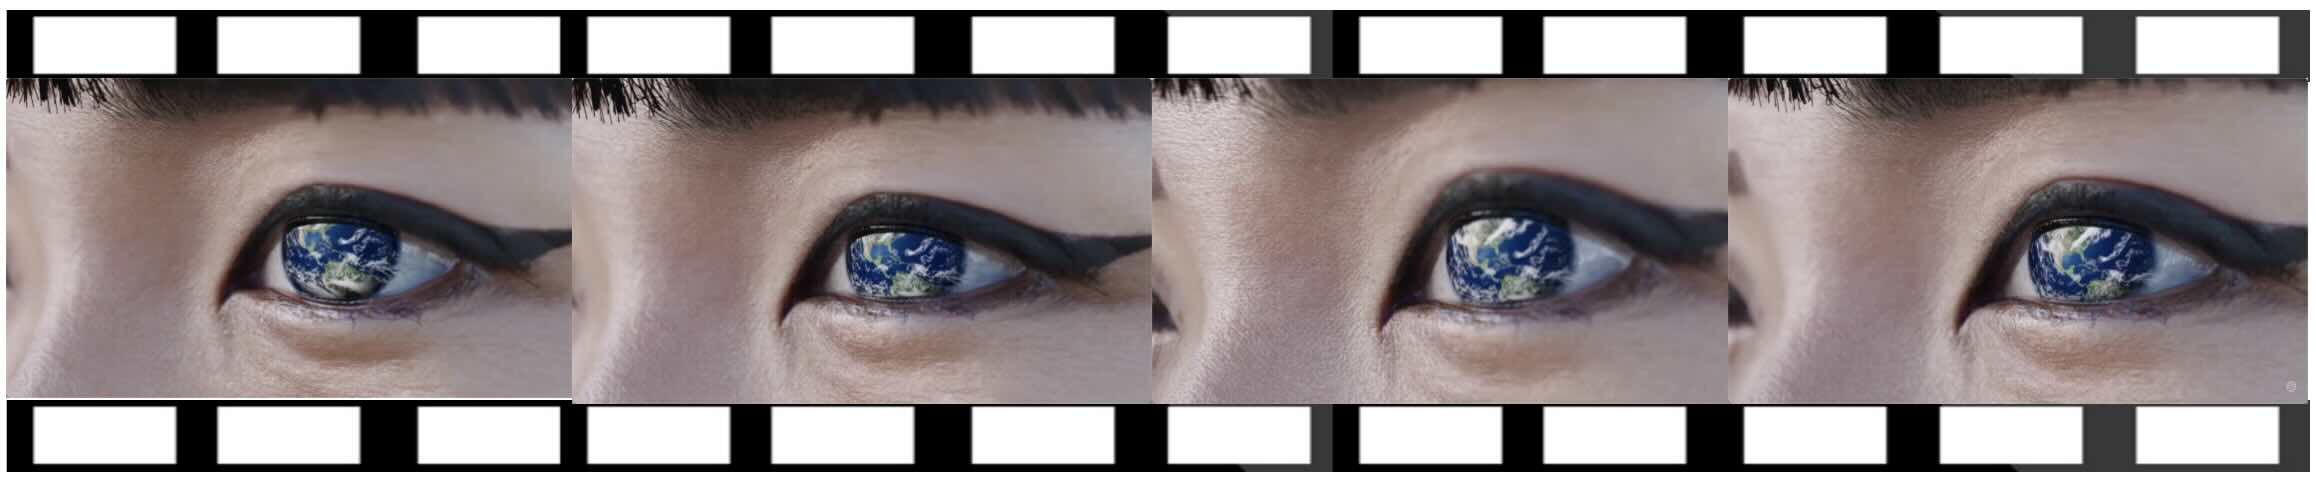
\includegraphics[width=0.9\linewidth]{images/caption_example2.jpg}
\end{center}
\end{figure}
% \begin{promptbox}[Caption Generated by Panda-70M]
% \begin{verbatim}
% A close up of a woman's eye with the earth in it.
% \end{verbatim}
% \end{promptbox}
% \begin{promptbox}[Caption Generated by CogVLM2-Caption]
% \begin{verbatim}
% A woman's eye, in sharp focus and detailed with a bold black
% eyeliner, reflects the Earth. The vivid colors of blue oceans
% and green continents stand out against her clear iris,
% symbolizing a deep connection between humanity and our planet.
% Her expression remains neutral throughout, emphasizing 
% introspection or awareness. As time passes, the reflection
% subtly shifts to include parts of Africa and Europe, suggesting
% a global perspective. The contrast between her dark eyelashes
% and light skin accentuates the visual metaphor for unity and 
% interconnectedness, while her gaze suggests contemplation on
% environmental issues or a profound sense of responsibility
% towards the world.
% \end{verbatim}
% \end{promptbox}


\begin{figure}[h]
\begin{center}
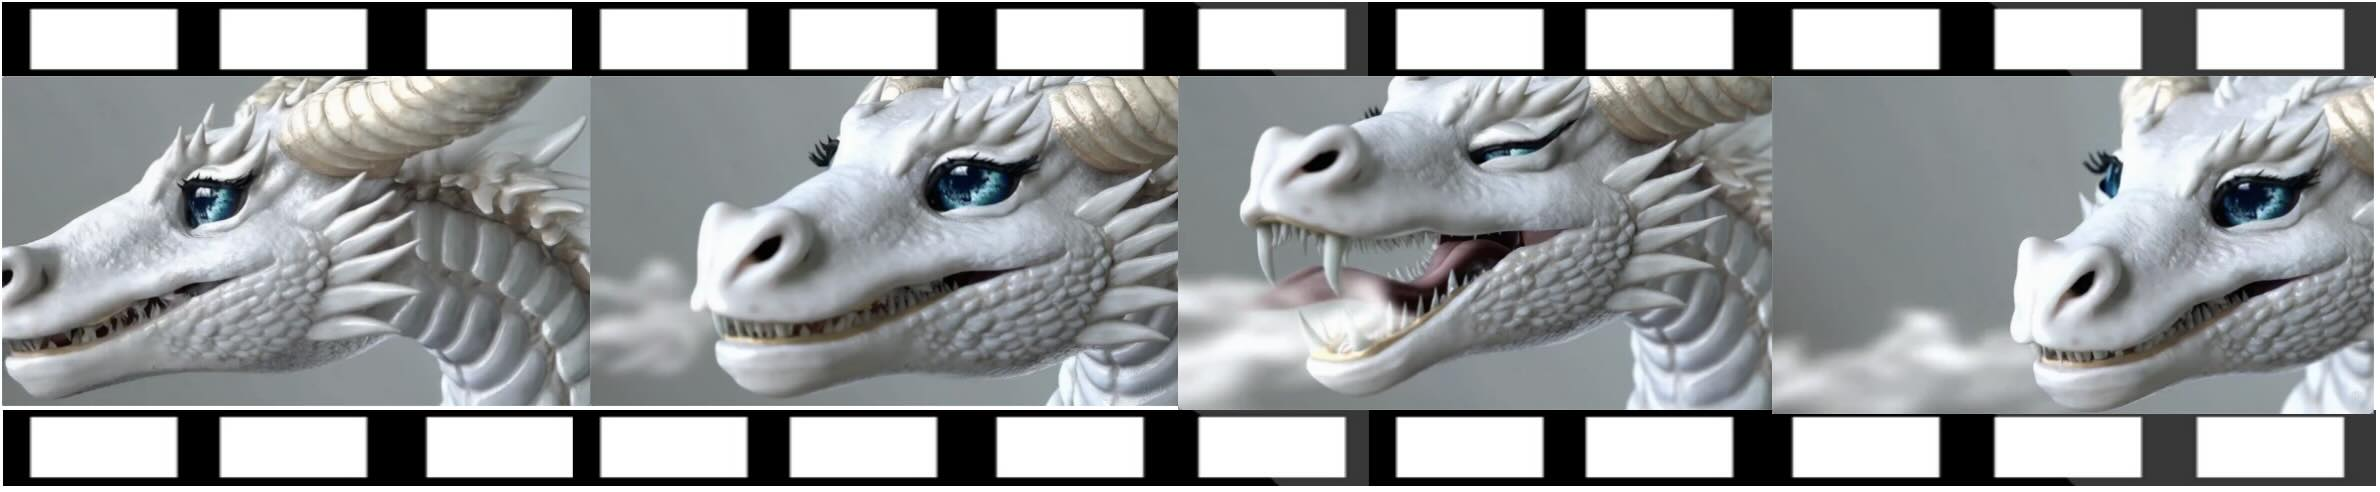
\includegraphics[width=0.9\linewidth]{images/caption_example3.jpg}
\end{center}
\end{figure}
\begin{promptbox}[Caption Generated by Panda-70M]
\begin{verbatim}
A close up of a white dragon with blue eyes.
\end{verbatim}
\end{promptbox}
\begin{promptbox}[Caption Generated by CogVLM2-Caption]
\begin{verbatim}
A meticulously crafted white dragon with a serene expression 
and piercing blue eyes is showcased in various close-ups, its 
scales detailed with golden highlights. Initially, the dragon's
horns are curved back, but as time passes, they change to 
spiraling gold, adding elegance. The creature's demeanor shifts 
from tranquil majesty to a more formidable presence, with its 
mouth agape revealing sharp teeth at times. Its expressions 
alternate between calmness and fierce determination, 
maintaining an air of mythical serenity throughout. The 
consistent neutral background focuses attention on the dragon's
textured features and expressive eyes.
\end{verbatim}
\end{promptbox}


\begin{figure}[h]
\begin{center}
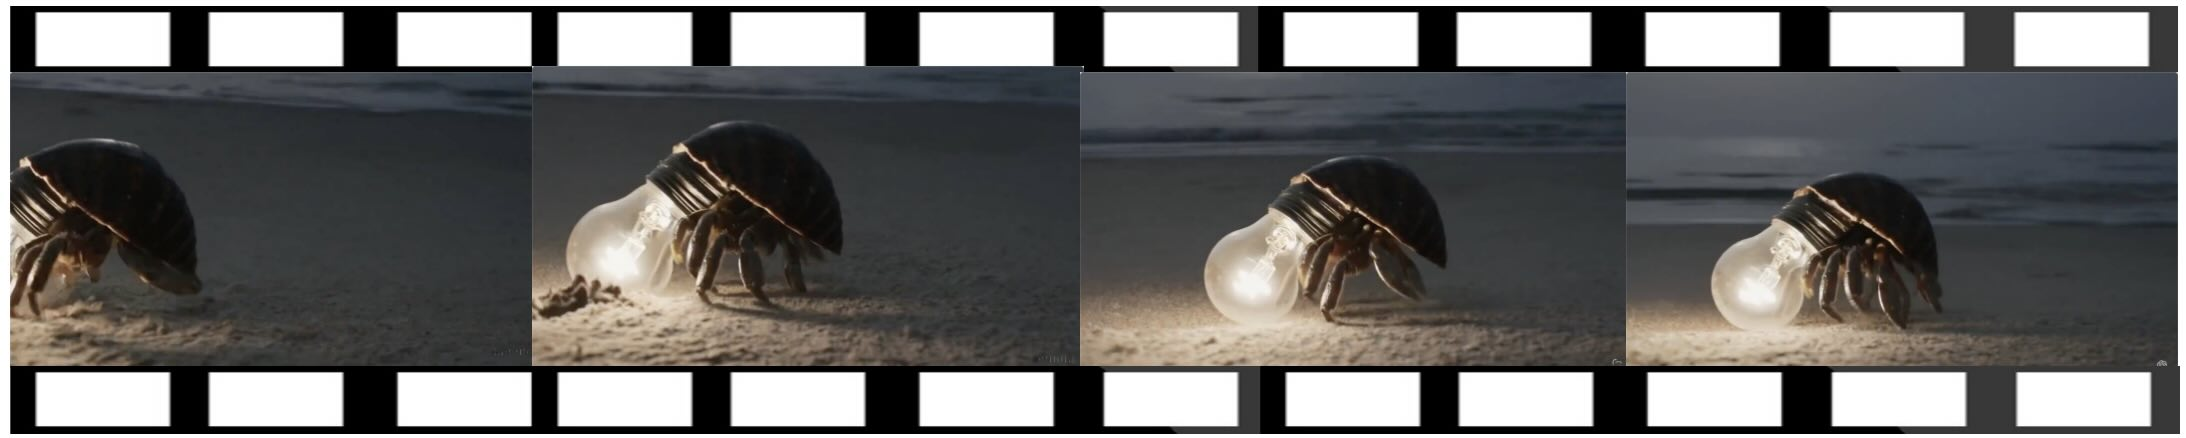
\includegraphics[width=0.9\linewidth]{images/caption_example4.jpg}
\end{center}
\end{figure}
\begin{promptbox}[Caption Generated by Panda-70M]
\begin{verbatim}
A crab is walking on the beach with a light bulb on its back.
\end{verbatim}
\end{promptbox}
\begin{promptbox}[Caption Generated by CogVLM2-Caption]
\begin{verbatim}
A hermit crab with a dark, glossy shell and reddish-brown legs
is seen carrying an illuminated light bulb on its back across 
the sandy terrain of a beach at night. The scene transitions 
from a soft glow to a more pronounced illumination as the crab
moves, highlighting its delicate limbs against the smooth sand
and tranquil sea backdrop. This surreal tableau blends natural
beauty with human ingenuity, creating a serene yet whimsical 
atmosphere that emphasizes the crab's unique adaptation and the
contrast between nature and technology in this quiet nocturnal
setting.
\end{verbatim}
\end{promptbox}


\begin{figure}[h]
\begin{center}
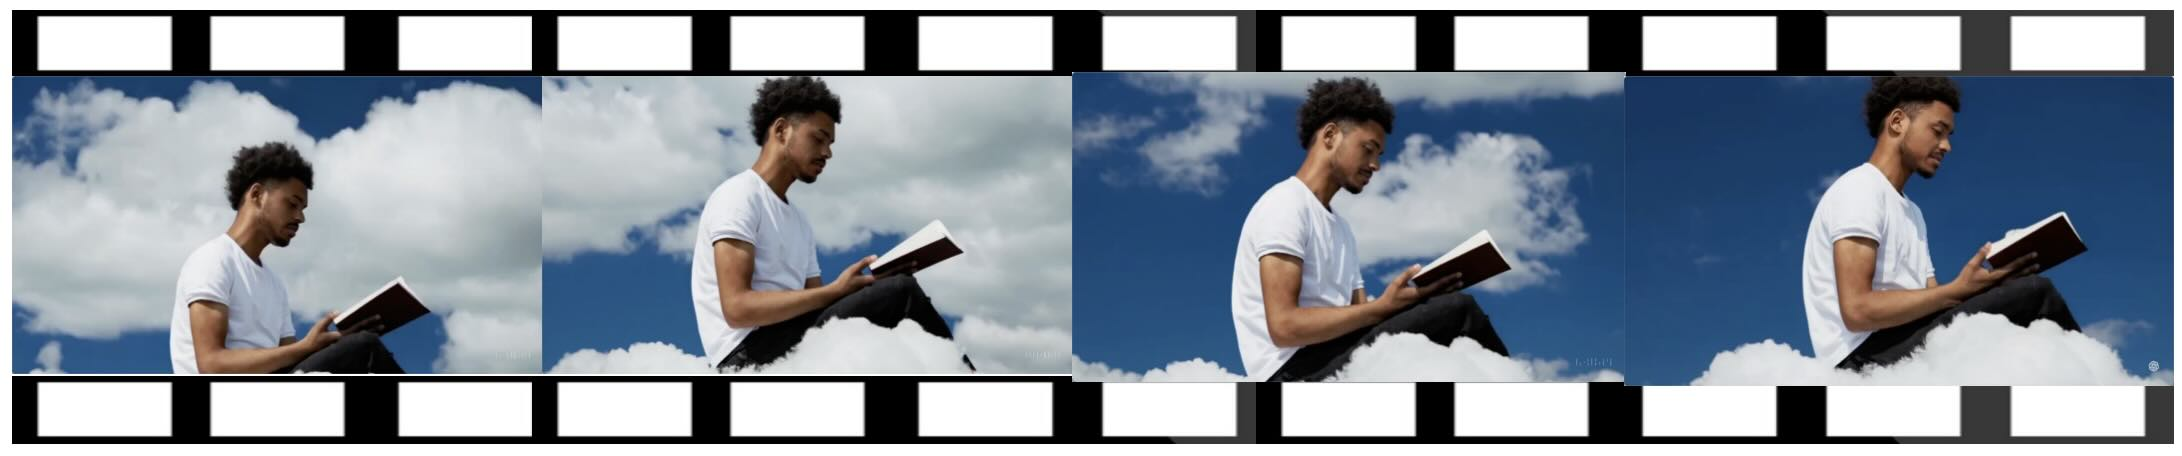
\includegraphics[width=0.9\linewidth]{images/caption_example5.jpg}
\end{center}
\end{figure}
\begin{promptbox}[Caption Generated by Panda-70M]
\begin{verbatim}
A young black man is sitting on a cloud and reading a book 
with a blue sky in the background.
\end{verbatim}
\end{promptbox}
\begin{promptbox}[Caption Generated by CogVLM2-Caption]
\begin{verbatim}
A young Black man with an afro hairstyle and a neatly trimmed 
beard is seen sitting cross-legged on fluffy white clouds, 
deeply engrossed in reading a book with a red cover. He wears 
a plain white T-shirt and dark pants against a vivid blue sky 
dotted with cumulus clouds. Throughout the scenes, his 
expression remains one of deep concentration and peaceful 
contemplation, highlighting a moment of intellectual pursuit 
amidst nature's grandeur. The imagery suggests a serene 
atmosphere that emphasizes solitude and introspection, with no 
other people or objects around him.
\end{verbatim}
\end{promptbox}


% \begin{figure}[h]
\begin{center}
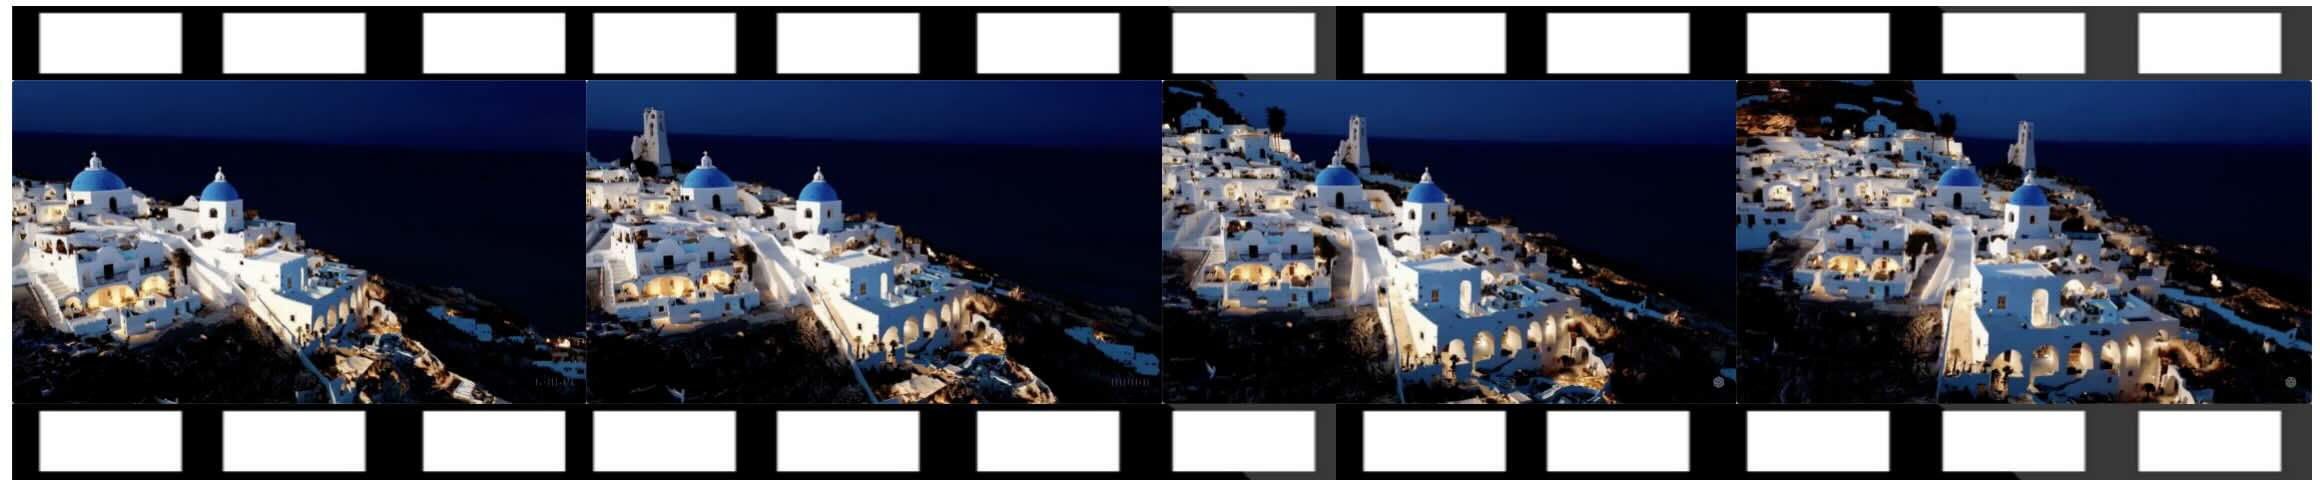
\includegraphics[width=0.9\linewidth]{images/caption_example6.jpg}
\end{center}
\end{figure}
% \begin{promptbox}[Caption Generated by Panda-70M]
% \begin{verbatim}
% A white church on a cliff overlooking the ocean at night.
% \end{verbatim}
% \end{promptbox}
% \begin{promptbox}[Caption Generated by CogVLM2-Caption]
% \begin{verbatim}
% A picturesque evening descends on a cliffside village, 
% showcasing whitewashed buildings with blue domes that glow 
% against the darkening sky. The Aegean Sea mirrors this 
% celestial hue, creating a serene tableau devoid of people and 
% vehicles. As time passes, the scene remains tranquil, 
% illuminated by golden lights from within homes and lit 
% pathways weaving between structures. A solitary windmill 
% stands out, symbolizing local culture amidst the peaceful 
% setting. The absence of visible human activity emphasizes the 
% stillness and beauty of the coastal hamlet, inviting 
% contemplation in its embrace.
% \end{verbatim}
% \end{promptbox}


% \begin{figure}[h]
\begin{center}
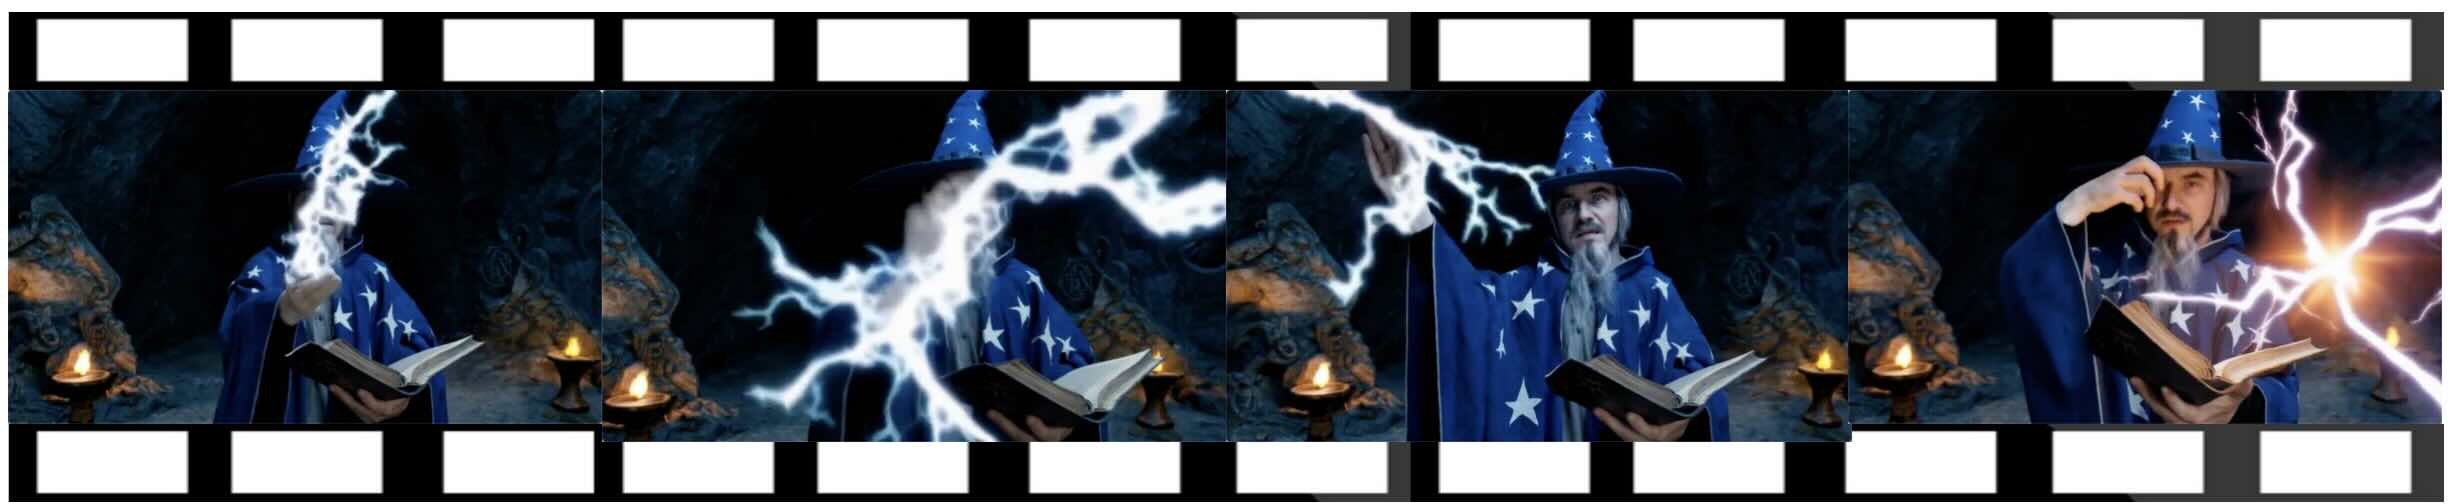
\includegraphics[width=0.9\linewidth]{images/caption_example7.jpg}
\end{center}
\end{figure}
% \begin{promptbox}[Caption Generated by Panda-70M]
% \begin{verbatim}
% A man dressed as a wizard is holding a book and a lightning
% bolt is coming out of it.
% \end{verbatim}
% \end{promptbox}
% \begin{promptbox}[Caption Generated by CogVLM2-Caption]
% \begin{verbatim}
% A man dressed as a wizard, with a blue robe adorned with white
% stars and a matching pointed hat, stands in a dark cave. He is 
% engaged in casting spells from an open book, surrounded by 
% mystical flames that illuminate the scene. Throughout the 
% sequence, his right hand is raised to channel bright lightning
% bolts towards unseen targets, while his left hand holds the
% book firmly. His expression remains focused and serious, 
% suggesting deep concentration on his magical endeavors. The 
% atmosphere of mystery and ancient magic is enhanced by the 
% surrounding darkness and the vivid display of light and shadow.
% \end{verbatim}
% \end{promptbox}
\clearpage
\section{Video to Video via CogVideoX and CogVLM2-Caption}
\label{ap:v2v}

In this section, we present several examples of video-to-video generation using CogVideoX and CogVLM2-Caption. Specifically, we first input the original video into CogVLM2-Caption to obtain the video's caption, and then feed this caption into the CogVideoX model to generate a new video. From the examples below, it can be seen that our pipeline achieves a high degree of fidelity to the original video:

\begin{figure}[h]
\begin{center}
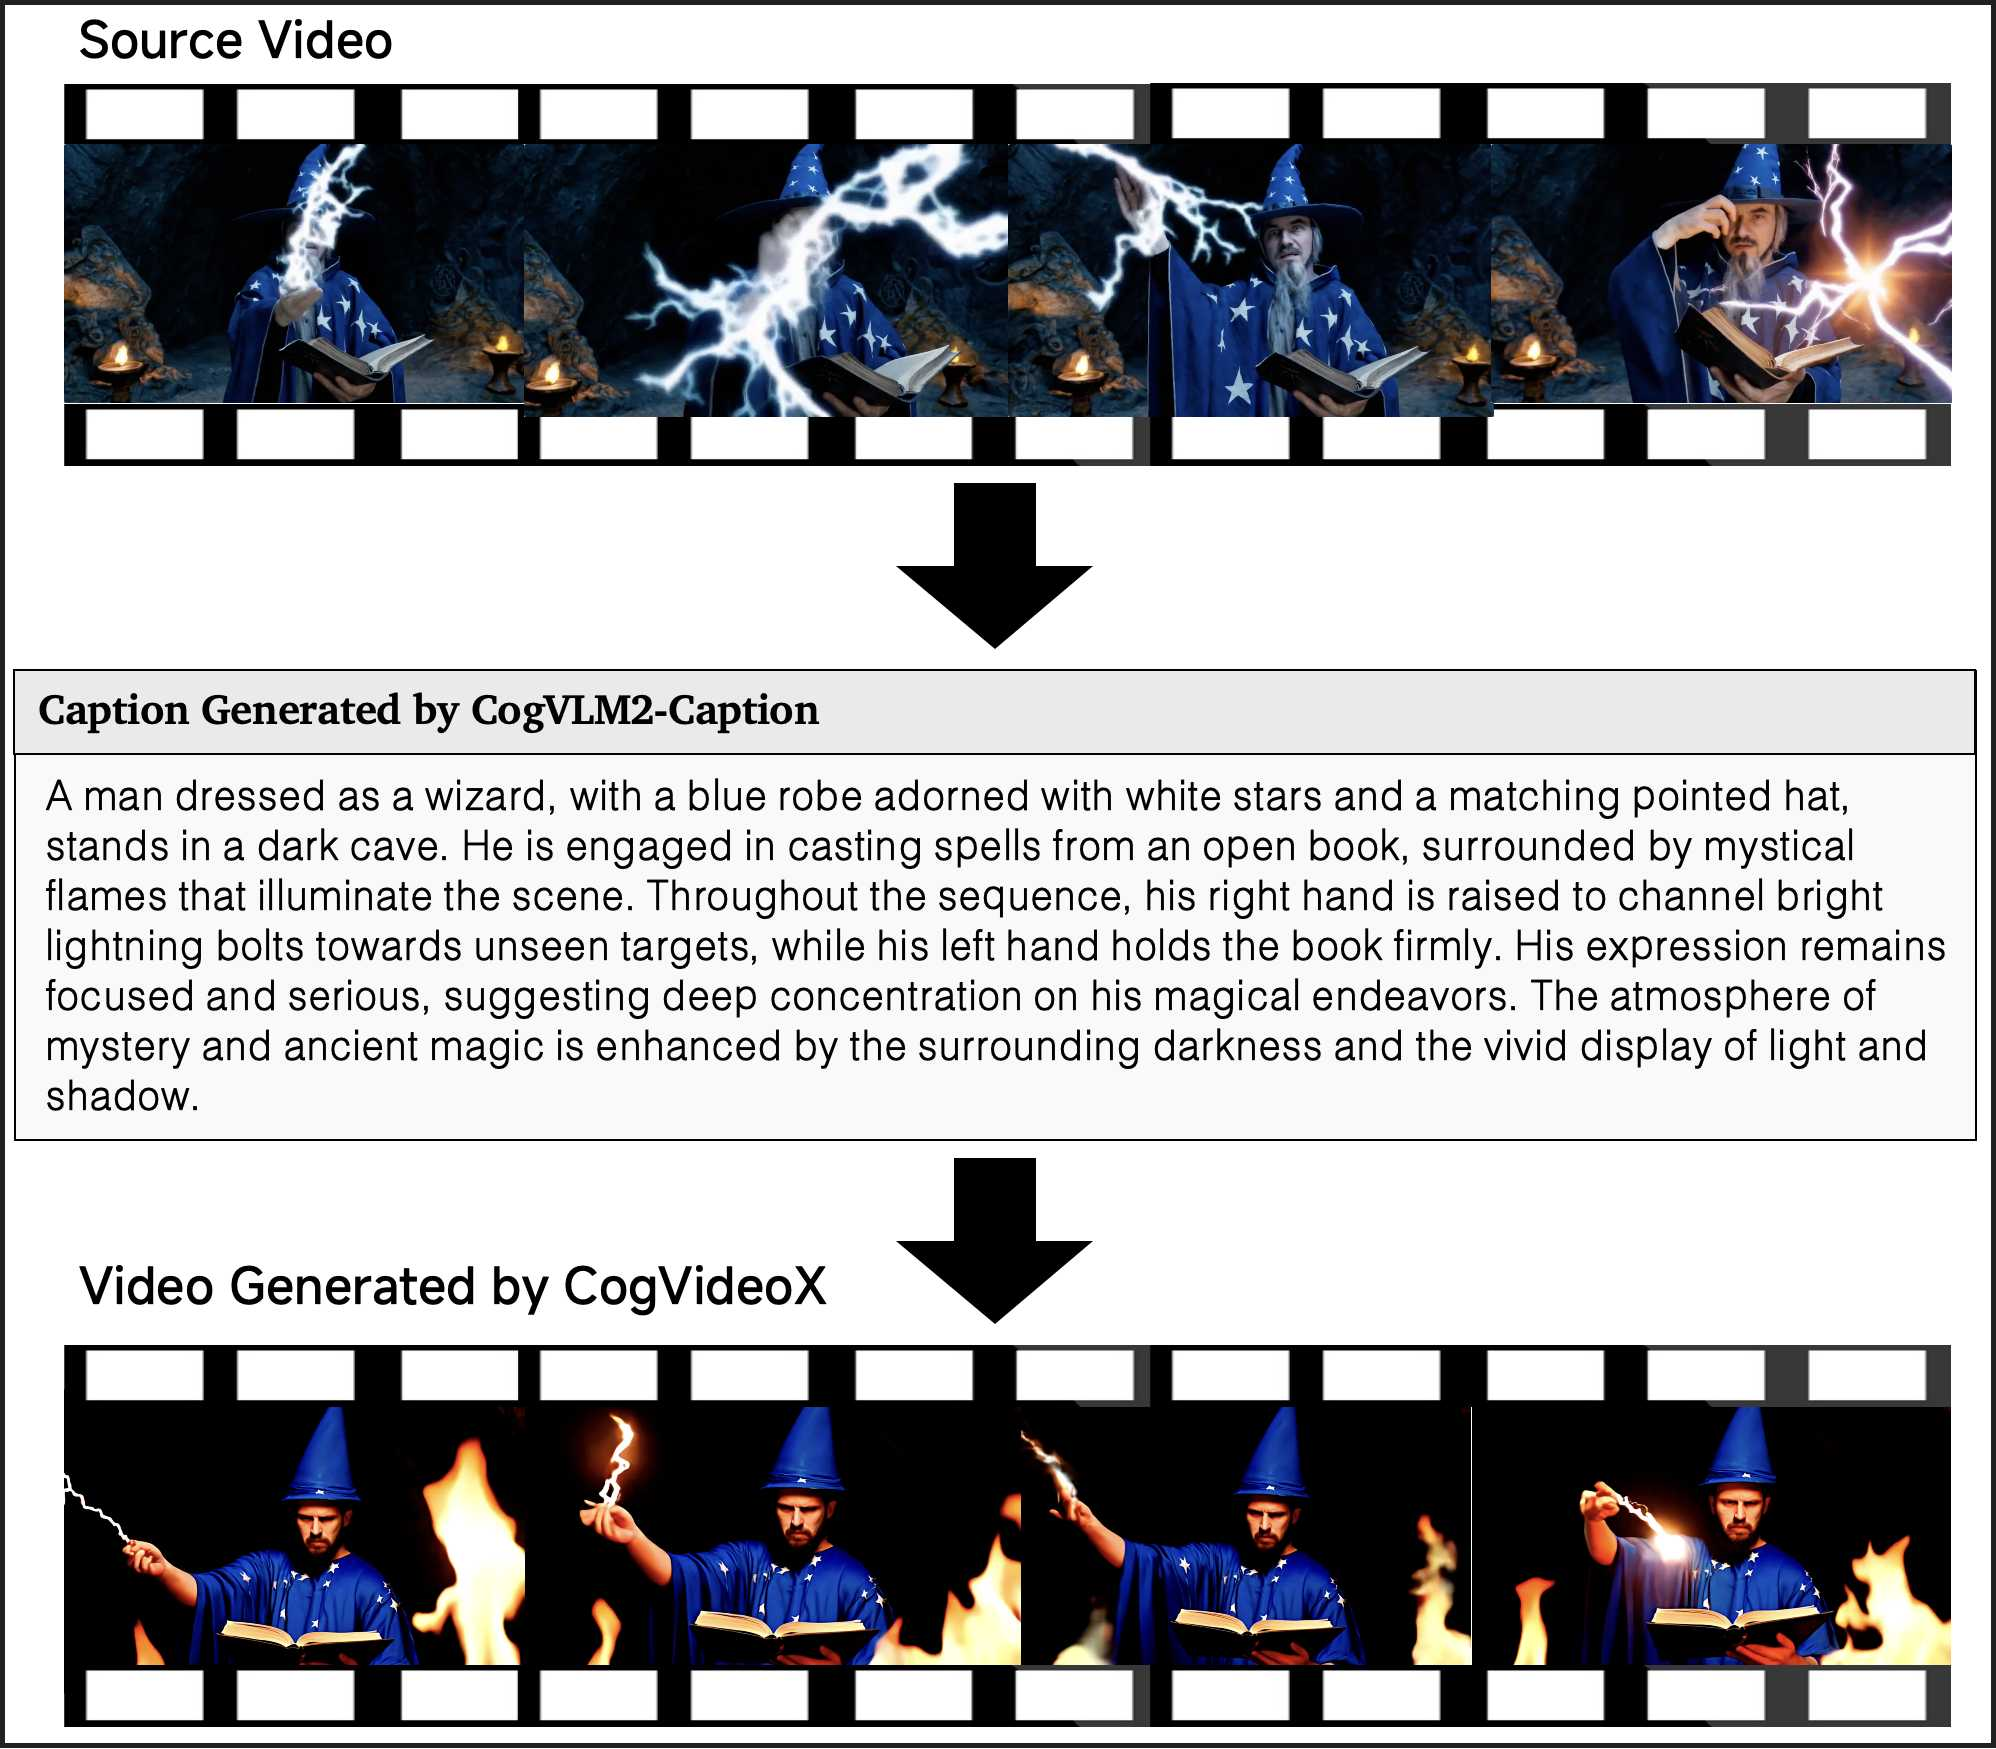
\includegraphics[width=0.9\linewidth]{images/v2v/v2v_1.jpg}
\end{center}
\end{figure}

\begin{figure}[h]
\begin{center}
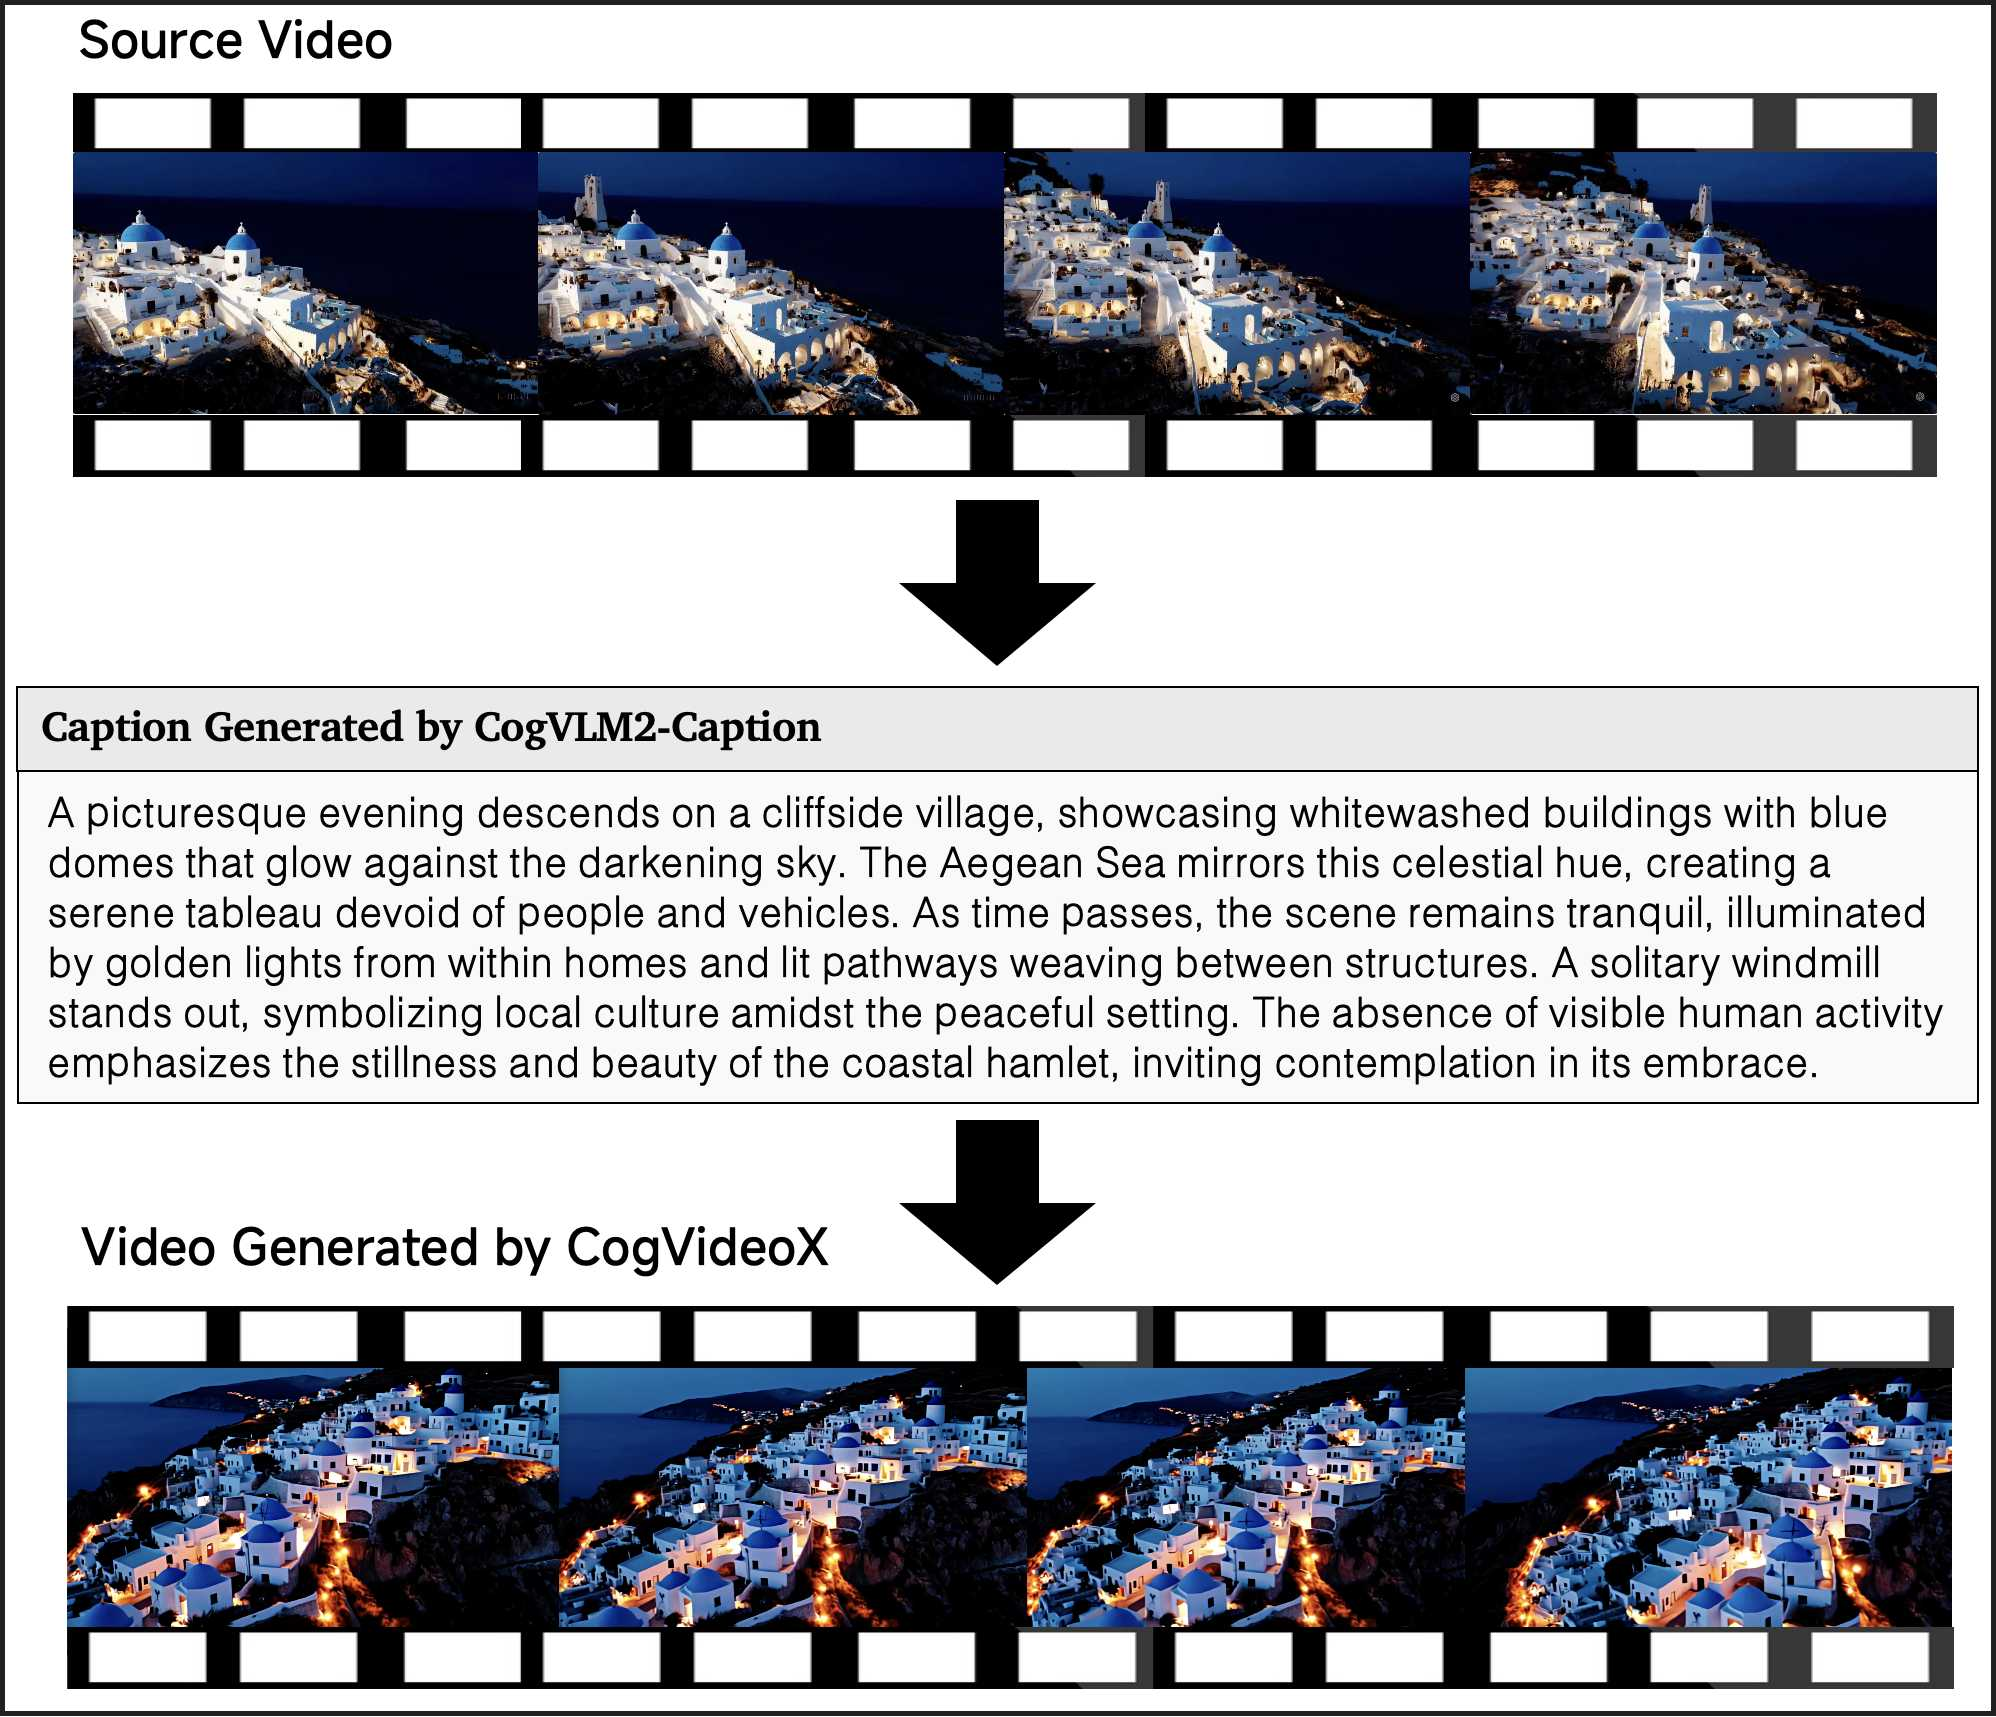
\includegraphics[width=0.9\linewidth]{images/v2v/v2v_2.jpg}
\end{center}
\end{figure}

\begin{figure}[h]
\begin{center}
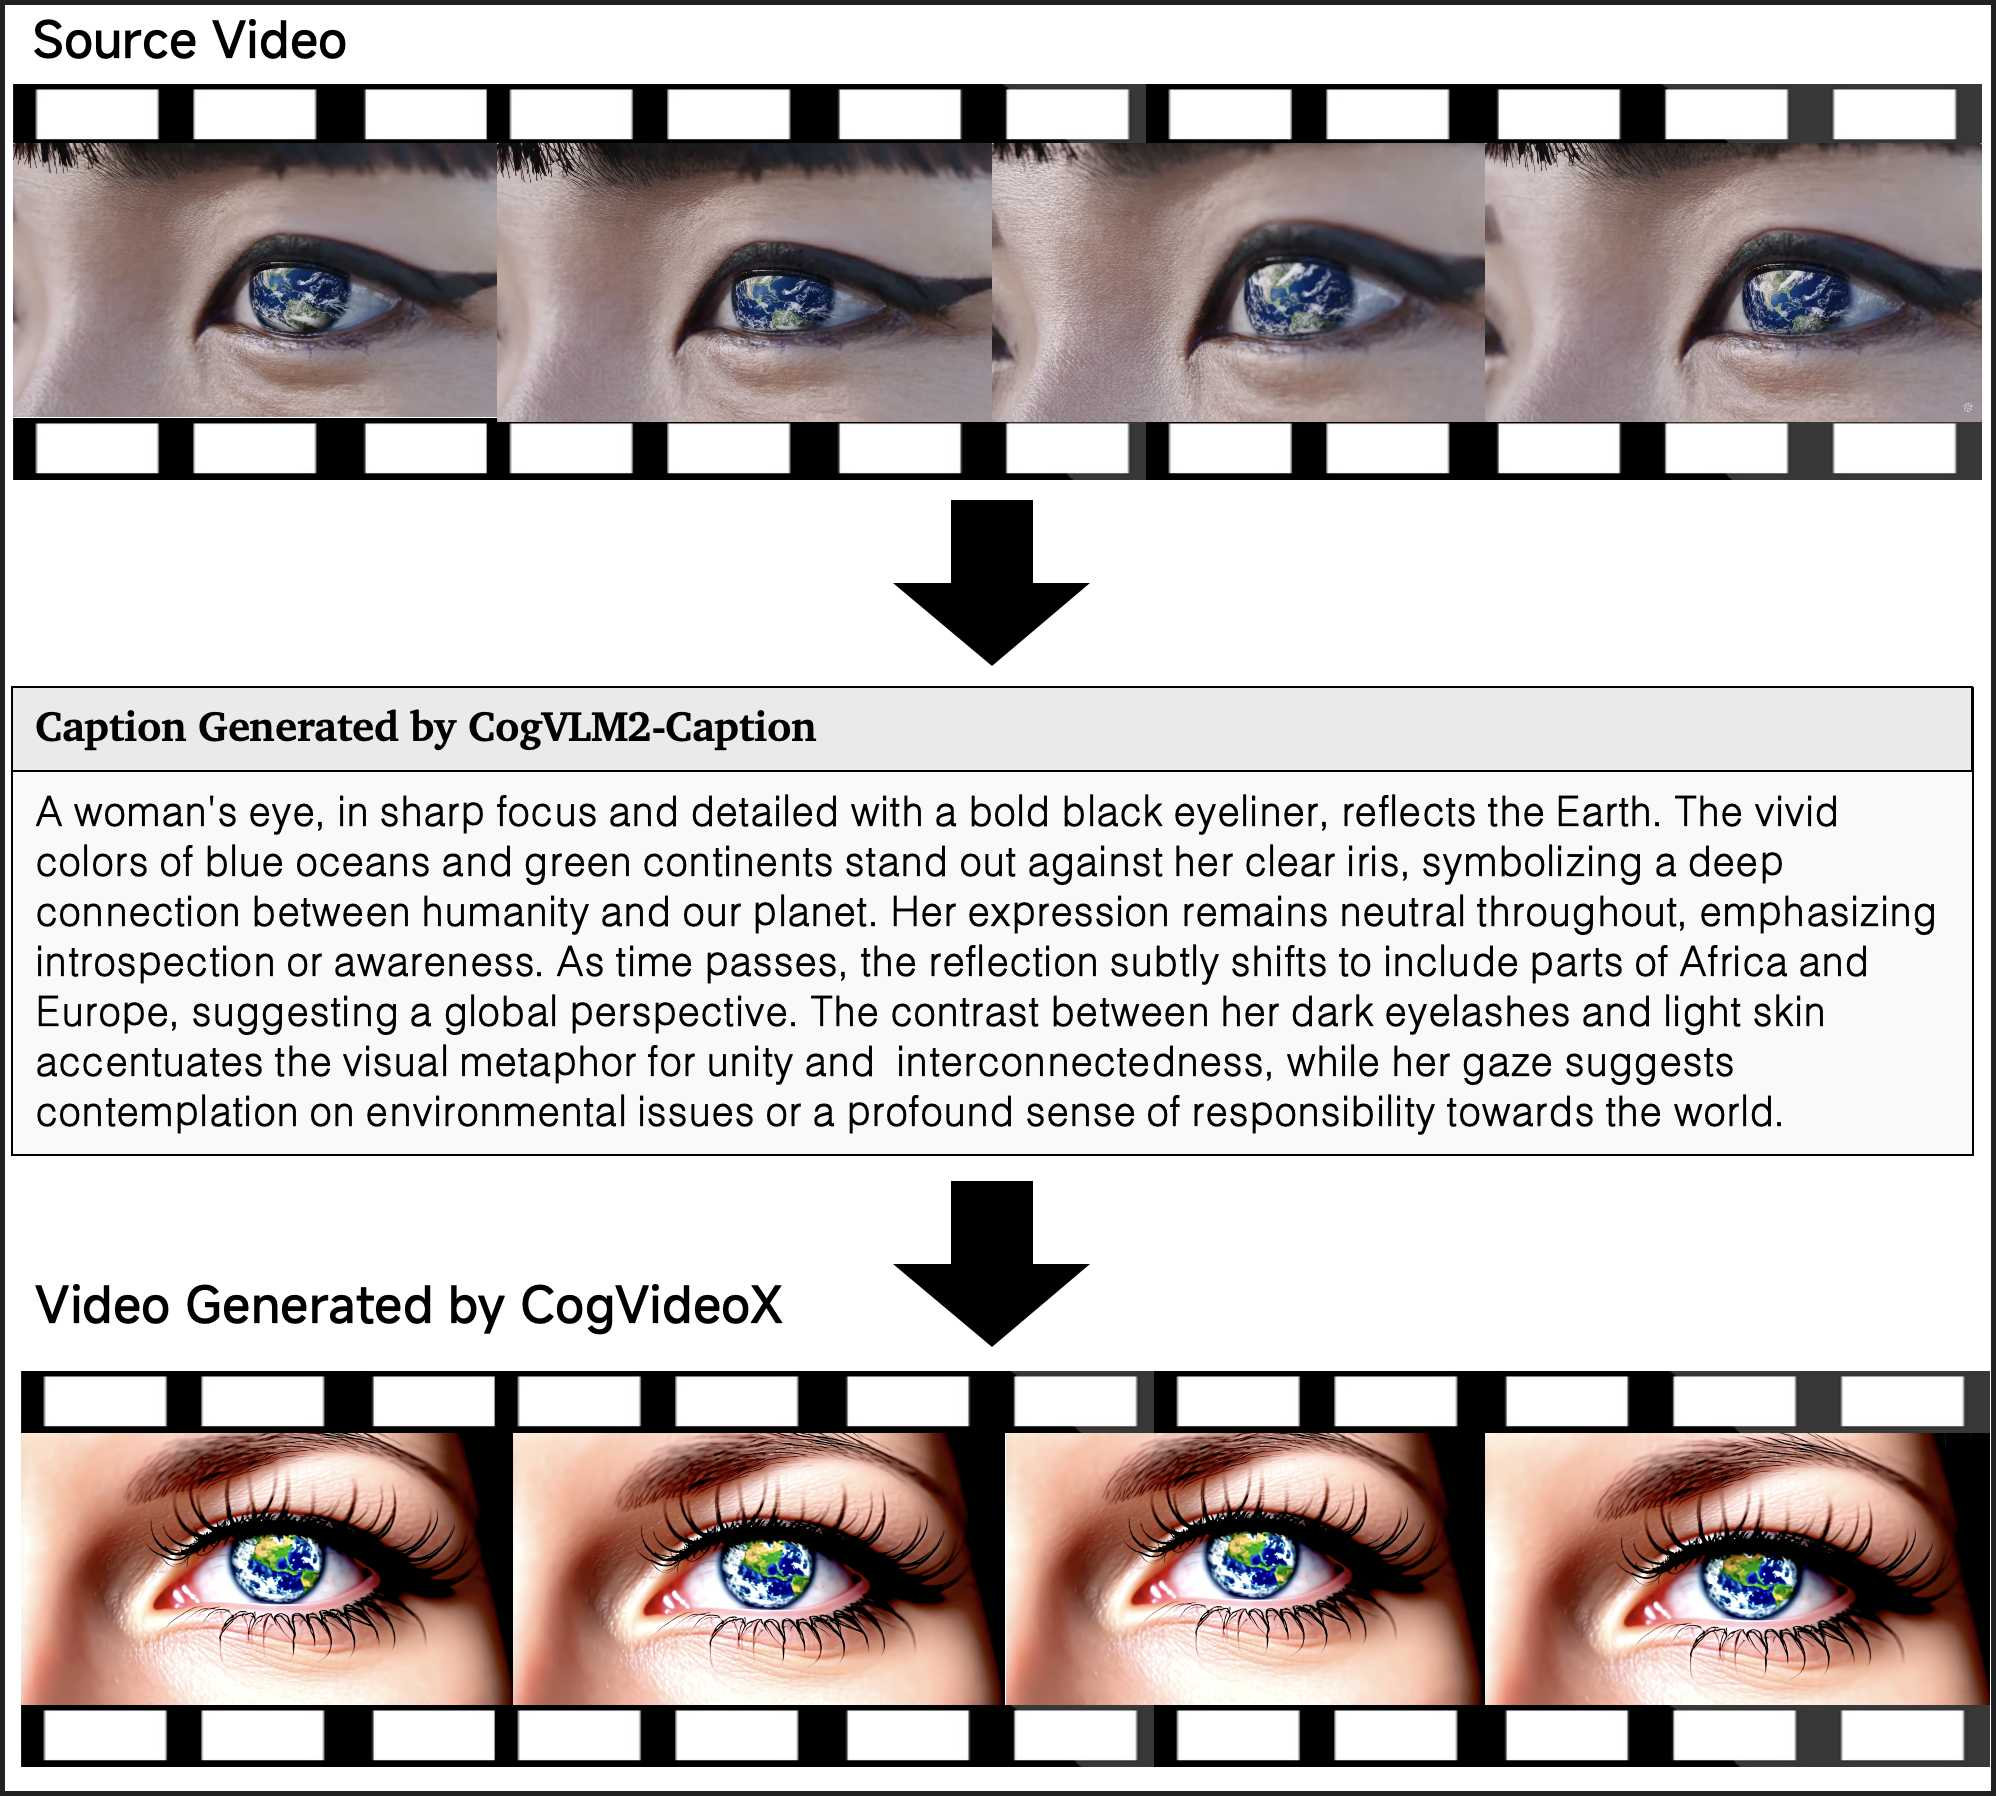
\includegraphics[width=0.9\linewidth]{images/v2v/v2v_3.jpg}
\end{center}
\end{figure}


\begin{table}[!ht]
\centering
\label{sample-table}
\small
\vspace{-5pt}
\caption{Human evaluation between CogVideoX and Kling.}
\label{table:human_eva}
\resizebox{0.75\linewidth}{!}{
    \begin{tabular}{cccccc}
    \toprule
        Model & \Centerstack{Sensory\\Quality} & \Centerstack{Instruction\\Following}&\Centerstack{Physics\\Simulation} & \Centerstack{Cover\\Quality} & 
        \Centerstack{Total\\Score} \\ 
        \midrule
        Kling & 0.638 & 0.367 & 0.561 & 0.668 & 2.17 \\
        \midrule
         {\bf CogVideoX-5B} & {\bf 0.722} & {\bf 0.495} & {\bf 0.667} & {\bf 0.712} & {\bf 2.74}  \\
        \bottomrule
    \end{tabular}
}
\end{table}

\end{document}